%%%%%%%%%%%%%%%%%%%%%%%%%%%%%%%%%%%%%%%%%%%%%%%%%%%%%%%%%%%%%%%%%%%%%%%%%%%%%
%%%
%%% File: utthesis2.doc, version 2.0jab, February 2002
%%%
%%% Based on: utthesis.doc, version 2.0, January 1995
%%% =============================================
%%% Copyright (c) 1995 by Dinesh Das.  All rights reserved.
%%% This file is free and can be modified or distributed as long as
%%% you meet the following conditions:
%%%
%%% (1) This copyright notice is kept intact on all modified copies.
%%% (2) If you modify this file, you MUST NOT use the original file name.
%%%
%%% This file contains a template that can be used with the package
%%% utthesis.sty and LaTeX2e to produce a thesis that meets the requirements
%%% of the Graduate School of The University of Texas at Austin.
%%%
%%% All of the commands defined by utthesis.sty have default values (see
%%% the file utthesis.sty for these values).  Thus, theoretically, you
%%% don't need to define values for any of them; you can run this file
%%% through LaTeX2e and produce an acceptable thesis, without any text.
%%% However, you probably want to set at least some of the macros (like
%%% \thesisauthor).  In that case, replace "..." with appropriate values,
%%% and uncomment the line (by removing the leading %'s).
%%%
%%%%%%%%%%%%%%%%%%%%%%%%%%%%%%%%%%%%%%%%%%%%%%%%%%%%%%%%%%%%%%%%%%%%%%%%%%%%%

\documentclass[a4paper, 12pt, oneside]{report}         %% LaTeX2e document.
\usepackage {tcdthesis}              %% Preamble.

%%For loading graphic files
\usepackage{graphicx}
%% subfigure
\usepackage{caption}
\usepackage{subcaption}
%% bookmark
\usepackage{hyperref}
%% url
\usepackage{url}
\usepackage{textgreek}
%% image path
\graphicspath{{../img/CGVC2015/}{../img/EuroVis2015/}{../img/TransferReport/}{../img/EurasiaGraphics2014/images/}{../img/EurasiaGraphics2014/images1/}{../img/EurasiaGraphics2014/images2/}{../img/EurasiaGraphics2014/images3/}{../img/EurasiaGraphics2014/images4/}}
\usepackage{lmodern} %Type1-font for non-english texts and characters

%% Math Packages %%%%%%%%%%%%%%%%%%%%%%%%%%%%%%%%%%%%%%%%%%%%
\usepackage{amsmath}
\usepackage{amsthm}
\usepackage{amsfonts}

% other packages
\usepackage{cite}
\usepackage{braket}
\newcommand\addtag{\refstepcounter{equation}\tag{\theequation}}

% \mastersthesis                     %% Uncomment one of these; if you don't
\phdthesis                         %% use either, the default is \phdthesis.

%\thesisdraft                       %% Uncomment this if you want a draft
                                     %% version; this will print a timestamp
                                     %% on each page of your thesis.

\leftchapter                       %% Uncomment one of these if you want
%\centerchapter                      %% left-justified, centered or
% \rightchapter                      %% right-justified chapter headings.
                                     %% Chapter headings includes the
                                     %% Contents, Acknowledgments, Lists
                                     %% of Tables and Figures and the Vita.
                                     %% The default is \centerchapter.

% \singlespace                       %% Uncomment one of these if you want
\oneandhalfspace                   %% single-spacing, space-and-a-half
% \doublespace                       %% or double-spacing; the default is
                                     %% \oneandhalfspace, which is the
                                     %% minimum spacing accepted by the
                                     %% Graduate School.

\renewcommand{\thesisauthor}{Shengzhou Luo}            %% Your official UT name.
\renewcommand{\thesismonth}{August}                  %% Your month of graduation.
\renewcommand{\thesisyear}{2015}                      %% Your year of graduation.
\renewcommand{\thesistitle}{Information-Guided Transfer Function Optimization and Enhancements for Volume Visualization}            %% The title of your thesis; use mixed-case.
\renewcommand{\thesisauthorpreviousdegrees}{MSc}  %% Your previous degrees, abbreviated; separate multiple degrees by commas.
\renewcommand{\thesissupervisor}{John Dingliana}      %% Your thesis supervisor; use mixed-case and don't use any titles or degrees.
% \renewcommand{\thesiscosupervisor}{}                %% Your PhD. thesis co-supervisor; if any.

% \renewcommand{\thesiscommitteemembera}{}
% \renewcommand{\thesiscommitteememberb}{}
% \renewcommand{\thesiscommitteememberc}{}
% \renewcommand{\thesiscommitteememberd}{}
% \renewcommand{\thesiscommitteemembere}{}
% \renewcommand{\thesiscommitteememberf}{}
% \renewcommand{\thesiscommitteememberg}{}
% \renewcommand{\thesiscommitteememberh}{}
% \renewcommand{\thesiscommitteememberi}{}

\renewcommand{\thesisauthoraddress}{Dublin, Ireland}

\renewcommand{\thesisdedication}{}     %% Your dedication, if you have one; use "\\" for sbreaks.


%%%%%%%%%%%%%%%%%%%%%%%%%%%%%%%%%%%%%%%%%%%%%%%%%%%%%%%%%%%%%%%%%%%%%%%%%%%%%
%%%
%%% The following commands are all optional, but useful if your requirements
%%% are different from the default values in utthesis.sty.  To use them,
%%% simply uncomment (remove the leading %) the line(s).

% \renewcommand{\thesiscommitteesize}{...}
                                     %% Uncomment this only if your thesis
                                     %% committee does NOT have 5 members
                                     %% for \phdthesis or 2 for \mastersthesis.
                                     %% Replace the "..." with the correct
                                     %% number of members.

% \renewcommand{\thesisdegree}{...}  %% Uncomment this only if your thesis
                                     %% degree is NOT "DOCTOR OF PHILOSOPHY"
                                     %% for \phdthesis or "MASTER OF ARTS"
                                     %% for \mastersthesis.  Provide the
                                     %% correct FULL OFFICIAL name of
                                     %% the degree.

% \renewcommand{\thesisdegreeabbreviation}{...}
                                     %% Use this if you also use the above
                                     %% command; provide the OFFICIAL
                                     %% abbreviation of your thesis degree.

% \renewcommand{\thesistype}{...}    %% Use this ONLY if your thesis type
                                     %% is NOT "Dissertation" for \phdthesis
                                     %% or "Thesis" for \mastersthesis.
                                     %% Provide the OFFICIAL type of the
                                     %% thesis; use mixed-case.

% \renewcommand{\thesistypist}{...}  %% Use this to specify the name of
                                     %% the thesis typist if it is anything
                                     %% other than "the author".

%%%
%%%%%%%%%%%%%%%%%%%%%%%%%%%%%%%%%%%%%%%%%%%%%%%%%%%%%%%%%%%%%%%%%%%%%%%%%%%%%



\begin{document}                                  %% BEGIN THE DOCUMENT

%\thesistitlepage                                  %% Generate the title page.

%\thesisdeclarationpage				  %% Generate the declaration page.

%\thesispermissionpage				  %% Generate the copyright permission page

%\thesisdedicationpage                             %% Generate the dedication page.

%\begin{thesisacknowledgments}                     %% Use this to write your
%...ACKNOWLEDGMENTS...                          %% acknowledgments; it can be anything
%\end{thesisacknowledgments}                       %% allowed in LaTeX2e par-mode.

\begin{thesisabstract}
Volume data is widely used in scientific and medical research, and volume visualization has been proven to be an effective and flexible method for visualizing complex structures. This thesis examines the methods for exploring of volume data by optimization of visualization parameters and through the use of focus and context visualization techniques by selectively enhancing important parts of the data sets.


%Volume data is widely used in scientific and medical research, and volume visualization has been proven to be an effective and flexible method for visualizing complex structures within volume data.
%In recent years, volume visualization has received increasing attention in the analysis of dynamics and evolution of phenomena in a variety of application domains, including medicine, meteorology, astrophysics and engineering.
%However, the size and complexity of the parameter space controlling the rendering process makes it challenging to generate an informative rendering.
%In particular, the specification of the transfer function (which is a mapping from data values to visual properties ) is frequently a time-consuming and unintuitive task.

%We propose a novel approach to optimise the transfer functions in volume visualization by exploiting the information inherent within the volume data.
%We hypothesise that the importance of voxels (sample values in volume data) are associated with their information content. Therefore, the transfer functions of volume visualization can be optimized based on the information within the data sets. The user's interests are also taken into account in this approach through interactive input (such as user-selected regions).
%This optimization approach reduces the occlusion in the resulting images, and thus improves the perception of structures in the rendered images.
%In particular we believe our approach will be useful in visualizing time-varying details by adaptively optimizing the visualization parameters according to the changes over time.
%
%NPR techniques are effective forms of abstraction and they have proven useful in expressing features that are difficult to display using realistic depiction of scenes and objects.
%We explore the use of NPR techniques to enhance the perception of structures within the volume data by highlighting important details and simplifying less important details, as well as depicting the dynamic aspects of time-varying volume data.
%We argue that the combination of standard volume visualization and NPR techniques can provide opportunities to deliver meaningful visualization and assist users in accomplishing their underlying problems efficiently.
%



Volume visualization is a powerful technique for depicting layered structures in 3D volume data sets. However, it is a major challenge to obtain clear visualizations of a volume with layers clearly revealed.
In particular, the specification of the transfer function is frequently a time-consuming and unintuitive task in volume rendering.
We describe a global optimization and two user-driven refinement methods for modulating transfer functions in order to assist the exploration of volume data.
This optimization is dependent on the distribution of scalar values of the volume data set and is designed to reduce general occlusion and improve the clarity of layers of structures in the resulting images.
The user can explore a volume by interactively specifying different priority intensity ranges and observe which layers of structures are revealed. In addition we show how the technique can be applied for time-varying volume data sets by adaptively refining the transfer function based on the histogram of each time-step. 
Experimental results on various data sets are presented to demonstrate the effectiveness of our method.


Volume visualization has been widely used to depict complicated 3D structures in volume data sets.
However, obtaining clear visualization of the features of interest in a volume is still a major challenge.
The clarity of features depends on the transfer function, the viewpoint and the spatial distribution of features in the volume data set.
We propose visibility-weighted saliency as a measure of visual saliency of features in volume rendered images, in order to assist users in choosing suitable viewpoints and designing effective transfer functions to visualize the features of interest. Visibility-weighted saliency is based on a computational measure of perceptual importance of voxels and the visibility of features in volume rendered images.
The effectiveness of this scheme is demonstrated by test results on two volume data sets.


Time-varying volume data is used in many areas of science and engineering. However visualizations of such data are not easy for users to visually process due to the amount of information that can be presented simultaneously. We propose a novel visualization approach which modulates focus, emphasizing important information, by adjusting saturation and brightness of voxels based on an importance measure derived from temporal and multivariate information. By conducting a voxel-wise analysis of a number of consecutive frames, we acquire a volatility measure of each voxel. We then use intensity, volatility and additional multivariate information to determine opacity, saturation and brightness of the voxels. The method was tested in visualizing a multivariate hurricane data set. The results suggest that our approach can give the user a deeper understanding of the data by presenting multivariate information variables in one self-contained visualization.
\end{thesisabstract}

\tableofcontents                                  %% Generate table of contents.
%\listoftables                                     %% Uncomment this to generate list of tables.
%\listoffigures                                    %% Uncomment this to generate list of figures.

%%
%% Include thesis chapters here...
%%
\chapter{Introduction \label{section_introduction}}
%\epigraph{``What is above form is called Tao; what is within form is called tool."}{--- \textup{I Ching (the Classic of Changes)}}

Volume visualization is an active branch of scientific visualization. It is a method of extracting meaningful information from volume data (3D discretely sampled data sets) using interactive graphics and imaging. The study of volume visualization involves volume data representation, modeling, manipulation and rendering \cite{kaufman_volume_1997}.
First introduced by Levoy \cite{levoy_display_1988}, volume visualization has been widely used in various sciences to create insightful visualizations from both simulated and measured data.
Volume visualization is a powerful technique which aims to visualize the 3D structures in volume data sets and thus facilitates the user's exploration into the data. It has become an important technique for various applications such as medical imaging and scientific visualization.
%Furthermore, it is especially useful in diagnostics for physicians in medicine.
Recent advance in volume data acquisition and scientific simulations have led dramatically increasing volume data sets, both in size and complexity, that must be visualized and analyzed \cite{beyer_state---art_2015}.

%Time-varying volume data sets are increasing dramatically both in size and complexity as various data acquisition devices rapidly evolve in recent years.
%However, the visualization of time-varying volume data remains a challenging problem due to the large size and the dynamic nature of the underlying information.
%Previously established techniques, such as in flow visualization, struggle to deal with the increasing complexity of the most recent data sets.

The rendering of volume data requires every sample value (also called voxel, which is a volume element or volumetric pixel) to be mapped to visual properties (e.g. opacity and color). This mapping is done with a transfer function, which can be a simple ramp, a piecewise linear function or an arbitrary table.
The design of an effective transfer function (see Section~\ref{literature_of_transfer_function} for details) is essential for visualizing volume data.
%A wealth of techniques have been developed for transfer function design for static volume data \cite{pfister_transfer_2001} \cite{bernardon_transfer-function_2008} \cite{arens_survey_2010}.

With volume rendering, both the exterior and interior of a volume data set can be revealed semi-transparently by specifying appropriate transfer functions. However, because of 3D occlusion between structures, it is time-consuming and unintuitive for users to specify appropriate transfer functions. In practice, transfer functions are often specified in a trial and error manner with careful observation of changes in the resulting visualization \cite{kniss_interactive_2001}.
The adjustments users made in transfer function specification are based on subjective perception of important features in a certain viewpoint.

Objective measures such as voxel information \cite{bordoloi_view_2005} \cite{wang_information_2011}, visibility histograms \cite{emsenhuber_visibility_2008} \cite{correa_visibility-driven_2009} and volume saliency \cite{kim_saliency-guided_2006}, provide powerful feedback mechanisms of volume rendering. It is desirable to take advantage of these objective measures in order to automate the specification of transfer functions for emphasizing features of interest in volume visualization.

%By speci-
%fying appropriate opacities for extracted features, the ex-
%terior and interior features can be simultaneously revealed
%in a semi-transparent manner. 
% 
%However, in practice it is
%rather difficult and time-demanding to specify appropriate
%opacities, due to 3D occlusion between features. The main
%reason is that interaction in the transfer function domain
%is mainly guided by careful observation of changes in the
%rendered image [KKH01]. Decisions based on this kind
%of adjustment are subjective and view-dependent.
%
%there is no quantitative metric to measure the influ-
%ence of each feature to the rendered image. While most
%of the previous research focused on how to extract fea-
%tures 
%
%very little attention has
%been paid to quantitative analysis of the visibility of classi-
%fied features in the rendered image.
 


%However, transfer function design for time-varying volume data has not been studied thoroughly.
%A fundamental challenge in the analysis and classification of time-varying volume data is the lack of capability to track data change or evolution over time \cite{gu_transgraph_2011}.
%Much of the work in the field of volume visualization has been focused on the synthesis of photorealistic images to assist in the visualization of structures contained in volume data sets.
%However, traditional depictions of the same types of data, such as those found in medical textbooks, deliberately use non-realistic techniques to draw the viewer's attention to important aspects \cite{bruckner_style_2007}. Using abstraction, visual overload is prevented and thus result in a more effective visualization.
%NPR techniques are effective forms of abstraction. They are commonly inspired by artistic styles and techniques that do not focus on a realistic depiction of scenes and objects, therefore, they can express features that cannot be shown using physically correct light transport. Non-photorealistic images are used in preference to photorealistic images in specific circumstances. For instance, an empirical study \cite{schumann_assessing_1996} reported that, when asked to compare a computer-produced sketch against a photorealistically rendered CAD image, architects showed a great preference for the sketch.
%NPR models were adopted in visualization and hence formed the field of illustrative visualization.
%Although illustrative visualization is a relatively novel category of visualization approaches, it has been successfully employed in medical and other visualization sub-fields \cite{svakhine_illustration_2005} \cite{svakhine_illustration-inspired_2009}.
%Illustrative visualization has proven its usefulness in revealing 3D structures due to its ability to hide less relevant details while emphasizing important details. The goal of illustrative visualization is to gain clarity compared to photo-realistic rendering by emphasizing important features and improving data exploration. In order to obtain more comprehensive images, it is necessary to highlight important aspects and omit less relevant details.

\section{Motivation \label{motivation}}
%Understanding and analyzing complex volumetrically varying data is a challenging problem. Many visualization techniques have had only limited success in succinctly portraying the structure of volume data sets.
%There are only limited success have been reported about various visualization techniques which succinctly portray the structure of 3D time-varying volume data.

%The main goal of our research is to investigate the optimization of visualization parameters (in particular transfer functions) and the use of NPR techniques, and develop a methodology which incorporates these two types of techniques to facilitate the user's exploration of the data sets. NPR techniques are effective forms of abstraction and they have proven their usefulness in expressing features that cannot be shown using realistic depiction of scenes and objects. The combination of standard volume visualization and NPR techniques will bring the opportunity to provide expressive visualization and assist the user in accomplishing his/her task efficiently.

The main goal of our research is to investigate the optimization of visualization parameters (in particular transfer functions) with information derived from volume data and feedback mechanisms (e.g. visibility and visual saliency in resulting images) from the volume rendering process.

We hypothesize that the importance of voxels (sample values in volume data) are associated with their information content. Therefore, the transfer functions of volume visualization can be optimized based on the information within the data sets and user input which indicates the user's interest.

In addition, we investigate the use of visibility and visual saliency as feedback for emphasizing features of interest in volume data sets with automated optimization techniques.
%In addition, we investigate the feasibility of propagating the optimization approach from static volume data to time-varying data.

%A small number of approaches have been proposed for using information theory in volume visualization. However, most available approaches are not designed for the visualization of time-varying data and thus they have not taken the coherence issues into account.

\section{Scope}
%This thesis focuses on methods for enhancing user understanding of volume data by optimizing visualization parameters and incorporating NPR techniques.
%I investigate the optimization of transfer functions by exploiting the information inherent within the volume data and input from user interaction.
%In addition, we investigate NPR techniques which we believe are well suited for highlighting important details as well as simplifying less important details. Hence, we combine the optimization of visualization parameters and NPR techniques in order to provide meaningful exploration of complex data.

The focus of this thesis is on methods for enhancing user understanding of features of interest in volume visualization by optimizing transfer functions based on information derived from volume data (e.g. entropy and saliency of voxels). In addition to the information inherent in the volume data, view-dependent information (e.g. visibility of voxels) obtained in the volume rendering process is also exploited in the optimization of transfer functions.

In this research, we focus on the visualization of volume data sets, particularly the scalar field data acquired from medical imaging (e.g. CT and MRI scans) and generated from flow simulations (e.g. computational fluid dynamics).

The features of interest in a volume data set are specified by user-defined transfer functions.
Therefore, manual segmentation by domain experts or computational expensive automatic segmentation techniques are not in the scope of this thesis.

%Flow data which are often in the form of vector fields are not under the focus of our research.
%Furthermore, we investigate techniques which are applicable to consumer level devices rather than expensive dedicated visualization hardware. As such, this constrains the amount of memory and processing power available, and therefore fast techniques with low memory requirement are necessary.

%\section{Research Question and Design \label{section_research_question}}
%\paragraph{Research Question}
%Visualization is concerned with the creation of images from data to enhance the user's ability to reason and understand properties related to the user's underlying problem.
%This research project focuses on methods to optimize important parameters of volume visualization (in particular transfer functions) and utilize NPR techniques in order to facilitate the user's exploration and understanding of the volume data. We address the following problem in volume visualization.
%
%\begin{itemize}
%\item How do we improve the understanding of volume data by optimization of visualization parameters and through the use of NPR techniques?
%	\begin{itemize}
%	\item We investigate techniques that will allow us to exploit the information inherent within the volume data to automatically and also semi-automatically (in user driven ways) optimise the transfer function in volume visualization. 
%%	Additionally we explore illustrative rendering strategies to enhance the perception of structures within the volume data.
%	
%	Additionally we explore illustrative rendering strategies to enhance the perception of structures within the volume data as well as depict the dynamic aspects of time-varying volume data.
%%	How do we exploit the information in the volume data to optimize the transfer function in volume visualization and enhance the perception of structures using illustrations?
%	\end{itemize}
%%\item How do we convey motion information of time-varying volume data through non-photorealistic techniques?
%%	\begin{itemize}
%%	\item How do we exploit illustrations and painterly stylization (such as stroke orientation, size and color) to express motion information (such as direction and speed)?
%%	\end{itemize}
%\end{itemize}
%
%%\paragraph{Sub-questions stem from the overall research questions}
%%
%%\begin{itemize}
%%\item How de we identify features of interest in volume data?
%%\item How do we extract a succinct representation from a time-step of time-varying volume data?
%%\\How do we design coherent transfer functions for time-varying volume rendering?
%%\item How do we track features through a series of time-steps in time-varying volume data?
%%\\How does clustering techniques help gain insights into time-varying volume data?
%%\item How do we enhance time-invariant features of volume data with illustrative techniques such as boundary enhancement and oriented feature enhancement?
%%\item How do we enhance temporal features of time-varying volume data with illustration-inspired techniques?
%%\item How do we render time-varying time-varying volume data with coherence?
%%\\How do we tackle the coherence issues in transfer function design and illustrative rendering for time-varying volume data?
%%\item How do we evaluate the effectiveness of our approaches?
%%\end{itemize}
%
%\paragraph{Research Design}
%In this thesis, we use entropy from information theory to measure the information content associated with sample values in volume data and establish importance measurements based on information within the volume data as well as input from user-driven techniques.
%
%NPR techniques are adopted in our approaches to visualize both static and time-varying data in order to enhance the expressiveness of the visualization. The combination of standard volume rendering techniques and NPR techniques provides us with the freedom to depict data content as abstraction according to its importance.
%
%The most fundamental objective of visualization is to enhance the user's ability to reason and understand properties related to the underlying problem. Therefore, we will conduct user studies that will measure the user's task performance and accuracy in order to evaluate the effectiveness of the proposed visualization approaches.

%\section{Methodology}
%\section{Scope}

\section{Contributions}
We present a transfer function refinement approach, which exploits the entropy of voxels derived from volume to equalize the opacity transfer function, in order to reduce general occlusion and improve the clarity of layers of structures in the resulting images.
%Moreover, the user can explore a volume by interactively specifying different priority intensity ranges and observe which layers of structures are revealed.
Moreover, this approach assists the user in exploring and enhancing features of interest by interactively specifying different priority intensity ranges.

In addition to view-independent information (i.e. entropy of voxels), we propose visibility-weighted saliency for measuring the view-dependent saliency of features of interest for volume visualization.
This metric aims to assist users in choosing suitable viewpoints and designing effective transfer functions to visualize the features of interest.

Subsequently, we describe an automated transfer function optimization method based on the visibility-weighted saliency metric. This method takes into account the perceptual importance of voxels and the visibility of features, and automatically adjusts the transfer function to match the target saliency levels specified by the user. In addition, a parallel line search strategy is presented to improve the performance of the optimization algorithm.

Finally, we develop a novel visualization approach which modulates focus, emphasizing important information, by adjusting saturation and brightness of voxels based on an importance measure derived from temporal and multivariate information.

\section{Summary of Chapters}
The rest of this thesis is structured as follows:

Chapter~\ref{related_work_chapter}
provides an overview of the background and related work in the field of volume visualization, with particular focus on the design and optimization of transfer functions.

Chapter~\ref{transfer_function_refinement}
presents a novel approach for transfer function refinement, which is an optimization of transfer functions based on the distribution (i.e. the histogram) of the volume data. This optimization also allows the user to prioritize specific regions by generating weightings for transfer function components based on user-selected regions.

Chapter~\ref{visibility-weighted_saliency}
describes visibility-weighted saliency as a measure of visual saliency of features in volume rendered images, in order to assist users in choosing suitable viewpoints and designing effective transfer functions to visualize the features of interest. Visibility-weighted saliency is based on a computational measure of perceptual importance of voxels and the visibility of features in volume rendered images.

Chapter~\ref{transfer_function_optimization}
provides a detailed description of an automated transfer function optimization approach based on the visibility-weighted saliency metric, which indicates the perceptual importance of voxels and the visibility of features in volume rendered images.

Chapter~\ref{selective_saturation_brightness}
outlines a novel visualization approach which modulates focus, emphasizing important information, by adjusting saturation and brightness of voxels based on an importance measure derived from temporal and multivariate information.

Chapter~\ref{conclusions}
summarizes our contributions and provides a discussion of possible avenues of future work.

%...
%
%	\section{Section 1.1}
%
%	...

%-------------------------------------------------------------------------
                                
\chapter{Related Work \label{related_work_chapter}}
In this chapter, we present a brief review of the literature related to the concepts that we discuss in this thesis.

\section{Volume Rendering \label{volume_rendering}}
%Volume rendering is used to display a 2D image of a three-dimensional (3D) data set. It can be considered as a projection of a 3D volumetric data set into a two-dimensional (2D) image \cite{garcia_parallel_2006}.
%% without extracting intermediate polygonal representations \cite{garcia_parallel_2006}.
%The majority of data sets are discretely sampled along 3D grids and contain scalar values usually acquired from medical imaging devices such as CT or MRI machines or various scientific simulations such as fluid simulation.
%The data then takes the form a 3D array of voxels (a three dimensional extension of pixels).
%%There are various kinds of volumetric data sets. Typical volumetric data sets in medical visualization are groups of two-dimensional (2D) slice images acquired by a CT, MRI, or MicroCT scanner.
%In flow visualization, the data sets are often generated from simulations.
%Volume rendering is called direct volume rendering, where no polygonal representations are generated in the process, whereas rendering from polygonal representations extracted from volumetric data sets is called indirect volume rendering.
%Volume rendering can be performed using two main techniques, either by extracting a number of surfaces from the data and rendering these surfaces to the screen, called isosurface rendering or by rendering the volume itself as a complete block of data with no intermediary structures, usually called direct volume rendering (DVR).

Volume rendering is used to display a two-dimensional (2D) image of three-dimensional (3D) data set. It can be considered as a projection of a 3D volumetric data set to a 2D image \cite{garcia_parallel_2006}.
The majority of volume data sets are discretely sampled along 3D grids and contain scalar values usually acquired from medical imaging devices such as CT or MRI machines or computed from scientific simulations such as fluid simulation.
Volume data sets have the form of 3D arrays and elements in the data sets are called voxels, which correspond to pixels in 2D images.
An example of volume rendering is provided in Figure~\ref{fig:multiple_VisMale}, which shows a sliced image and a volume rendered image of a head data set.

%\begin{figure}
%	\centering
%	\begin{minipage}{0.25\textwidth}
%		\centering
%		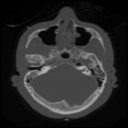
\includegraphics[width=1\linewidth]{images/VisMale_slice.jpg}
%		\caption{A sliced image of the data set}
%		\label{fig:VisMale_slice}
%	\end{minipage}~
%	\begin{minipage}{0.25\textwidth}
%		\centering
%		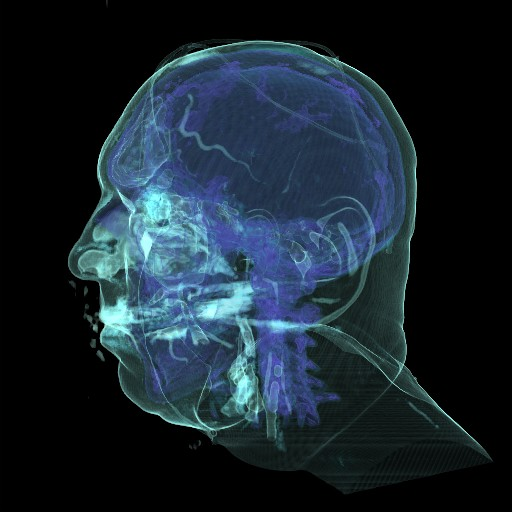
\includegraphics[width=1\linewidth]{images/VisMale.jpg}
%		\caption{Volume rendering of the data set}
%		\label{fig:VisMale}
%	\end{minipage}
%	\caption{The VisMale data set \cite{website:Roettger_volume_2013}}
%	\label{fig:multiple_VisMale}
%\end{figure}

Traditionally, volume rendering techniques are categorized as direct volume rendering and indirect volume rendering.
Indirect volume rendering is done be extracting surfaces from the data sets and rendering these surfaces, while direct volume rendering render the volume data set as a complete block of data without extracting intermediary structures.
Since indirect volume rendering is not in the scope of this thesis, direct volume rendering would henceforth be referred to as volume rendering.

Volume visualization is another term for volume rendering, sometimes with emphasis on the realistic aspects of volume rendering. In addition to the realistic aspects of volume rendering, there is non-photorealistic volume rendering, which emphasizes the illustrative and artistic aspects of volume rendering.
Volume visualization was initially used in medical imaging, and later became an essential techinque in many sciences for portraying complex phenomena such as clouds, water flows, and molecular and biological structure \cite{rosenblum_scientific_1994}.

\begin{figure}
\centering
\begin{minipage}{.25\textwidth}
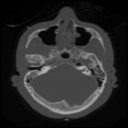
\includegraphics[width=1\linewidth]{images/VisMale_slice.jpg}
\caption{A sliced image of the data set}
\label{fig:VisMale_slice}
\end{minipage}~
\begin{minipage}{.25\textwidth}
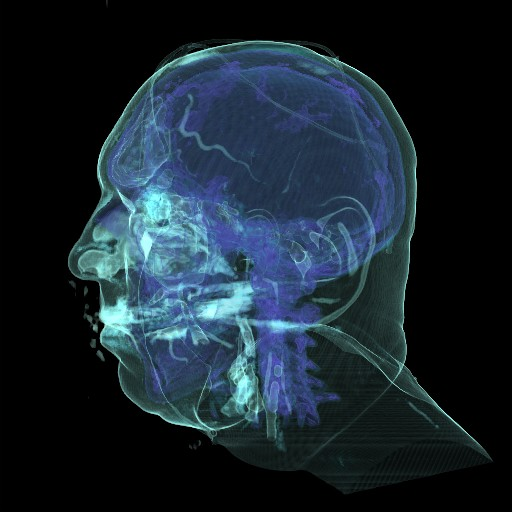
\includegraphics[width=1\linewidth]{images/VisMale.jpg}
\caption{Volume rendering of the data set}
\label{fig:VisMale}
\end{minipage}
\caption{The VisMale data set \cite{website:Roettger_volume_2013}}
\label{fig:multiple_VisMale}
\end{figure}

%Whereas rendering from polygonal representations extracted from volumetric data sets is also called indirect volume rendering.

%There are four typical volume rendering techniques: ray casting, splatting, shear warp and texture mapping. In recent years, many variants and combinations of these techniques have been proposed, especially approaches which utilise GPU hardware to improve performance or even achieve real-time interactivity.

%A volume renderer maps every voxel (an element in volume data) to an opacity and a color with a transfer function, which is a piecewise linear function or an arbitrary table. Once converted to an RGBA value, the composed RGBA result is projected on corresponding pixel of the frame buffer with certain volume rendering techniques.

\subsubsection{Non-Photorealistic Rendering (NPR)}
In contrast to traditional computer graphics, which has focused largely on creating photorealistic images of synthetic objects, non-photorealistic rendering (NPR) is an area of computer graphics that focuses on creating abstract images with a wide variety of expressive styles \cite{haeberli_paint_1990}. NPR has been an active research area for a long time. A number of approaches have been proposed to produce convincing artistic styles for both off-line and on-line rendering. For example, there are various types of commonly used styles including painterly rendering, edge stylization, sketch-shading, cel-shading, hatching.
% Although there are plenty of works on non-photorealistic rendering, most of them focus on how to imitate artistic styles with emphasis on aesthetic aspects.
%Researchers in modelling and rendering in computer graphics have focused for many years on producing photorealistic images, which are indistinguishable from photographs captured from real-world scene. Nevertheless, there are other compelling methods of visual discourse such as paintings, sketches and cel animation.
In certain situations, non-photorealistic renderings are considered more effective and expressive than an equivalent photograph \cite{healey_perceptually_2004}.

%As a basic part of most approaches to non-photorealistic volume rendering, contours delineate object shape and clarify sites of occlusion by emphasizing the transition between front-face and back-facing surface locations.
%Kindlmann et al. \cite{kindlmann_curvature-based_2003} proposed curvature-based transfer function to enhance the expressive and informative power of volume rendering. In their approach, volume data is rendered with contours to exhibit constant thickness in image space.

\subsubsection{Illustrative Volume Visualization}
NPR models were adopted in visualization and hence formed the field illustrative visualization.
Illustrative visualization, as a novel category of visualization, aims at visualizing data in a clear and understandable way using techniques from traditional hand-crafted illustrations.
Illustrative visualization has been successful employed in medical visualization \cite{svakhine_illustration_2005} \cite{viola_importance-driven_2005} \cite{svakhine_illustration-inspired_2009}.

Illustration-based styles are believed to be effective in conveying information. Researchers in the field of computer graphics and visualization have applied illustration-based styles in order to produce effective and expressive visualization. Stompel et al. \cite{stompel_visualization_2002} introduced feature enhancement techniques, such as strokes based, temporal domain enhancement, to enhance time-varying data obtained from the field of computational fluid dynamics (CFD).

In scientific visualization, features of interest are often inner structures of the data sets, e.g. visualizing certain structures in anatomical data sets \cite{diaz_iriberri_enhanced_2013}.
Inspired by techniques from illustration, various approaches are proposed to reveal different level of structures simultaneously in volume data sets.
Two level rendering \cite{hauser_two-level_2001} \cite{hadwiger_high-quality_2003} \cite{corcoran_perceptual_2010} is a method of merging several volume rendering techniques into a single rendering. This method is useful when inner structures needs to be rendered along with semitransparent outer parts.
Focus and context \cite{wang_magic_2005} \cite{bruckner_illustrative_2006} \cite{chen_intelligent_2008} provides a means of revealing the interior of a volume data set in a feature-driven way and also retaining context information.
Another alternative is the cutaway technique \cite{burns_feature_2007} \cite{sigg_intelligent_2012}, which makes inner structures clearly visible along with its spatial relation to the surrounding material.

\subsubsection{Other NPR Techniques in Volume Visuailzation \label{painterly_rendering}}
Streamlines and textures are often used to represent flow directions \cite{urnessy_techniques_2004}. Interrante and Grosch \cite{interrante_strategies_1997} introduced volume LIC (Line Integral Convolution) to visualize 3D flow via volume textures.
%Figure~\ref{fig:interrante_strategies_1997} shows a volume texture generated with LIC. In this figure, vorticity magnitude is mapped to streamline color and the striations along the axial direction reveal the presence of periodic waves propagated down the jet axis.
Since volume LIC is limited to steady flows, Liu and Moorhead \cite{liu_texture-based_2005} introduced an accelerated unsteady flow LIC algorithm to generate volume flow textures.
% (Figure~\ref{fig:liu_texture-based_2005}).
In their approach, magnitude-based transfer functions and cutting planes in volume rendering are employed to show the flow structure and the flow evolution.

Artists recognize patterns and flows in a target scene and express them through brush strokes. They use stroke orientation corresponding to the actual movement \cite{lee_motion_2009}. This type of techniques from master painting and human perception are used to visualize multidimensional data sets \cite{healey_perceptually_2004}. Tateosian et al. \cite{tateosian_engaging_2007} use the color, orientation and size of strokes to represent the magnitude, flow orientation and pressure of a 2D slice of a simulated supernova collapse.
% (Figure~\ref{fig:tateosian_engaging_2007}).
Lee et at. \cite{lee_motion_2009} presented a painterly rendering technique based on the motion information (magnitude, direction, standard deviation) extracted from an image sequences of the same view.
Besides stroke-based techniques and texture-based techniques, particle-based techniques \cite{busking_particle-based_2007} \cite{van_pelt_illustrative_2010} were also proposed to produce user-configurable stylized renderings from volume data sets, imitating traditional pen and ink drawings.

%\begin{figure}
%	\centering
%	\begin{minipage}{.49\textwidth}
%		\centering
%		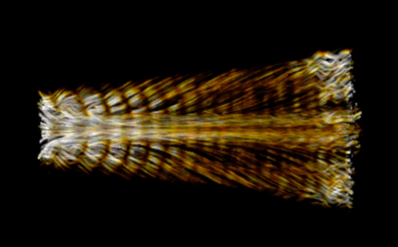
\includegraphics[width=1\linewidth]{images/interrante_strategies_1997.png}
%		\caption{Streamlines are represented as a volume texture, which provides an intuitive impression of the 3D flow. \cite{interrante_strategies_1997}}
%		\label{fig:interrante_strategies_1997}
%	\end{minipage}~
%	\begin{minipage}{.49\textwidth}
%		\centering
%		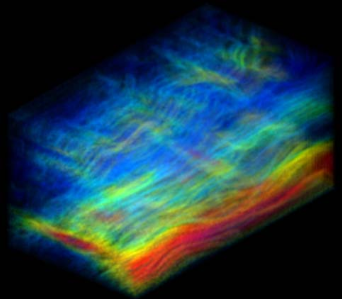
\includegraphics[width=1\linewidth]{images/liu_texture-based_2005.png}
%		\caption{Streamlines are represented as a volume texture, which provides an intuitive impression of the 3D flow. \cite{liu_texture-based_2005}}
%		\label{fig:liu_texture-based_2005}
%	\end{minipage}
%\end{figure}
%
%\begin{figure}
%	\centering
%	\begin{minipage}{.49\textwidth}
%		\centering
%		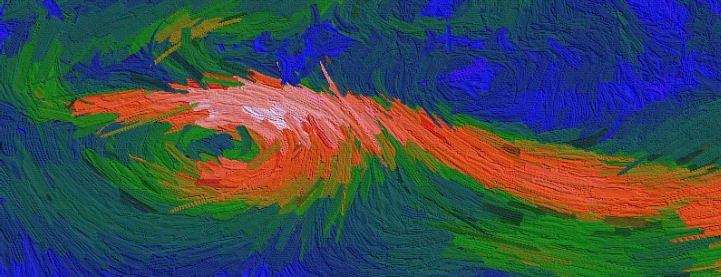
\includegraphics[width=1\linewidth]{images/tateosian_engaging_2007.png}
%		\caption{A visual complexity style visualization of flow patterns in a 2D slice though a simulated supernova collapse, using the mappings: flow orientation $ \rightarrow $ stroke orientation, magnitude $ \rightarrow $ order and pressure $ \rightarrow $ stroke size \cite{tateosian_engaging_2007}.}
%		\label{fig:tateosian_engaging_2007}
%	\end{minipage}~
%	\begin{minipage}{.49\textwidth}
%		\centering
%		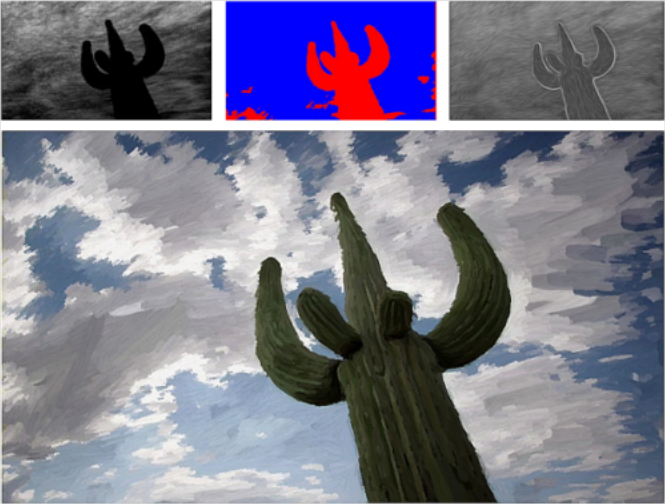
\includegraphics[width=1\linewidth]{images/lee_motion_2009.png}
%		\caption{The motion directions determine stroke orientations in the regions with significant motions, and image gradients determine stroke orientations where little motion is observed \cite{lee_motion_2009}.}
%		\label{fig:lee_motion_2009}
%	\end{minipage}
%\end{figure}

\section{Transfer Functions \label{literature_of_transfer_function}}
Volume data are 3D entities with information inside them, but the data might not consist of surfaces and edges.
%, or might be too voluminous to be represented geometrically.
%The goal of volume visualization is to gain insightful depictions of volume data.
Because of the lack of explicit geometric information, %and limited semantics, 
it is a major challenge to provide clear visualizations of the structures contained in a volume dataset.
Volume data may be rendered directly by mapping scalar values to visual properties (e.g. opacity and color), or an intermediate geometric representation may be extracted using techniques like Marching Cubes \cite{lorensen_marching_1987} and then rendered as geometric surfaces. The mapping, which assigns visual properties to volume data, is called a transfer function.

Transfer function specification is an essential part in volume visualization.
%In terms of dimensionality, transfer functions are divided into two categories, one-dimensional (1D) and multidimensional.
A simple one-dimensional transfer function is a mapping from scalar values to RGB and alpha values.
The resulting visualization largely depends on how well the transfer function captures features of interest \cite{kniss_multidimensional_2002}.
%Due to the complex nature of volumetric data sets, abstraction techniques is often used in order to provide better understanding of the data sets.
However, it is non-trivial to obtain an effective transfer function. The specification is often a trial-and-error process, which involves a significant amount of tweaking of color and opacity. Figure~\ref{fig:multiple_glk_transfunction} shows how slight changes in the transfer function lead to significant changes in the resulting images. The adjustment of transfer functions is unintuitive and often difficult.

\begin{figure}
        \centering
        \begin{minipage}{0.5\textwidth}
                \centering
                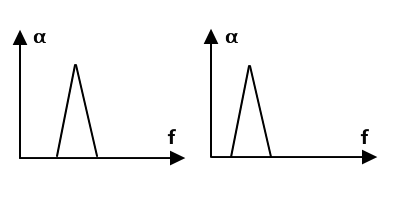
\includegraphics[width=1\linewidth]{images/glk_transfunction_tf.png}
                \caption{Two transfer functions (TF)}
                \label{fig:glk_transfunction_tf}
        \end{minipage}~
        \begin{minipage}{0.25\textwidth}
                \centering
                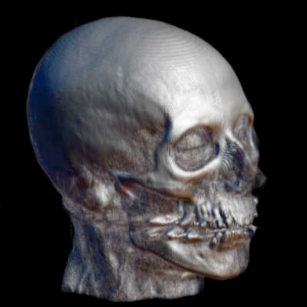
\includegraphics[width=1\linewidth]{images/glk_transfunction_1.png}
                \caption{The result from the TF on the left in \ref{fig:glk_transfunction_tf}}
                \label{fig:glk_transfunction_1}
        \end{minipage}~
        ~ %add desired spacing between images, e. g. ~, \quad, \qquad etc.
          %(or a blank line to force the subfigure onto a new line)        
        \begin{minipage}{0.25\textwidth}
                \centering
                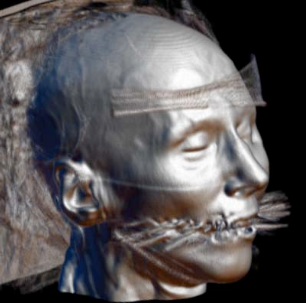
\includegraphics[width=1\linewidth]{images/glk_transfunction_2.png}
                \caption{The result from the TF on the right in \ref{fig:glk_transfunction_tf}}
                \label{fig:glk_transfunction_2}
        \end{minipage}    
        \caption{Slight changes in the transfer function causes significant difference in the resulting images \cite{kindlmann_transfer_2002}}
        \label{fig:multiple_glk_transfunction}
\end{figure}

In practice, major factors that have a great influence on transfer function setting are: partial volume effect \footnote{During the acquisition of data, the finite resolution causes contributions of different materials combined into the value of a single voxel. This is generally referred to as the partial volume effect, which results in blurred boundaries and hampers the detection of small or thin structures. \cite{serlie_classifying_2007}}, non-uniform distribution of materials and noise \cite{serlie_computed_2003}.
Among these, two challenging problems that need to be tackled could be elaborated as follows: firstly, for volume data sets, e.g. those obtained by MRI and CT, different tissues are represented in similar or even overlapping ranges of scalar values; secondly, interesting interior structures are often partly or completely occluded by surrounding tissue.
%This is common in visualizing interior structures. 
Consequently, feature detection and understanding volume data become a big challenge.

These problems are handled by transfer functions, which have played a crucial role in volume visualization.
%Transfer functions have played a crucial role in volume visualization.
Good transfer functions reveal important structures in the data without obscuring them with less important regions.
%Traditional one-dimensional transfer function approaches, which assign optical properties only based on scalar value, are inadequate to extract inner structures of interest from volume data.
%Various strategies have been proposed to simplify transfer function specification \cite{pfister_transfer_2001}.
The design of transfer functions to generate informative visualizations has been a significant challenge addressed by a number of researchers \cite{pfister_transfer_2001}.
Various strategies have been proposed for transfer function design \cite{hadwiger_real-time_2006}.
%Data-centric strategies examine the properties of volume data sets.
Data-centric strategies examine the properties of volume data sets.
However, certain features are difficult to be extracted and visualized with 1D transfer functions, e.g. CT and MRI data sets which contain complex boundaries between multiple materials.
Overlapping intensity intervals corresponding to different materials make boundary separation difficult.
When one intensity value or interval is associated with multiple boundaries, a 1D transfer function is unable to render them in isolation \cite{kniss_multidimensional_2002}.
%Overlapping intensity intervals corresponding to different materials make boundary detection difficult.
%However, certain features of interest in volume data are difficult to extract and visualize with 1D transfer functions. For instance, many medical data sets created from CT or MRI scans contain a complex combination of boundaries between multiple materials. This situation is problematic for 1D transfer functions because of the potential for overlap between the data value intervals spanned by the different boundaries. When one data value or data range is associated with multiple boundaries, a 1D transfer function is unable to render them in isolation \cite{kniss_multidimensional_2002}.

Classical approaches to this problem try to detect boundary information between tissues by introducing derived attributes such as first and second-order derivatives to isolate materials \cite{kindlmann_semi-automatic_1998} \cite{kniss_multidimensional_2002}. In this case, the transfer functions are extended to multidimensional feature spaces. 
The introduction of multidimensional transfer functions alleviates the material separation problem.
Instead of classifying a voxel based on a single scalar value, multidimensional transfer functions allow a voxel to be classified based on a combination of values.
Multidimensional transfer functions are very effective means to extract materials and their boundaries for both scalar and multivariate data.
In addition, various user interfaces were proposed to simply the design of multidimensional transfer functions \cite{tzeng_novel_2003} \cite{tzeng_cluster-space_2004}.
However, the parameter spaces of multidimensional transfer functions are more complex (compared to 1D transfer functions) and thus introduce problems such as requirement for large amount of user interaction, missing precision or the interaction being complex and unintuitive \cite{arens_survey_2010}.
%As a result, the interaction of transfer functions becomes more complex and unintuitive.

There are other multidimensional transfer functions approaches, such as spatialized gradient-based transfer functions \cite{roettger_spatialized_2005}, distance-based transfer functions \cite{tappenbeck_distance-based_2006}, size-based transfer function \cite{correa_size-based_2008}, texture-based transfer functions \cite{caban_texture-based_2008} \cite{alper_selver_exploring_2015} and curvature based transfer functions \cite{kindlmann_curvature-based_2003}.
Bruckner and Gr{\"o}ller introduced the concept of style transfer functions \cite{bruckner_style_2007}, which aim to produce more comprehensible images by using transfer functions that map input values to different NPR rendering styles.

Another strategy is based on the selection of rendered images. This strategy lets the user select one or more favorite images to guide the further search of transfer functions \cite{marks_design_1997} \cite{wu_interactive_2007}. More recent approaches introduced visibility \cite{correa_visibility-driven_2009} \cite{correa_visibility_2011} or measures derived from information theory \cite{haidacher_information-based_2008} \cite{bruckner_isosurface_2010} \cite{ruiz_automatic_2011} \cite{bramon_information_2013}. Zhou et al. \cite{zhou_transfer_2012} studied the combination of 2D transfer functions with occlusion and size-based transfer functions.

Despite the advances of these methods, transfer function design for volume rendering is still an open research problem.
The creation of transfer functions needs to be simplified and the functionality of transfer functions needs to be extended in order to realize the full potential of volume rendering. For instance, more sophisticated transfer functions are required in medical imaging, in order to address various domain specific visualization problems \cite{lindholm_spatial_2010}.

Moreover, transfer function specification in general is an unintuitive or even monotonous task for average users, because it is usually an iterative process of trial and error.
For instance, there are skin and fat tissues around the brain, and their intensities lie in the same range as the brain. If we want to visualize the brain by setting the scalar value range of the brain to opaque, the surrounding skin and fat tissue will also become opaque. Then the brain will be occluded by the surrounding soft tissues which make it difficult to explore the brain structure.
Common approaches to this problem are to introduce explicit segmentation of structures of interest before the volume rendering process \cite{rezk-salama_opacity_2006}. In fact, the process of applying the transfer function could be interpreted as a segmentation problem.

\subsection{Multidimensional Transfer Functions}
Multidimensional transfer functions \cite{kniss_interactive_2001}, which are mappings from intensity and other variables, such as first and second derivatives to color and opacity, have demonstrated their effectiveness in distinguishing boundaries between materials in volume data.

%Overlapping intensity intervals corresponding to different materials make boundary detection difficult. Classical approaches try to detect boundary information between tissues by introducing derived attributes such as first and second derivatives to isolate materials \cite{kindlmann_semi-automatic_1998} \cite{kniss_multidimensional_2002} \cite{kindlmann_transfer_2002}.
%In this case, the transfer functions are extended to multidimensional feature spaces. As a result, the interaction of transfer functions becomes more complex and unintuitive as the dimensionality becomes higher.
%%Even two-dimensional transfer functions require a considerable amount of user interaction to find a meaningful shape \cite{arens_survey_2010}.

In volume data, boundaries are regions between areas of relatively homogeneous material. It is difficult to detect boundaries because different materials often consist of overlapping intensity intervals. To address this problem, multidimensional transfer functions used derived attributes such as gradient magnitudes and second derivatives along with scalar values, in order to detect transitions between relatively homogeneous areas \cite{kindlmann_semi-automatic_1998} \cite{kindlmann_transfer_2002}.
%Classical approaches try to detect boundary information between tissues by introducing derived attributes such as first and second derivatives to isolate materials \cite{kindlmann_semi-automatic_1998} \cite{kniss_multidimensional_2002} \cite{kindlmann_transfer_2002}.
%and exploration of the transfer function domain might not be intuitive.
%As a result, the interaction of transfer functions becomes more complex and unintuitive as the dimensionality becomes higher.
In this case, the transfer functions are extended to multidimensional feature spaces.
For higher-dimensional transfer functions, the generation of transfer functions could be memory intensive and costly to compute, and the interaction of transfer functions are more complex and unintuitive as the dimensionality becomes higher. 

Therefore, two-dimensional (2D) histograms are often used in multidimensional transfer functions \cite{maciejewski_structuring_2009}. An example is a 2D histogram with axes representing a subset of the feature space (e.g. scalar value vs gradient magnitude), with each entry in the 2D histogram being the number of voxels for a given feature space pair.
Even in the case of two-dimensional transfer functions, a considerable amount of user interaction is required in order to come up with meaningful results \cite{arens_survey_2010}.
%A great number of transfer function approaches have also been merged and one-dimensional transfer function is extended to multi-dimensional transfer function.
%Even in the case of two-dimensional transfer functions, a considerable amount of user interaction is required in order to come up with meaningful results \cite{arens_survey_2010}.
%There are other multi-dimensional transfer functions approaches, such as spatialized gradient-based transfer functions \cite{roettger_spatialized_2005}, distance-based transfer functions \cite{tappenbeck_distance-based_2006}, size-based transfer function \cite{correa_size-based_2008}, texture-based transfer functions \cite{caban_texture-based_2008} and curvature based transfer functions \cite{kindlmann_curvature-based_2003}.

As one of the most common representations of voxel distributions, histograms are used in transfer function design to assign visual properties to voxels \cite{pfister_transfer_2001}. Bajaj et al. \cite{bajaj_contour_1997} introduced the contour spectrum to determine voxels corresponding to important isosurfaces in the volume. To overcome the difficulty of using one-dimensional transfer functions (solely based on scalar values stored in the voxels) to extract inner structures of interest from the volume data, Levoy \cite{levoy_display_1988} proposed the use of gradient magnitude to emphasize strong boundaries between different tissues.

The introduction of gradient magnitude as a data metric aims to detect voxels that are of large deviation compared with other voxels by approximating gradient magnitude at each sample point in the volume, because the exact distribution of data is unknown due to information lost in the discrete sampling process.
Kindlmann and Durkin \cite{kindlmann_semi-automatic_1998} extended Levoy's work \cite{levoy_display_1988} by introducing a higher dimensional transfer function domain based on gradient magnitudes and second derivatives. To emphasize different structures, Kniss et al. \cite{kniss_interactive_2001} presented a technique for interactively manipulating 2D histograms of gradient magnitudes and data values. In their work, material boundaries appear as arcs in the 2D histogram and can be selected with interactive widgets \cite{kniss_multidimensional_2002}.
Kindlmann et al. \cite{kindlmann_curvature-based_2003} proposed curvature-based transfer function to enhance the expressive and informative power of volume rendering. In their approach, volume data is rendered with contours to exhibit constant thickness in image space.

{\v S}ereda et al. \cite{sereda_visualization_2006} proposed LH histograms for improving the identification and selection of boundaries in 2D intensity-gradient transfer functions. Subsequently, they \cite{sereda_automating_2006} presented a clustering method based on the LH histograms for semi-automatic transfer function design.
Haidacher et al. \cite{haidacher_volume_2010} described the statistical transfer function space, which is based on statistical properties such as mean and standard deviation of the data values (e.g. intensity and gradient magnitude for 2D transfer functions) in the neighborhood of each voxel. This approach can reduce the influence of noise and enhance visual appearance in volume rendering.

Wang et al. \cite{wang_automating_2012} described a clustering approach on 2D density plots for automatic transfer function design. Their approach allows the user to interactively explore the pre-computed clusters in the feature space and merge or remove uninterested features to improve visualization quality.
Ip et al. \cite{ip_hierarchical_2012} described a multilevel segmentation technique that mimics user exploration behaviors by recursively segmenting intensity-gradient histograms.

In addition, parallel coordinates and dimensionality reduction algorithms (e.g. principal component analysis) were employed to support the design of transfer functions in multidimensional parameter spaces \cite{zhao_multi-dimensional_2010} \cite{guo_multi-dimensional_2011} \cite{kim_dimensionality_2010}.

\subsection{Transfer Functions for Time-Varying Volume Visualization}
Although researchers have developed a great number of visualization techniques for time-invariant volume data, how to effectively explore and understand time-varying volume data remains a challenging problem. Finding good transfer functions for time-invariant volume data itself has proven difficult \cite{pfister_transfer_2001}.
%Finding good transfer functions for time-varying volume data is even more difficult, as data value ranges and distributions change over time.
%Although researchers have developed a great number of visualization techniques for static volume data, how to effectively explore and understand time-varying volume data remains a challenging problem.
Finding good transfer functions for time-varying volume data is more difficult than for static volume data, as data value ranges and distributions change over time.

Coherence is an important issue of transfer function design for time-varying volume data. Ideally, a single transfer function should be used for the whole time-varying data set in order to obtain coherent visualization. More than one color or opacity map can be misleading or physically meaningless, because the transition from one transfer function to another may cause sudden changes in the resulting images. However, this practice is not always applicable to general time-varying data sets.

Volume data sets are inherently 3D representations. Automated analysis methods, such as temporal trends or statistical aggregates e.g. mean values and standard deviations, are often applied in order to abstract dynamic characteristics of the data sets \cite{kehrer_visualization_2013}.

%Jankun-Kelly and Ma \cite{jankun-kelly_study_2001} examined how to combine transfer functions for different time-steps to generate a coherent transfer function.
Jankun-Kelly and Ma \cite{jankun-kelly_study_2001} examined how to combine transfer functions for different time-steps to generate a coherent transfer function.
Woodring et al. \cite{woodring_high_2003} considered time-varying volume data as four-dimensional data field and provided a user interface to specify hyperplanes in 4D.
Woodring and Shen \cite{woodring_chronovolumes_2003} introduced an alternative approach to render multiple time-steps in a sequence with different colors into a single image. This approach provides the context of surrounding time steps but coherence of color among time-steps is hard to maintain.

Tikhonova et al. \cite{tikhonova_exploratory_2010} presented an exploratory approach based on a compact representation of each time step of the dataset in the form of ray attenuation functions. Ray attenuation functions are subsequently used for transfer function generation.
Akiba et al. \cite{akiba_simultaneous_2006} introduced the time histogram which allows simultaneous classification and specification of temporal transfer functions for the entire time series.

A time-varying volume data set can be considered as a 3D array where each voxel contains a time-activity curve (TAC). Fang et al. \cite{fang_visualization_2007} described an approach for classifying time-varying volume data based on the temporal behavior of voxels and three different similarity measures that can be used in their approach.
Woording and Shen \cite{woodring_multiscale_2009} presented a method that filters time-varying volume data into several time scales using wavelet transform and classifies the voxels by clustering the entire time series by time scale.
Lee and Shen \cite{lee_visualizing_2009} proposed a method for classifying time-varying features using time activity curves with the dynamic time warping distance metric.

A single static transfer function maybe be able to capture dynamic features whose their intensity change over time.
To address this problem, Woodring et al. \cite{woodring_semi-automatic_2009} utilized a method called temporal clustering and sequencing to find dynamic features in value space and create dynamic transfer functions through time-series analysis (Figure~\ref{fig:woodring_semi-automatic_2009}).

\begin{figure}
	\centering
	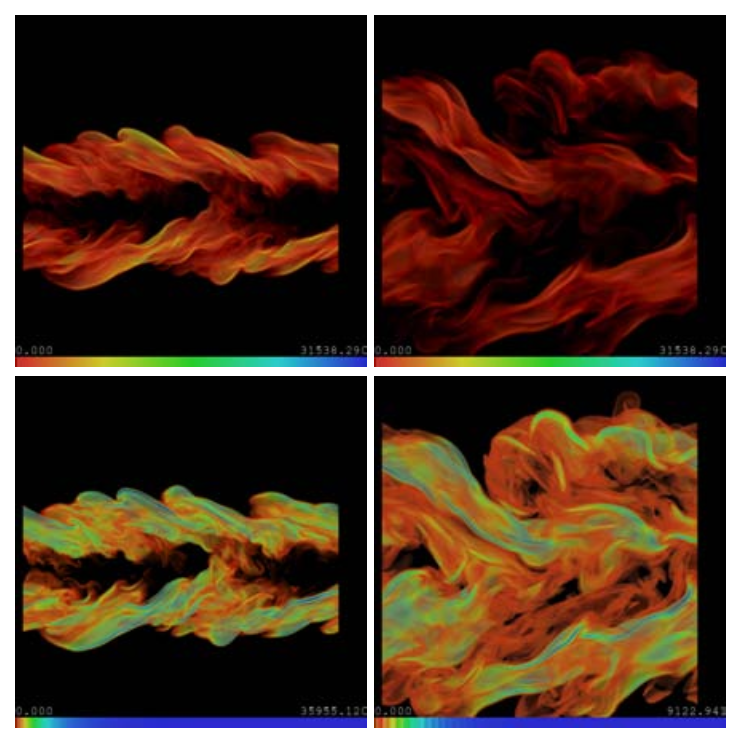
\includegraphics[width=1\linewidth]{images/woodring_semi-automatic_2009}
	\caption{A single static transfer function cannot capture dynamic features. In the two images at the top, the features appear to vanish over time. On the other hand, the features are visible over time if a dynamic transfer function is used (the two images at the bottom) \cite{woodring_semi-automatic_2009}.}
	\label{fig:woodring_semi-automatic_2009}
\end{figure}

Ward and Guo \cite{ward_visual_2011} presented a method for visualizing time-series data that reveals a wide variety of features in the data, by mapping short sub-sequences of the time-varying volume data into a high-dimensional shape space, and then performing a dimension reduction process to allow projection into screen space.

Gu and Wang \cite{gu_transgraph:_2011} proposed an approach to organize a time-varying data set into a hierarchical graph, which captures the transition relationships in the data set. This approach assists the user in comprehending the correspondence between volume regions over time and allows interaction of the graph through brushing and liking.

In order to create coherent and feature-prominent animations of time-varying volume data, Peng et al. \cite{peng_optimal_2011} described an optimal color mapping strategy, which uses a two-phase optimization method with bilateral filtering and energy minimization.

\subsubsection{Visualising Time-Varying Volume Data with NPR}
An essential problem in time-varying volume visualization is to visualize temporal variation and analysis of features. Traditionally, time-varying data has been visualized as snapshots of individual time steps or animation of snapshots of a sequence of time steps. These techniques are effective in making time-varying data understandable. However, they struggle when the complexity of data sets increased dramatically in recent years \cite{brambilla_illustrative_2012}.

Compared to flow visualization, which is a well established branch of scientific visualization \cite{brambilla_illustrative_2012}, general time-varying volume visualization is still a relative young field.
Illustrations for time-varying rendering could be divided into two categories, one is to enhance time-invariant features and the other is to enhance temporal features of time-varying volume data. The techniques in the first category focus on enhancing structural perception of volume models through the amplification of features and the addition of illumination effects \cite{rheingans_volume_2001} \cite{joshi_illustration-inspired_2005}. Examples of these techniques include boundary enhancement, oriented feature enhancement (silhouettes, fading, and sketch lines). The techniques in the second category focus on illustrating dynamic aspects such as movement of features. A few kinds of techniques have been proposed for this purpose. For example, there are speed lines, flow ribbons and strobe silhouettes, which are inspired by traditional animation \cite{joshi_illustration-inspired_2005} \cite{joshi_evaluation_2008} \cite{joshi_case_2009}; and there are extended silhouette and boundary enhancement domains, which are inspired by the techniques used by illustrators and other artists \cite{svakhine_illustration_2005}. Nevertheless, illustrations of temporal features of time-varying data requires more attention from researchers in the visualization community. The usefulness of illustrative approaches in time-varying volume visualization has not been studied as thoroughly as in other areas.

\section{Automated Transfer Function Generation}
Researches have proposed various approaches to automate the design of transfer functions and provide acceptable suggestions which can be further edited by users. However, the usefulness of a transfer function mostly depends on the underlying question the user wants to answer. Moreover, users' tasks vary drastically from one domain to another. Therefore, most techniques work semi-automatically and very few techniques consider domain knowledge in the design process \cite{zudilova-seinstra_trends_2008}.

He et al. \cite{he_generation_1996} addressed transfer function exploration as a parameter optimization problem and presented an approach to assist the user in exploring appropriate transfer functions using stochastic search techniques starting from an initial population.
Another strategy is further tuning transfer functions based on user selection of favorable rendered images as feedback, in order to achieve desired results.
Marks et al. \cite{marks_design_1997} presented Design Gallery, which lets the user select one or more favorite images to guide the further search of transfer functions.
Rezk-Salama et al. \cite{rezk-salama_automatic_2000} presented high-level semantics to abstract parametric models of transfer functions in order to automatically assign transfer function templates.

%\cite{jani_opacity_2005}
Wu and Qu \cite{wu_interactive_2007} developed a method that uses editing operations and stochastic search of the transfer function parameters to maximize the similarity between volume-rendered images given by the user.
Maciejewski et al. \cite{maciejewski_structuring_2009} described a method to structure attribute space in order to guide users to regions of interest within the transfer function histogram.
Chan et al. \cite{chan_perception-based_2009} developed a system to optimize transparency automatically in volume rendering based on Metelli\rq s episcotister model to improve the perceptual quality of transparent structures.
Correa and Ma \cite{correa_visibility-driven_2009} proposed the visibility histogram to guide the transfer function design.

Zhou and Takatsuka \cite{zhou_automatic_2009} presented an automated approach for generating transfer functions, which can depict inclusion relationship between structures in the volume, and maximize opacity and color differences among the structures. This approach uses a residue flow model based on Darcy\rq s Law to differentiate the distribution of opacity between branches of a contour tree.
Selver and G{\"u}zeli{\c s} \cite{alper_selver_semiautomatic_2009} introduced a semi-automatic method for transfer function initialization and optimization using volume histogram stacks and radial basis function networks.

Want et al. \cite{wang_efficient_volume_2011} extended visibility histograms to feature visibility, in order to measure the influence of each feature to the volume rendered image. Their approach allows the user to directly specify the desired visibility for the features of interest, and the appropriate opacity values are automatically obtained. This mechanism is similar to the perception-based transparency equalization \cite{chan_perception-based_2009}, which automatically optimize the rendering parameters based on psychological principles, in order to deliver results complying with viewer's perception.

Inspired by how physicians interact with volume data to extract clinically relevant information, L{\"a}th{\'e}n et al. \cite{lathen_automatic_2012} proposed an optimization method for shifting transfer function presets, in order to better visualize contrast enhanced blood vessels.
%Automatic Tuning of Spatially Varying Transfer Functions for Blood Vessel Visualization

%\cite{woo_feature-driven_2012}
%%Feature-driven data exploration for volumetric rendering
%\cite{jung_opacity-driven_2014}
%%Opacity-driven volume clipping for slice of interest (SOI) visualisation of multi-modality PET-CT volumes

Maciejewski et al. proposed a non-parametric method to generate transfer function \cite{maciejewski_structuring_2009}.
In their later work \cite{maciejewski_abstracting_2013}, instead of using the attributes, metrics representing relationships and correlations in the underlying data were used in the method.

%A number of approaches have been proposed to automate the design of transfer functions.
%Wu and Qu \cite{wu_interactive_2007} developed a method that uses editing operations and stochastic search of the transfer function parameters to maximize the similarity between volume-rendered images given by the user.
%Maciejewski et al. \cite{maciejewski_structuring_2009} described a method to structure attribute space in order to guide users to regions of interest within the transfer function histogram.
%Chan et al. \cite{chan_perception-based_2009} developed a system to optimize transparency automatically in volume rendering based on Metelli's episcotister model to improve the perceptual quality of transparent structures.
%Correa and Ma \cite{correa_visibility-driven_2009} proposed the visibility histogram to guide the transfer function design.

\section{Visibility Histograms and Visibility-Driven Transfer Functions}
Visibility has been studied in measuring viewpoint quality \cite{bordoloi_view_2005} and enhancing ghost and cutaway views \cite{viola_importance-driven_2004} in volume visualization.
%\cite{bordoloi_view_2005}
%\cite{takahashi_feature-driven_2005}

In traditional transfer function design, the visibility of structures revealed in volume rendering is a consequence of adjusting transfer function parameters, rather than a design parameter \cite{preim_visual_2013}.
Correa and Ma \cite{correa_visibility-driven_2009} introduced visibility histograms to guide transfer function design for both manual and automatic adjustment.
Visibility histograms (Figure~\ref{fig:correa_visibility-driven_2009}), which summarize the distribution of visibility of voxels from a given viewpoint, is a powerful feedback mechanism of volume visualization \cite{emsenhuber_visibility_2008}.
Visibility histograms encode the information required to measure the efficacy of transfer functions and are advantageous in guiding and automating the manipulation of transfer functions.

\begin{figure}
	\centering
	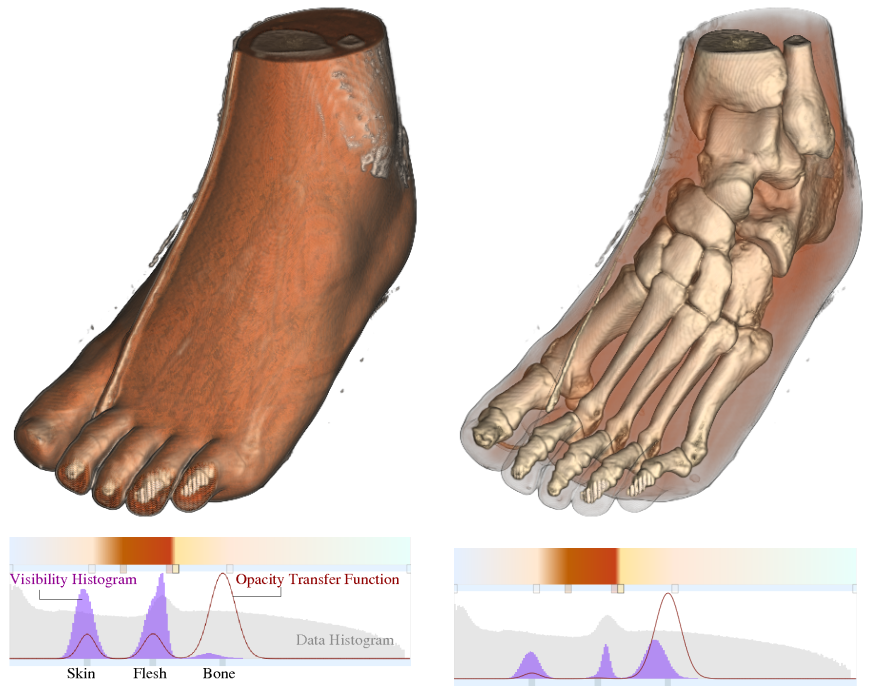
\includegraphics[width=1\linewidth]{images/correa_visibility-driven_2009}
	\caption{Visibility histograms for two data sets \cite{correa_visibility-driven_2009}}
	\label{fig:correa_visibility-driven_2009}
\end{figure}

Want et al. \cite{wang_efficient_2011} extended visibility histograms to feature visibility, in order to measures the influence of each feature to the resulting images. As shown in Figure~\ref{fig:wang_efficient_2011}, they described a scheme that allows user to specify desired visibility for features of interest and subsequently the opacity transfer function is optimized using an active set algorithm \cite{polyak_conjugate_1969}.

\begin{figure}
	\centering
	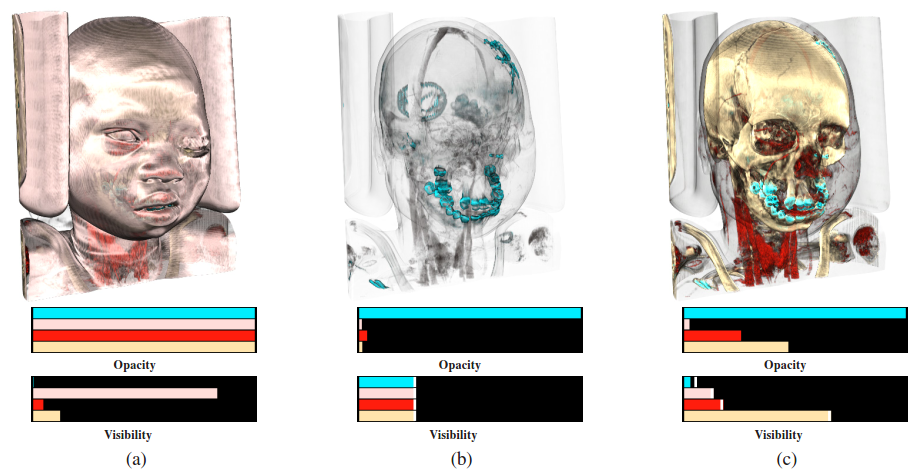
\includegraphics[width=1\linewidth]{images/wang_efficient_2011}
	\caption{Visibility based opacity specification for a CT facial deformity data set \cite{wang_efficient_2011}}
	\label{fig:wang_efficient_2011}
\end{figure}

\cite{mak_visibility-aware_2011}
%Visibility-Aware Direct Volume Rendering

\cite{bronstad_visibility_2012}
%Visibility driven visualization of 3D cardiac ultrasound data on the GPU

\cite{ruiz_automatic_2011}
%Automatic Transfer Functions Based on Informational Divergence

\cite{bramon_information_2013}
%Information Theory-Based Automatic Multimodal Transfer Function Design

%\cite{wan_fast_2010}
%%Fast volumetric data exploration with importance-based accumulated transparency modulation

%\cite{tang_depth-based_2011}
%%Depth-Based Feature Enhancement for Volume Visualization

%\cite{zhou_opacity_2014}
%%Opacity modulation based peeling for direct volume rendering

Marchesin et al. \cite{marchesin_per-pixel_2010} introduced a volume rendering technique that manipulates the voxel opacity values in a view-dependent way, in order to enhance visibility of internal structures in the volume data set.

Jung et al. \cite{jung_dual-modal_2012} presented a dual-modal visualization method, which uses visibility metrics to provide visual feedback regarding the occlusion caused by the volume data in one modal on the other modal.
Jung et al. \cite{jung_visibility-driven_2013} extended visibility histograms to multimodal volume visualization.
They demonstrated the use of visibility histograms together with region of interest segmentation was effective in visualizing PET-CT volume data sets.
Instead of computing the visibility of all voxels, Zheng et al. \cite{zheng_visibility_2013} employed local visibility histograms to ensure both the features of interest and contextual information are visible in multimodal volume visualization.

Schlegel and Pajarola \cite{schlegel_visibility-difference_2013} proposed a visibility-difference entropy metric. They presented an automated approach using this metric for generating a set of transfer function candidates with high ratings and are strongly distinct in what they reveal.
Cai et al. \cite{cai_automatic_2013} described a method to derive opacity transfer functions by minimizing the Jensen-Shannon divergence between the observed visibility distribution and a user-defined target distribution. The target distribution can be defined using Gaussian function weighting.

Qin et al. \cite{qin_voxel_2015} presented the voxel visibility model as a quality metric for transfer function design.
The voxel visibility model is a mapping function from data attributes of voxels to their visibility attributes. Instead of specifying transfer functions, this approach allows users to directly adjust the visibility of each voxel, and then the corresponding opacity transfer functions can be obtained by minimizing the distance between the desired voxel visibility distriubtion and the actual voxel visibility distribution.

\section{Multivariate Volume Visualization}
Analyzing multivariate data is an importance and challenging topic in many scientific disciplines. For instance, applications in medicine, engineering and meteorology often require analyzing multivariate data.
However, multivariate volume data sets are usually mapped to a scalar dimension and visualized separately with standard volume rendering techniques.

Kniss and Hansen \cite{kniss_volume_2002} applied volume rendering with multidimensional transfer function to visualize multivariate weather simulations. In their approach, they combined the temperature and humidity as a multivariate field in order to assist the meteorologists in identifying the frontal zones. 

Akiba et al. presented the use of time histogram for simultaneous classification of time-varying data in order to find transfer functions that classify all the time steps of the data set \cite{akiba_simultaneous_2006}.

Woodring and Shen presented a method for the comparison of different data fields through the expression of a volume shader that composes data fields together with set operations \cite{woodring_multi-variate_2006}.

Wang et al. introduced an importance measure based on conditional entropy and categorize temporal behaviors by clustering the importance curves over time \cite{wang_importance-driven_2008}.

Lee and Shen \cite{lee_visualization_2009} extended the Dynamic Time Warping (DTW) approach \cite{lee_visualizing_2009} to SUBDTW, in order to estimate when a trend appears and vanishes in a given time series. They modeled the temporal relationships as a state machine based on the beginning and ending times of the trends.

Khlebnikov et al. \cite{khlebnikov_noise-based_2013} described a novel method that allows simultaneous rendering of multivariate data by redistributing the opacity within a voxel. This method uses procedural texture synthesis \cite{khlebnikov_procedural_2012} for opacity redistribution pattern and is similar in spirit to color weaving.

Data analysis techniques for high dimensional spaces, such as parallel coordinates \cite{akiba_visualizing_2007} \cite{guo_scalable_2012} and principal component analysis \cite{liu_multivariate_2014}, were also investigated for exploring multivariate time-varying data sets.

%\cite{woodring_multi-variate_2006}
%\cite{akiba_visualizing_2007}
%\cite{guo_scalable_2012}
%\cite{liu_multivariate_2014}

\section{Information Theory in Visualization}
Information theory \cite{shannon_mathematical_1948} was originally introduced to study the fundamental limit of reliable transmission of messages through a noisy communication channel. Traditional applications of information theory, such as data compression and data communication, focus on the efficient throughput of a communication channel, whilst visualization focuses on the effectiveness in aiding the perceptual and cognitive process for data understanding and knowledge discovery.

In recent years, there is an emerging direction towards using the principles of information theory to solve challenging problems in scientific visualization \cite{wang_information_2011}. These problems include view selection \cite{bordoloi_view_2005} \cite{takahashi_feature-driven_2005} \cite{feixas_unified_2009}, streamline seeding and selection \cite{xu_information-theoretic_2010} \cite{lee_view_2011}, transfer function for multimodal data \cite{bramon_multimodal_2012}, representative isosurface selection \cite{wang_lod_2006}, time-varying and multivariate data analysis \cite{wang_importance-driven_2008} and information channel between objects and viewpoints \cite{ruiz_viewpoint_2010}.

Chen and J{\"a}nicke \cite{chen_information-theoretic_2010} presented an information-theoretic framework for visualization. They examined the theoretical aspect of information and its relation to data communication and interpret different stages of the visualization pipeline using the taxonomy of information.

Haidacher et at. \cite{haidacher_information-based_2008} proposed an approach of transfer function specification for multi-modal data visualization. They considered the joint occurrence of multiple features from one or multiple variables in order to separate statistical features that only occur in a single variable from those that are present in both.

Want et al. \cite{wang_importance-driven_2008} introduced an approach to characterized the dynamic temporal behaviors of spatial blocks using importance curves, which are based on conditional entropy. Clustering is performed on the importance curves of all the spatial blocks to classify the underlying volume data set.

Ruiz et al. \cite{ruiz_automatic_2011} presented an approach to generate transfer functions from a target distribution provided by the user. Their approach is based on a communication channel between a set of viewpoints and a set of bins of a volume data set, and supports both 1D and 2D transfer functions including the gradient information.

Bramon et al. \cite{bramon_information_2013} proposed an automatic method to visualize multi-modal data by combining several information-theoretic strategies to define colors and opacity values of the multi-modal transfer function.
They set an information channel between two registered input data sets to define the fused color and minimize the informational divergence between the visibility distribution captured by a set of viewpoints and a target distribution proposed by the user to obtain the opacity.

\section{Computational Saliency}
Predicting salient locations has many real world applications, such as navigational assistance, robot control, surveillance systems, object detection and scene understanding \cite{zhao_learning_2013}.
Inspired by mechanisms of the human visual system, various computational models of visual saliency have been proposed to predict gaze allocation \cite{itti_model_1998} \cite{parkhurst_modeling_2002} \cite{harel_graph-based_2006} \cite{chikkerur_what_2010} \cite{mahadevan_spatiotemporal_2010} \cite{duan_visual_2011}.

Lee et al. \cite{lee_mesh_2005} presented mesh saliency, which is defined in a scale-dependent manner using a center-surround operator on Gaussian-weighted mean curvatures. They observed that their approach was able to capture the most visually interesting regions on a mesh.
Kim and Varshney \cite{kim_saliency-guided_2006} introduced the user of center-surround operators to compute saliency fields of volume data. In their user study, they found that their approach was better at eliciting viewer attention than the traditional Gaussian regional enhancement approaches.
Shen et al. \cite{shen_save:_2014} proposed the use of saliency to assist volume exploration. They described a method for inferring interaction position in volume visualization, in order to help users pick focused features conveniently.
Shen et al. \cite{shen_spatiotemporal_2015} described spatiotemporal volume saliency, which extended the saliency field \cite{kim_saliency-guided_2006} to time-varying volume data.

%\cite{kim_mesh_2010}
%\cite{song_mesh_2014}

%A saliency-based enhancement of volume visualization inspired by the center-surround mechanisms of the human
%visual system
%For volume \cite{kim_saliency-guided_2006}
%\cite{kim_saliency-guided_2008}

%saliency assisted
%\cite{wang_saliency-aware_2013}

%\cite{treue_visual_2003}
%\cite{healey_combining_2001}
%\cite{hall_trainable_2004}
%\cite{kadir_saliency_2001}
%\cite{cui_measuring_2006}

\section{Perceptual Evaluation}
Traditional, visualization research has an emphasis on solving problems with modeling and optimization using engineering and mathematics tools.
A recent focus in visualization has become measuring the effectiveness of a proposed method with adequate user studies \cite{giesen_conjoint_2007}.
Due to the complex nature of the data being studied, simply displaying all available information does not adequately meet the demands of domain scientists \cite{anderson_evaluating_2012}.
%Determining the best use of visualization techniques is one of the goals of visualization evaluations.
User studies can be used to evaluate the strengths and weaknesses of visualization methods \cite{christopher_thoughts_2003}.
The evaluation of visualization methods that focus on human factors often employ user studies or expert evaluations to determine their effects on interpretation and usability.

There are a number of different evaluation strategies, such as measuring user performance, accuracy and experience \cite{redmond_influencing_2010}. Laidlaw et al. \cite{laidlaw_quantitative_2001} compared six methods for visualizing 2D vector fields and measured user performance on three flow-related tasks for each of the six methods. They used the evaluation results to identify what makes a 2D vector fields visualization effective.
Joshi and Rheingans \cite{joshi_evaluation_2008} evaluated the effective of their illustrative techniques by measuring user accuracy, time required to perform a task and user confidence.

Lu \cite{lu_volume_2010} described a method for automatically selecting rendering parameters to simplify user interaction and improve usability. Subsequently, a user study was conducted to evaluate the effectiveness of this method. Two data sets were rendered in three styles with three predefined portions of the data sets were highlighted respectively. The users' eye gaze patterns were analyzed to determine if they were able to accurately identify the highlighted areas in the images.

Kersten-Oertel et al. \cite{kersten-oertel_evaluation_2014} presented empirical studies on the effect of six different perceptual cues for enhancing depth. In the user study, the subjects were asked to determine which one of two indicated vessels was closer to them, and were asked to respond as accurately and quickly as possible. Both the percentage of correct answers and response times were analyzed.

Also for depth perception, D{\'i}az et al. \cite{diaz_perceptual_2015} conducted a user study to investigate the impact of well-known volumetric shading models \cite{kniss_model_2003} in stereoscopic desktop-based environments. In the results, the average time spent and average correctness of answers were analyzed.

\section{Feature Tracking}
Feature extraction and tracking is an established technique for the analysis of time-varying data in various research fields, such as video analysis, computer vision and flow visualization \cite{muelder_interactive_2009}.
In time-varying data, features are objects that evolve over time. Feature tracking aims to determine the correspondence between features in successive time steps and describe the evolution of features through time \cite{post_state_2003}.

In practice, feature extraction and tracking are often employed in the exploration and analysis of time-varying volume visualization in order to better understand the dynamic nature of the underlying phenomena \cite{tzeng_intelligent_2005} \cite{woodring_multiscale_2009} \cite{lee_visualizing_2009} \cite{gu_transgraph_2011}.
Feature extraction methods are often based on an analytic description of the feature of interest. Consequently, feature extraction and tracking could become a manual-driven and trial-and-error process in the case that properties cannot be easily defined and are sometimes unknown \cite{ma_machine_2007}.

%%survey
\cite{ma_machine_2007} \cite{wang_information_2008}
%
\cite{caban_texture-based_2007}
%
%%tracking related works
\cite{widanagamaachchi_interactive_2012} \cite{ozer_group_2012}
\cite{hsieh_feature_2013}

\section{Vector Field Visualization}
The visualization of vector fields plays a crucial role in visual interpretation and understand of the underlying flow features and patterns \cite{kuhn_clustering-based_2011} \cite{ma_coherent_2013}. Since flow patterns also exist in time-varying volume data, certain techniques for visualizing vector field could be incorporated into time-varying volume visualization, in order to depict the dynamic aspects of time-varying data.

Line drawings are effective ways to depict complex information with simple means \cite{benard_state_art_2011}. Among vector field visualization techniques, streamline visualization is a simple but common way to convey the structure of 3D vector fields \cite{chen_illustrative_2011}. Streamlines have proven to give expressive visual representation if they are combined with appropriate seeding strategies \cite{annen_vector_2008}. Streamlines intuitively reveal flow patterns by integrating the flow path.

\section{Summary}
We have presented a review of literature in the field of volume visualization.
The review suggests that it is feasible to optimize the parameters of volume visualization based on the information within volume data. Existing research on multidimensional transfer functions, classification of volume data and information theory provides us the foundation to explore and understand how this optimization may be achieved.
%Existing research on the analysis and visualization of time-varying data and flow data gives us valuable information on the study of the dynamic aspect of time-varying volume data.
In particular, the analysis and visualization of time-varying data is a compelling problem due to increasing availability of such data in recent years. Although some work has been published in this area, it is clear that there is compelling work left to be done in optimizing the rendering of such data sets.
The use of NPR techniques can improve the expressiveness of the visualization and thus facilitate better user understanding of data.
Further studies are required in order to better integrate NPR techniques into the visualization pipeline and enhance the expressiveness by exploiting the information within volume data sets.

%-------------------------------------------------------------------------
                                
\chapter{Information-Guided Transfer Function Refinement for Exploring Volume Data \label{transfer_function_refinement}}
Volume visualization is a powerful technique for depicting layered structures in 3D volume data sets. However, it is a major challenge to obtain clear visualizations of a volume with layers clearly revealed.
In particular, the specification of the transfer function is frequently a time-consuming and unintuitive task in volume rendering.
In this chapter, we describe a global optimization and two user-driven refinement methods for modulating transfer functions in order to assist the exploration of volume data.
This optimization is dependent on the distribution of scalar values of the volume data set and is designed to reduce general occlusion and improve the clarity of layers of structures in the resulting images.
The user can explore a volume by interactively specifying different priority intensity ranges and observe which layers of structures are revealed. In addition, we show how the technique can be applied to time-varying volume data sets by adaptively refining the transfer function based on the histogram of each time-step. 
Experimental results on various data sets are presented to demonstrate the effectiveness of our method.

%-------------------------------------------------------------------------
\section{Introduction}
%Volume rendering is the process of depicting information within volume data sets, which usually contain complex structures of various materials or dynamic phenomena. The majority of such datasets are discretely sampled along a three-dimensional grid and contain scalar values usually acquired from imaging devices such as CT or MRI machines. In other cases, such as in flow visualization, the datasets are often generated from simulations and may constitute a 3D vector field or multi-variate data of even higher complexity.
%%Volume data is stored as an array of voxels (a three-dimensional extension of pixels), the atomic entities that contain information such as the density or other properties of a discretised position in 3D space.
%Such datasets are ubiquitous in science, medicine and engineering but are difficult to deal with as the data typically does not consist of surfaces and edges, which are the typical primitives of a 3D graphics pipeline. Because of the lack of explicit geometric information, %and limited semantics, 
%it is a major challenge to provide clear visualizations of the structures contained in a volume dataset.

%A crucial step in volume rendering is transfer function specification.
Transfer functions play an essential role in volume rendering.
Through the assignment of visual properties, including color and opacity, to the volume data being visualized,
transfer functions impact the final rendering of the data set and thus affect which structures will be 
visible to the user.
%However, obtaining an effective transfer function is a non-trivial task, which typically involves a significant amount of tweaking of color and opacity.
However obtaining an effective transfer function is a non-trivial task, which often entails time-consuming tweaking until 
a desired aesthetic quality is achieved in the resulting rendering.
%Multi-dimensional transfer functions were developed to distinguish transitions between tissues by utilizing data properties such as gradient and second derivatives.
%%However, high-dimensional transfer functions require high amount of user interaction and the means of interaction is often unintuitive.
%However, the design of high-dimensional transfer functions is usually a very involved and unituitive process for the user.
Although a number of automatic or semi-automatic approaches have been developed, 
transfer function design remains a challenging problem \cite{pfister_transfer_2001} \cite{arens_survey_2010}.
%In interactive volume rendering systems, users can obtain good transfer functions via trial-and-error modification of visualization parameters, but the process often entails time-consuming tweaking until a desired aesthetic quality is achieved in the resulting rendering.
%In addition to the complex structures contained in volume data, users have differing goals or features of interest depending on their specific tasks. Therefore, it is almost impossible to generate a transfer function that would suit all kinds of visualization tasks. Also, different subsets of the data may occlude each other and thus result in ineffective visualization.

For end users, such as physicians, who may not have much experience in volume rendering and transfer function design, 
a user-friendly approach that allows them to intuitively explore volume data sets is very desirable.
%Automatic approaches cannot produce satisfactory results in every case. On the other hand, exploratory approaches with simple and efficient interaction are preferable.
As fully automatic approaches cannot currently guarantee satisfactory results in every case, 
exploratory approaches with simple and efficient interaction are highly desirable.

%Although a variety of multi-dimensional transfer functions have been proposed, they are rarely used in practice, due to their high amount of user interaction, missing precision or unintuitive way of handling it. In practice, the use of simple 1D transfer functions is still dominant \cite{arens_survey_2010}.
%\begin{figure}
%        \centering
%%        \begin{subfigure}[b]{0.3\textwidth}
%        \begin{minipage}{.24\textwidth}
%                \centering
%                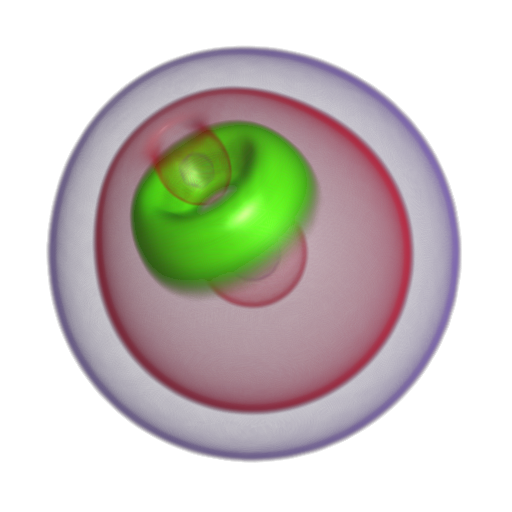
\includegraphics[width=\textwidth]{nucleon.png}
%                \caption{A rendered image with the transfer function in Figure~\ref{fig:tf_nucleon}}
%                \label{fig:nucleon}
%%        \end{subfigure}%
%		\end{minipage}~
%        ~ %add desired spacing between images, e. g. ~, \quad, \qquad etc.
%          %(or a blank line to force the subfigure onto a new line)
%%        \begin{subfigure}[b]{0.3\textwidth}
%        \begin{minipage}{.24\textwidth}
%                \centering
%                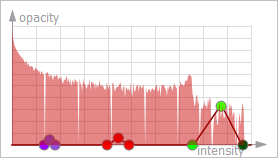
\includegraphics[width=\textwidth]{tf_nucleon.png}
%                \caption{A transfer function with three components. The volume's distribution in logarithmic scale is shown in the background.}
%                \label{fig:tf_nucleon}
%%        \end{subfigure}
%		\end{minipage}
%        \caption{A transfer function and its resulting image of the nucleon data set}\label{fig:multiple_nucleon}
%\end{figure}
%Figure~\ref{fig:tf_nucleon} shows a typical interface for transfer function specification. The control points specify color and opacity for their intensity values. The x-axis is intensity and the y-axis is opacity. Each control point is also assigned a color. The color and opacity of an intensity value is obtained by linear interpolations of the color and opacity of the two adjacent control points. The typical process of transfer function specification involves iterations of assigning colors to control points, moving control points around and then observing the resulting rendered images.
%A rendered image of a nucleon data set is displayed in Figure~\ref{fig:nucleon}. The three components (sets of control points) in Figure~\ref{fig:tf_nucleon} correspond to the three layers in the rendered image.

In this paper, we propose a novel approach to refine the transfer function based on the distribution of the scalar values of the volume data set.
%Our approach provides the ability for users to specify priority intensity ranges in an intuitive way, thus facilitating more interactive exploration of volume data sets.
%This optimization can be done automatically as an initial global optimization with no assumptions of the data set.
Firstly, we propose an automatic step to refine the transfer function that improves the rendering of volume data by reducing overall occlusions with no previous assumptions of the data set. Furthermore, we propose two interactive methods that extend on the optimization technique in order to enhance specific intensity ranges within the data as identified by the user. The process is fast and intuitive and allows the user to provide customized views of the data to aid in visual exploration of the volume data set.

\section{Related Work}
%More recent approaches introduced visibility
%\cite{correa_visibility_2011}
A number of approaches have been proposed to automate the design of transfer functions.
Maciejewski et al. \cite{maciejewski_structuring_2009} described a method to structure attribute space in order to guide users to regions of interest within the transfer function histogram.
Chan et al. \cite{chan_perception-based_2009} developed a system to optimize transparency automatically in volume rendering based on Metelli's episcotister model to improve the perceptual quality of transparent structures.
Correa and Ma \cite{correa_visibility-driven_2009} proposed the visibility histogram to guide the transfer function design. In a later work \cite{correa_visibility_2011}, they generalized the visibility histogram and proposed a semi-automatic method for generating transfer functions by maximizing the visibility of important structures based on the visibility histogram, which represents the contribution of voxels to the resulting image.
Ruiz et al. \cite{ruiz_automatic_2011} also used visibility as a main parameter for the transfer function specification. Their method obtains the opacity transfer function by minimizing the informational divergence between the visibility distribution captured by a set of viewpoints and a target distribution defined by the user. Later, Bramon et al. \cite{bramon_information_2013} extended this approach to deal with multimodal information.

The approach in this paper is based on our previous work% previous work by Luo and Dingliana
\cite{luo_information-guided_2014} on optimizing transfer functions by minimizing the variance of control point weighting, which is generated from the intensity distribution of the data set. User-selected regions are taken into account, in order to enhance priority intensity ranges of importance to the user in the resulting image, and the approach,  in contrast to others discussed previously, is viewpoint-independent.
In this paper, we extend this further by introducing
%In this paper, we present extensions to this work which introduce 
an intensity-based method to facilitate interactive exploration of volume data sets. In addition, we provide a more generalized approach to the distribution of control points, which in the original paper was limited to simplified tent-shaped distributions. Finally, we describe how to propagate optimization of the transfer functions through different time-steps of time-varying data volume sets.
%Recent work on incorporating
%statistical and information metrics into time-varying
%volumetric data includes work by Fang et al. \cite{fang_visualization_2007} on the time
%activity curve, J{\"a}nicke et al. on local statistical complexity
%analysis \cite{janicke_multifield_2007}, and Haidacher et al. \cite{haidacher_information-based_2008} on utilizing information
%theory for fusing traditional transfer function space with
%information enhanced transfer function spaces.

%and measures derived from information theory \cite{haidacher_information-based_2008} 
%\cite{bruckner_isosurface_2010}
%\cite{ruiz_automatic_2011}
%\cite{bramon_information_2013}

%Much of the work in the field of volume visualization has been focused on the synthesis of photorealistic images to assist in the visualization of structures contained in volume data sets.
%However, traditional depictions of the same types of data, such as those found in medical textbooks, deliberately use non-realistic techniques to draw the viewer's attention to important aspects \cite{bruckner_style_2007}. Using abstraction, visual overload is prevented and thus result in a more effective visualization.
%
%Bruckner et al. introduced the concept of style transfer functions \cite{bruckner_style_2007}.
%Techniques from traditional art and illustration are incorporated in the volume rendering process. The goal is to gain clarity compared to photorealism by emphasizing important features, improving data exploration. Less relevant details are omitted and important aspects are highlighted, resulting in more comprehensible images.
%Although researchers have developed a great number of visualization techniques for static volume data, how to effectively explore and understand time-varying volume data remains a challenging problem. Finding good transfer functions for time-varying volume data is more difficult than for static volume data, as data value ranges and distributions change over time.
%%Coherence is an important issue of transfer function design for time-varying volume data.
%Jankun-Kelly and Ma \cite{jankun-kelly_study_2001} examined how to combine transfer functions for different time-steps to generate a coherent transfer function.
%Woodring et al. \cite{woodring_high_2003} considered time-varying volume data as four-dimensional data field and provided a user interface to specify hyperplanes in 4D.
%Woodring and Shen \cite{woodring_chronovolumes_2003} introduced an alternative approach to render multiple time-steps in a sequence with different colors into a single image. This approach provides the context of surrounding time steps but coherence of color among time-steps is hard to maintain.
%Tikhonova et al. \cite{tikhonova_exploratory_2010} presented an explorative approach based on a compact representation of each time step of the dataset in the form of ray attenuation functions. Ray attenuation functions are subsequently used for transfer function generation.
%\cite{maciejewski_structuring_2009}
%\cite{maciejewski_abstracting_2013}
%\cite{mindek_visual_2013}
%\cite{rodriguez_state---art_2014}
%\cite{ip_hierarchical_2012}

%Despite the advances of these methods, transfer function design for volume rendering is still an open research problem.

\section{Background}
\label{sec:background}
%This section describes the background related to our methods.
\subsection{Transfer Function Specification}
%\begin{figure}
%  \centering
%    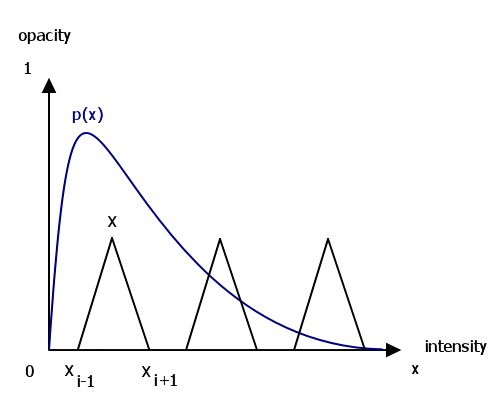
\includegraphics[width=0.6\textwidth]{drawing_distribution.png}
%  \caption{A transfer function with three components which correspond to three intensity intervals}
%  \label{fig:drawing_distribution}
%\end{figure}

%A typical class of 1D (intensity-based) transfer function is based on linear ramps between user-specified control points.

%Volume rendering is used to display a 2D image of a three-dimensional (3D) dataset. It can be seen as a projection of a 3D volumetric dataset into a two-dimensional (2D) image.
%In volume rendering, every volumetric element (voxel) must be mapped to opacity and a color.
%This is done with a transfer function, which can be a simple ramp, a piecewise linear function or an arbitrary table.
%Figure~\ref{fig:konig_mastering_2000} displays four typical shapes used in transfer function design.
%%All the four shapes can reveal structures in volume data sets.
%For volume data sets with complex structures, tent-like shapes are more effective in revealing isosurfaces of structures and seeing through inner structures. Otherwise, the ramp shape and other shapes can also reveal structures effectively.

\begin{table}
\centering
%\begin{minipage}{.5\textwidth}
\normalsize
\begin{tabular}{llll}
\hline
air & fat & soft tissue & bone (cancellous/dense)\\
\hline
-1000 & -100 to -50 & +100 to +300 & +700 to +3000\\
\hline
\end{tabular}
\caption{Hounsfield units of some typical substances \cite{feeman_mathematics_2009}}
\label{table:Hounsfield_unit}
%\end{minipage}
\end{table}

\begin{figure}
\centering

\begin{subfigure}{.24\textwidth}
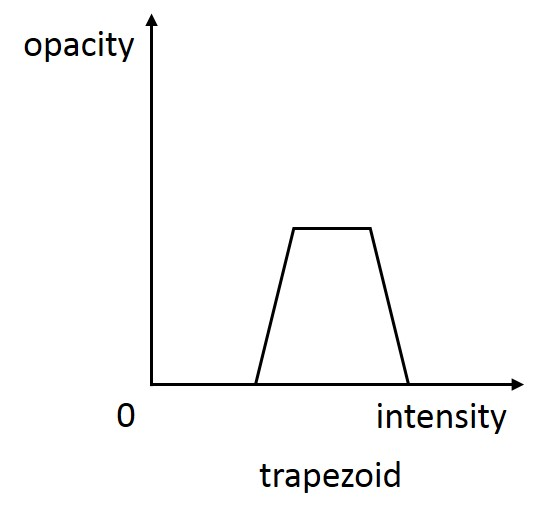
\includegraphics[width=1\textwidth]{konig_mastering_2000-zhou_automatic_2009_a.jpg}
\end{subfigure}
\begin{subfigure}{.24\textwidth}
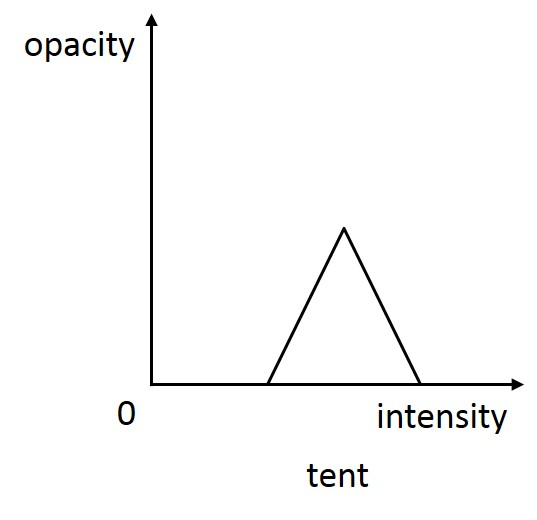
\includegraphics[width=1\textwidth]{konig_mastering_2000-zhou_automatic_2009_b.jpg}
\end{subfigure}
\begin{subfigure}{.24\textwidth}
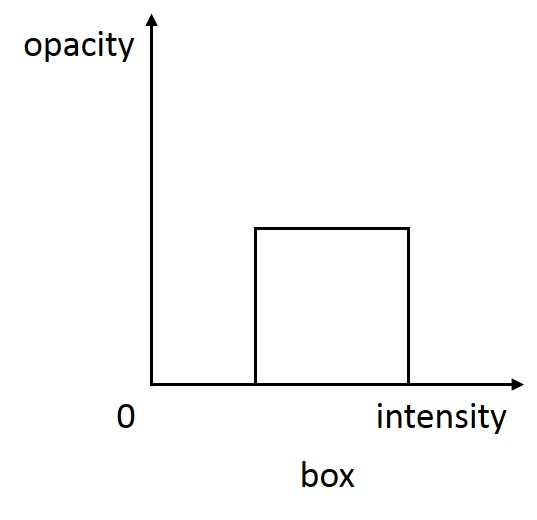
\includegraphics[width=1\textwidth]{konig_mastering_2000-zhou_automatic_2009_c.jpg}
\end{subfigure}
\begin{subfigure}{.24\textwidth}
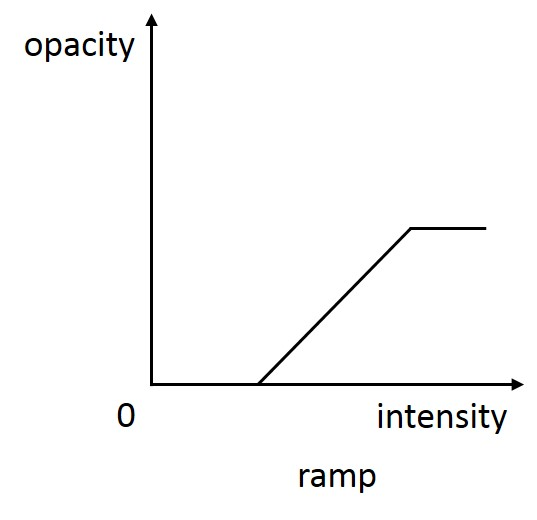
\includegraphics[width=1\textwidth]{konig_mastering_2000-zhou_automatic_2009_d.jpg}
\end{subfigure}
\caption{Typical transfer function shapes \cite{konig_mastering_2000}}
\label{fig:konig_mastering_2000}
\begin{subfigure}{.6\textwidth}
\centering
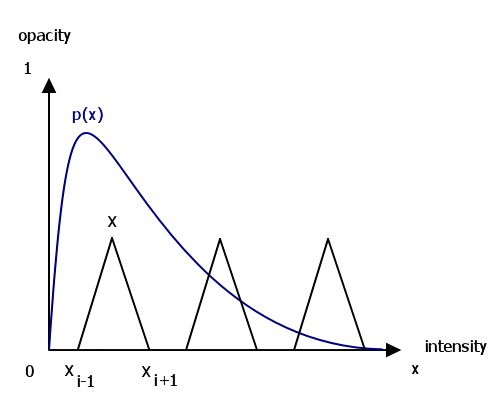
\includegraphics[width=1\textwidth]{drawing_distribution.png}
\end{subfigure}
\caption{A transfer function with tent-like shapes}
\label{fig:drawing_distribution}
\end{figure}

In the specification of a 1D (intensity-based) transfer function, the user essentially assigns a color and/or opacity to a certain point in the histogram of scalar values in the data set. In practice, the user would be presented with an interface that allows them to set up several control points which corresponds to a certain kind of material or structure. The user then defines a mapping from each control points to some visual property (e.g. color) resulting in voxels of the corresponding intensity to be rendered in that color.
Figure~\ref{fig:konig_mastering_2000} displays four typical shapes used in transfer function design.
%All the four shapes can reveal structures in volume data sets.
If a volume data set contains complex structures, tent-like shapes are desirable in revealing isosurfaces of structures and seeing through inner structures. Otherwise, the ramp shape and other shapes can also reveal structures effectively.% \cite{zhou_automatic_2009}

In order to design transfer functions effectively, it is commonly required that users have prior knowledge about which intensity ranges are relevant or which regions should be emphasized in the data. This is especially the case in medical visualization. For instance, in computed tomography (CT) data the intensity ranges are determined by the Hounsfield scale (Table~\ref{table:Hounsfield_unit}). The user may expect the constituent's intensity of CT data to follow the Hounsfield scale and thus set up control points accordingly.
%For instance, they might chose that bone should be mapped on to white and muscle to blue.
%However, small changes made to the opacity of control points may lead to dramatic changes in the rendered images.
%In many cases, minuscule modulation of opacity is required, but this kind of tiny adjustment of control points may be impossible to make accurately through mouse interaction due to limited accuracy of mouse movements.

%Another consideration is that voxels of a particular color can be more visually meaningful to the viewer than voxels of another color.
%An observation by Bordoloi and Shen \cite{bordoloi_view_2005} is that voxels of a particular color can be more visually meaningful to the viewer than voxels of another color.
%For instance, if there are two groups of voxels with different intensity in a scene, if the size of the first group of voxels is considerably less than the second one, then it is possible that the second group of voxels completely occludes the first one.
%Features inside other material are likely to be of far less voxels and are often occluded by the surrounding material.
%Additionally, Gestalt principles \cite{pessoa_finding_1998} suggest that the human mind would extrapolate the larger object (called ground) behind the smaller one (called figure). Thus the first group of voxels should have higher importance than the second one in order to be seen or distinguished.
Another consideration is that interior structures are likely to comprise far fewer voxels and are often occluded by the surrounding material.
Consider the transfer function in Figure~\ref{fig:drawing_distribution}. The user finds three intensity intervals of interest and then sets up three sets of control points in order to visualize these intensity intervals. The opacity of the three peak control points are assigned equally as they are equally important.
However, if the distribution of voxels follows $ p(x) $ (the blue curve), the voxels of the leftmost intensity intervals may completely occlude voxels of the other two intensity intervals in the resulting image.
The global optimization in our approach aims at reducing this kind of occlusion by modulating the opacity of the transfer function based on the distribution of scalar values of the volume data set.
%Figure~\ref{fig:multiple_nucleon} illustrates a transfer function which is more appropriate in this situation.

\subsection{Entropy of Volume Data}
In computer graphics, information-theoretic measures, such as entropy and mutual information, have been applied to solve multiple problems in areas such as view selection \cite{bordoloi_view_2005} 
%\cite{takahashi_feature-driven_2005}
\cite{bramon_information-theoretic_2013}, flow visualization \cite{xu_information-theoretic_2010}, multi-modal visualization \cite{haidacher_information-based_2008} \cite{bramon_information_2013} and transfer function design \cite{bruckner_isosurface_2010} \cite{ip_hierarchical_2012}.
Information theory provides a theoretic framework to measure the information content (or uncertainty) of a random variable represented as a distribution \cite{wang_information_2011}.
Consider a discrete random variable X which has a set of possible values $\{a_{0},a_{1},...,a_{n-1} \}$ with probabilities of occurrence $\{ p_{0},p_{1},...,p_{n-1} \}$, we can measure the uncertainty of the outcome with the entropy H(X), which is defined by
\[  H(X)=-\sum_{x \in X} p(x) \log p(x) \]
where the summation is over the corresponding alphabet and the convention $ 0\log 0=0 $ is taken% \cite{sbert_information_2011}
.
The term $ -\log p(x) $ represents the information content associated with the result x.
If the entire volume data set is treated as a random variable, $ I(a_{x})=-\log p(x) $ represents the information content of a voxel $ a_{x} $ with intensity x, and the entropy gives us the average amount of information of a volume data.
The probability p(x) is defined by
$ p(x)=\frac{n_{x}}{n} $, where $ n_{x} $ is the number of voxels with intensity x and n is the total number of voxels in the volume data.

%In Bordoloi and Shen \cite{bordoloi_view_2005}'s work for view selection of volume rendering, the entire volume data set is treated as a random variable.

%Bordoloi and Shen \cite{bordoloi_view_2005} and Takahashi et al. \cite{takahashi_feature-driven_2005} introduced the entropy to evaluate the quality of a viewpoint.

%In Bordoloi and Shen's work \cite{bordoloi_view_2005}, 

Bordoloi and Shen \cite{bordoloi_view_2005} described a noteworthiness factor to denote the significance of the voxel to the visualization.
The noteworthiness should be high for the voxels which are desired to be seen, and vice versa. The noteworthiness of voxel $ j $ is defined as
$ W_{j}=\alpha_{j}I_{j}=-\alpha_{j}logf_{j} $
, where $ \alpha_{j} $ is the opacity of voxel $ j $ looked up from the transfer function, $ I_{j} $ is the information carried by voxel $ j $, which can be derived from the frequency of its histogram bin $ f_{j} $. -log $ f_{j} $ represents the amount of information associated with voxel $ j $.

\section{Method}
In this section, we present a transfer function refinement approach for modulating the opacity associated with the control points in a transfer function and combine it with user interaction to specify priority areas or intensity values of importance in the resulting image. In previous work \cite{luo_information-guided_2014} we proposed a weighting of control points of transfer functions and an optimization method to minimize the energy function based on this weighting. However, this approach was limited to refining transfer functions with tent-like shapes and processing static volume data sets. 
In this paper we extend this approach with a more general distribution of weightings and energy function, so that it can handle any form of one-dimensional transfer function based on control points. In addition, an interaction widget (as in Figure~\ref{fig:CT-Knee_hue_selection}) is introduced to allow users to explore the data sets by emphasizing certain intensity values and see the optimized output immediately.
%In order to help the user explore the data sets, we combine the automatic optimization process with intuitive user interaction to specify priority areas or intensity values of importance in the resulting image.

In our approach, the user has control of the transfer functions by setting up control points as input for the optimization or tweaking the resulting transfer functions after the optimization. For example, the user can leave out less relevant data ranges by not covering the data ranges with shapes formed by control points (as in Figure~\ref{fig:konig_mastering_2000}). In the case of refining existing transfer functions, users also have the flexibility to refine the input transfer functions partially and keep certain control points constant during the optimization.

\subsection{Weighting of Transfer Function Components}
The goal of our transfer function refinement approach is to balance the opacity settings so that voxels of more significance contribute more and voxels of less significance contribute less to the resulting images.
%An assumption we made in this thesis (Section \ref{motivation}) is that the importance of voxels are associated with their information content. 
%In our approach, the intensity range of the transfer function are normalized to $ [0,1] $.
Given the intensity of the control points $ v_{1},v_{2},...,v_{n} $ of the transfer function $ t $ are $ x_{1},x_{2},...,x_{n} $ and the corresponding opacity are $ \alpha(x_{1}),\alpha(x_{2}),...,\alpha(x_{n}) $. The intensity range of the transfer function is normalized to $ [0,1] $.
For the convenience of discussion, two control points $ v_{0} $ and $ v_{n+1} $ are added to the lower bound and the upper bound respectively, and $ x_{0}=0 $, $ \alpha(x_{0})=0 $, $ x_{n+1}=1 $ and $ \alpha(x_{n+1})=0 $.

Similar to the noteworthiness factor by Bordoloi and Shen \cite{bordoloi_view_2005}, opacity and probability (derived from the intensity histogram) are also used in our weighting.
We define the significance factor of the intensity $ x $ as
\[
s(x)=-\alpha(x)p(x) \log p(x), x \in [0,1]
\]
In the significance factor $ s(x)$, $ p(x) $ is computed from the histogram of the data set, and $ \alpha(x) $ is the opacity function that we want to modulate.
The significance factor should be high for the voxels which are desired to be seen, and vice versa.
Then we define the weight of the $ i $-th edge (the segment between $ v_{i} $ and $ v_{i+1} $) as
\[
e(i)=\int_{x \in [x_{i}, x_{i+1}]} s(x) dx
\]
where $ i \in [0,n]$ and $ x \in [0,1] $.

Hence the energy function with distance factors for the intensity $ x_{0} $ of the transfer function can be defined as the variance of edge weights with the distance factors
\[
E=\sum_{i=0}^{n}(e(i)-\overline{e(i)})^{2}
\]
where $ \overline{e(i)} $ is the mean of edge weights, i.e.
\[
\overline{e(i)}= \frac{\sum_{i=0}^{n}e(i)}{n}
\]
%
%and define the significance factor of the $ i $-th control point as the sum of the weights of its two adjacent edges
%\[
%V(i)=E(i)+E(i-1), i \in [1,n]
%\]
%Then the average significance factor of all the control points is
%\[
%V_{mean}= \frac{\sum_{i=1}^{n}V(i)}{n}
%\]
%Hence the energy function of the transfer function $ t $ can be defined as the variance of the significance factors of control points
%\[
%F(t)=\sum_{i=1}^{n}(V(i)-V_{mean})^{2}
% \]

Consequently, minimizing the energy function is equivalent to flattening the curve of the edge weights.

\subsection{Optimizer}
\label{sec:optimizer}
Constraints are introduced in the search of the parameter space. Control points would only be moved vertically in the transfer function domain. In other words, only the opacity associated with control points would be changed. The intensity of control points remains the same. Also, those control points that are marked as constant would not be updated in the optimization process.
These constraints are based on our assumption that the intensity intervals associated with control points are the user's intensity intervals of interest. The user has explored the volume data and set up the transfer function according to his/her needs. Our algorithm aims to help the user reduce occlusion while preserving the user's knowledge or judgments of the data set.

A greedy strategy is employed in our algorithm to minimize the energy function. In each iteration, two operations are performed:
\begin{itemize}
\item Find the edge with the highest weight in the transfer function and reduce the opacity of the control point at its upper end (the vertex with a larger significance factor in the edge's two adjacent vertices).
\item Find the edge with the lowest weight in the transfer function and increase the opacity of the control point at its lower end (the vertex with a smaller significance factor in the edge's two adjacent vertices).
\end{itemize}
%reducing the opacity of the highest control point (with highest significance factor) and increasing the opacity of the lowest control point (with non-zero lowest significance factor).

In our implementation, the optimization ends when it reaches a user-specified iteration count.
The two step sizes in reducing opacity and increasing opacity can both be user-specified, or the first one is user-specified and the second one is computed based on the first one and the ratio of the significance factors of the two chosen control points. The ratio of the two step sizes affects the overall opacity of the resulting image, for instance, the image becomes more opaque or translucent.

\subsection{Distance Factors for Prioritizing Intensity Ranges}
\label{interaction_methods}
The above described optimizer is an approach to balance the global opacity and thus reduce occlusions in the rendered images. In other words, we de-emphasize the most prevalent voxels, which are considered to have a high probability of occluding the rest of the scene and in particular interior structures of the data.

Although global optimization can help deliver images with better overall visibility, small details may be under-enhanced in the global optimization and certain structures in the image may have to be further enhanced for specific purposes. For instance, in an anatomical data set, the global optimization may guarantee that all structures of materials such as skin, bone and flesh are all visible however if the task of the user is specifically to study skin, this may be counter-productive. Thus, it is clear that a flexible method guided by user interactions is necessary to achieve various visualization goals. 

In this section, we describe two alternative methods for prioritizing specific intensity ranges in the volume data. The first approach allows the user to interactively select a specific intensity range target that they are interested in and a hue-based distance factor is used to emphasize different intensity ranges based on the target identified by the user. Secondly, we describe a region-based optimization to provide an intuitive method of interaction by choosing regions of interest in the image that are then enhanced in the final rendering.

\subsubsection{Distance Factors for User-Selected Intensity Values}
%In addition, our optimization approach can be applied to explore different intensity ranges in volume data sets.

%We introduce hue-based distance factors to prioritize the specific intensity ranges. 
%Assume each control point is assigned a unique color, we can get the difference of hue in HSV color space between a specific color and the color of a control point.

We introduce distance factors for intensity values to prioritize the specific intensity ranges.
In our implementation, the user can select an intensity value by clicking on a color palette, which uses the same color map in the transfer function.
Assume each control point is assigned a unique intensity value, we can get the difference between a specific intensity value and the intensity value of a control point.

Given the selected intensity $ x_{0} $, we define the distance factor of the $ i $-th control point $ x(i) $ as
\[  D_{h}(i)=|x_{0}-x(i)|, i \in [0,n+1] \]
Linear interpolation is used to obtain the distance factor $ d_{h}(x) $ for the intensity $ x \in [x_{i},x_{i+1}) $

\[ d_{h}(x)=D_{h}(i) + (D_{h}(i+1)-D_{h}(i))\frac{x-x_{i}}{x_{i+1}-x{i}} \]

Therefore, we define the weight of the $ i $-th edge (the segment between $ v_{i} $ and $ v_{i+1} $) with the distance factors as
\[
e_{h}(i)=\int_{x \in [x_{i}, x_{i+1}]} d_{h}(x)s(x) dx
\]
where $ s(x)=-\alpha(x)p(x) \log p(x), x \in [0,1], i \in [0,n]$.

Hence, the energy function with distance factors for the intensity $ x_{0} $ of the transfer function can be defined as the variance of edge weights with the distance factors
\[
E_{h}=\sum_{i=0}^{n}(e_{h}(i)-\overline{e_{h}(i)})^{2}
\]
where $ \overline{e_{h}(i)} $ is the mean of edge weights $e_{h}(i)$.
%, i.e.
%\[
%\overline{e_{h}(i)}= \frac{\sum_{i=0}^{n}e_{h}(i)}{n}
%\]

To use the energy function $ E_{h} $ described in this section, we simply need to replace the original energy function with $ E_{h} $ in the previously described optimization algorithm.

%In our approach, the sum of the squared distances $ D_{s} $ between each pixel in the region $ R $ and the $ i $-th control point is used to measure the difference between the region and the control point.
%\[ D_{s}(R,i)=\sum_{r \in R}d(r,c(i))^{2} , i \in [1,n] \]
%We define the difference factor between the region $ R $ and the $ i $-th control point as
%\[ W(R,i)=\frac{D_{s}(R,i)}{\sum_{i=1}^{n}D_{s}(R,i)}, i \in [1,n] \]

%Hence, the distance factor of the $ i $-th control point is
%\[ V_{h}(i)=d_{h}V(i), i \in [1,n] \]
%To use this distance factor with the optimization algorithm described above, we simply need to replace $ V(i) $ with $ V_{h}(i) $ and compute the mean of significance factors accordingly in the energy function.

\subsubsection{Distance Factors for User-Selected Regions}
%In our approach, user manipulations are supported in the transfer function domain. Users can specify opacity values for control points in the transfer function to indicate their importance.
%This user-specified weighting would be taken into account in the optimization process.
In addition to selecting a specific intensity value, the distance factors can also be calculated using a region selected by the user. This region-based selection provides an intuitive method for the user to prioritize specific intensity ranges by selecting a region with the colors of interest in the resulting image.

We introduce region-based distance factors to prioritize the user's region of interest.
%The difference factors indicate the dissimilarity in color between a selected region in the final image and each control point.
%The weighting represents how much the control point contributes to the selected region.
Assume each control point is assigned a unique color, we can get the difference between the color of a pixel in the region (which is selected in image space) and the color of a control point (HSV color space is used in our implementation).

Given the color of the $ i $-th control point is $ c(i) $, the distance between the color of a pixel $ r $ in the region $ R $ and the color of the $ i $-th control point is denoted by $ d(r,c(i)) $. In our approach, the sum of the distances $ D $ between each pixel in the region $ R $ and the $ i $-th control point is used to measure the difference between the region and the control point.
\[ D(R,i)=\sum_{r \in R}d(r,c(i)) , i \in [0,n+1] \]
%We define the distance factor between the region $ R $ and the $ i $-th control point as
Given the selected region $ R $, we define the distance factor of the $ i $-th control point as 
\[ W_{R}(i)=\frac{D(R,i)}{\sum_{i=1}^{n}D(R,i)}, i \in [0,n+1] \]
Linear interpolation is used to obtain the distance factor $ w_{R}(x) $ for the intensity $ x \in [x_{i},x_{i+1}) $

\[ w_{R}(x)=W_{R}(i) + (W_{R}(i+1)-W_{R}(i))\frac{x-x_{i}}{x_{i+1}-x{i}} \]

Therefore, we define the weight of the $ i $-th edge (the segment between $ v_{i} $ and $ v_{i+1} $) with the distance factors as
\[
e_{R}(i)=\int_{x \in [x_{i}, x_{i+1}]} w_{R}(x)s(x) dx
\]
where $ s(x)=-\alpha(x)p(x) \log p(x), x \in [0,1], i \in [0,n]$.

Hence, the energy function with distance factors for the region $ R $ of the transfer function can be defined as the variance of edge weights with the distance factors
\[
E_{R}=\sum_{i=0}^{n}(e_{R}(i)-\overline{e_{R}(i)})^{2}
\]
where $ \overline{e_{R}(i)} $ is the mean of edge weights $e_{R}(i)$.
%, i.e.
%\[
%\overline{e_{R}(i)}= \frac{\sum_{i=0}^{n}e_{R}(i)}{n}
%\]

%To use the energy function $ E_{R} $ described in this section, we simply need to replace the original energy function with $ E_{R} $ in the previously described optimization algorithm.

Similarly, in order to use the energy function $ E_{R} $, we need to replace the original energy function with $ E_{R} $ in the previously described optimization algorithm.

%Consequently, the modified significance factor (biased towards the region $ R $) of the $ i $-th control point is
%\[ V_{R}(i)=W_{R}(i)V(i), i \in [1,n] \]
%To use this significance factor with the optimization algorithm described above, we simply need to replace $ V(i) $ with $ V_{R}(i) $ and compute the mean of significance factors accordingly in the energy function.

The distance factors described in this section measure the dissimilarity between a selected region and a control point. Therefore, the distance factor would be small if the region has an overall color similar to the color of the control point.
Since we are minimizing the energy function, which is the variance of the edge weights, reducing the distance factors of those control points, which are related to the selected region, will result in their opacity values being increased. As a result, the features (in this case, the intensity intervals) in the selected regions will be enhanced and other features will be de-emphasized in the rendered image.
%The distances in $ D_{s}(R,i) $ are squared, therefore, it results in a weighting which is more biased towards the selected region, compared to the weighting based on non-squared distances.
%It thus leads to further enhanced features with further weaken context in the rendered images.
Since the distance is measured in the color space, the choice of colors for the control points affects the measured distance and thus affects the weighting function.
%For the purpose of generating satisfactory weighting, control points are better to be assigned colors which are dispersed in the color space.

%In addition, other color spaces could be adopted in this approach. The CIE L*u*v* (abbreviated CIELUV) color space, which is a perceptually uniform representation of the color volume, is a potential alternative in terms of measuring difference. Because the CIE L*u*v* color space is perceptually uniform, it has the characteristic that equally distances in the color space correspond to equal perceptual differences, at least for reasonable small distances \cite{ebert_designing_2002}.

\subsection{Adaptive Transfer Functions for Time-Varying Data Sets}
In time-varying data sets, the data value ranges and distributions change among time-steps. A single global transfer function may not be able to adequately catch the details of the data set.
Therefore, we exploit the transfer function optimizer (as discussed in Section~\ref{sec:optimizer}) to locally refine the transfer function for each time-step in the data set.
In this case, the user specifies a transfer function for a single time-step of the time-varying data set and using either of the two interaction methods (as discussed in Section~\ref{interaction_methods}) to specify priority intensity ranges.
The transfer function designed for this time-step is taken as an input transfer function and optimized again based on the histogram of the next time-step. Subsequently, the output of next time-step is taken as input of the time-step after it and so forth.

\section{Results and Discussions}
In this section, we present some results to demonstrate the effectiveness of our approach on the CT-knee (379 $ \times $ 229 $ \times $ 305) and VisMale head (128 $ \times $ 256 $ \times $ 256) data sets \cite{website:Roettger_volume_2013} and a time-varying data set of a simulated turbulent vortex flow (128 $\times$ 128 $\times$ 128, 100 time-steps) \cite{ma_high_2000}.
%and four volumes of a horse embryo data set, which are the horse embryo at 35, 37, 39 and 42 days.
Results were generated in our volume rendering system (Figure~\ref{fig:volume_visualizer}) on a computer equipped with an Intel Core i5-2410M CPU, 8GB of RAM and an NVIDIA GeForce GT 540M graphics card.
%Tests were performed on a computer equipped with an Intel Core i5-2410M CPU, 8GB of RAM and a NVIDIA GeForce GT 540M graphics card.

\begin{figure}
    \centering
	\begin{minipage}{.9\textwidth}
        \centering
        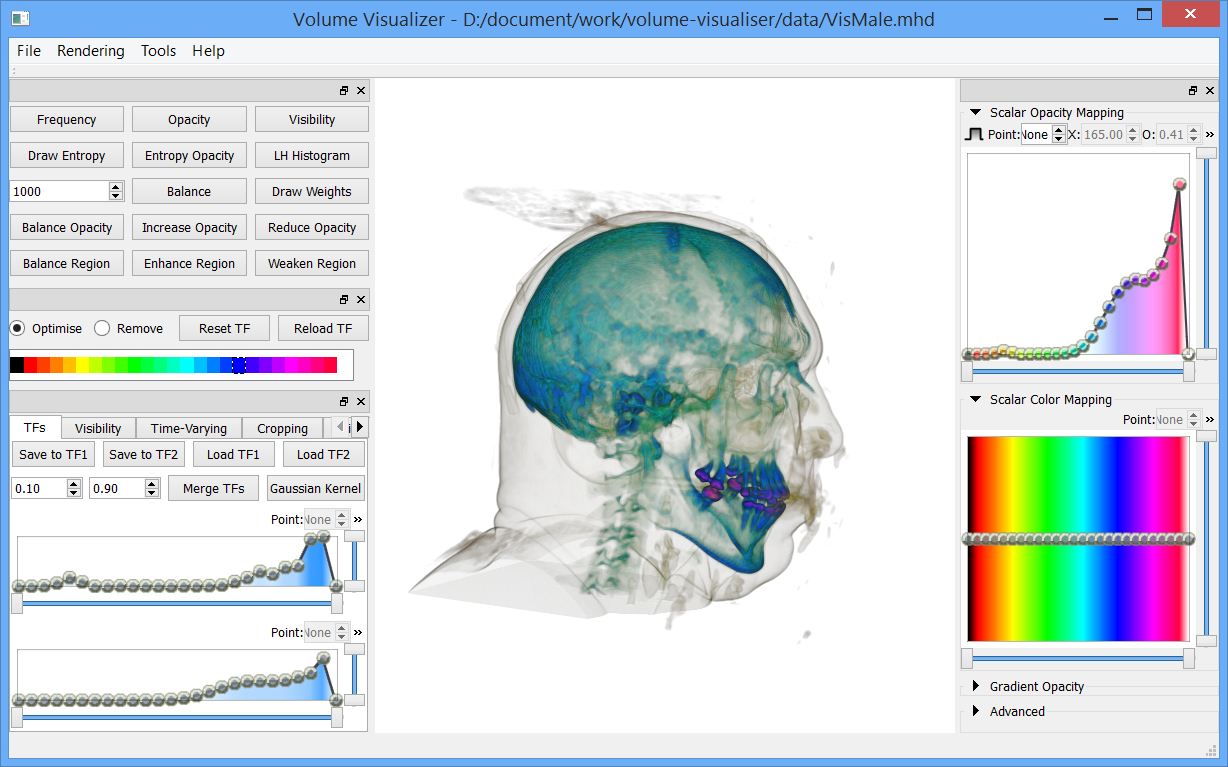
\includegraphics[width=\textwidth]{volume_visualizer.png}
        \caption{A screen shot of our volume rendering system}
        \label{fig:volume_visualizer}
	\end{minipage}
\end{figure}

Automatically generated transfer functions with ramps and tent-like shapes are provided as initial input to the optimizer. Figure~\ref{fig:tf_CT-Knee_spectrum_16_ramp} displays a continuous transfer function. The ramps are formed by a series of control points with corresponding colors from the color map.
Figure~\ref{fig:tf_CT-Knee_spectrum_6} displays a transfer function with several evenly distributed tent-like shapes. Each tent-like shape consists of a peak control point and two bottom control points. The peak control points are movable while the bottom control points are marked as constant to maintain the tent-like shapes.

Note that the transfer functions consisting of equidistant and equal height tent-like shapes (as in Figure~\ref{fig:tf_CT-Knee_spectrum_6}) are just provided as naive examples of user designed transfer functions and used as input to the optimizer. In practice, users would design transfer functions (which consist of ramps, tent-like or other shapes) according to the characteristic of the data sets and the intensity ranges that they are interested in.

%Automatically generated transfer functions with evenly distributed control points are used as the input of the optimization. Two kinds of transfer functions are used in our experiments. One is transfer functions with tent-like shapes (as in Figure~\ref{fig:tf_CT-Knee_spectrum_6} and Figure~\ref{fig:tf_CT-Knee_spectrum_6_balance_1000}), which consist of a number of control point groups (3 control points of the same color) and gaps among the groups. The other is continuous transfer functions (as in Figure~\ref{fig:tf_CT-Knee_spectrum_16_ramp} and Figure~\ref{fig:tf_CT-Knee_spectrum_16_ramp_balance}), which are continuous ramps with control points of different colors.
%Two kinds of transfer functions are used in our experiments.
%One is transfer functions with tent-like shapes (as in Figure~\ref{fig:tf_CT-Knee_spectrum_6} and Figure~\ref{fig:tf_CT-Knee_spectrum_6_balance_1000}), which consist of a number of control point groups (3 control points of the same color) and gaps among the groups. 
%The other is continuous transfer functions (as in Figure~\ref{fig:tf_CT-Knee_spectrum_16_ramp} and Figure~\ref{fig:tf_CT-Knee_spectrum_16_ramp_balance}), which are continuous ramps with control points of different colors.

The initial opacity values of control points will affect the overall opacity level of the resulting image after optimization. Because there are omitted intensity ranges (the gaps) in transfer functions with tent-like shapes, the initial opacity values should be higher in transfer functions with tent-like shapes than in continuous transfer functions.
In transfer functions with tent-like shapes (as discussed in Section~\ref{sec:background}), the opacity of the top control points are set to $ 1/2 $ and the opacity of the bottom control points are set to 0. The bottom control points are fixed to 0 in order to keep the tent-like shapes in the transfer functions. By contrast, all control points in continuous transfer functions are movable vertically except that control points $ v_{0} $ and $ v_{n+1} $ are fixed and serve as the boundary. The opacity of control points are set to $ 1/6 $ in continuous transfer functions.
The color maps used in the transfer functions in our system are evenly sampled from a spectrum (with hue from $ 0^\circ $ to $ 360^\circ $ in HSV color space).
%In the transfer functions, every three adjacent control points with the same color are considered a control point group corresponding to an intensity range.
In the optimization, the two step sizes for reducing opacity and increasing are both set to $ 1/256 $.
%The results below are rendered with Voreen \cite{meyer-spradow_voreen:_2009} after transfer function optimization using our approach.

\subsection{Automatic Transfer Function Refinement}
%\emph{Global Optimisation Results:}
Firstly, we demonstrate the global optimization with continuous transfer functions.
In Figure~\ref{fig:tf_CT-Knee_spectrum_16_ramp}, the CT-Knee data set is rendered with a naive transfer function consisting of 6 tent-like shapes of various colors with equal opacity. Figure~\ref{fig:tf_CT-Knee_spectrum_16_ramp_balance} shows the resulting image rendered with the optimized transfer function.
We tested this specific example as joints are popular regions of interest in medical visualization.
% and a number of researchers have extended volume rendering techniques to examine joints of human body \cite{borland_volumetric_2006}. 
The knee in particular is a commonly studied joint.
In Figure~\ref{fig:tf_CT-Knee_spectrum_16_ramp}, only parts of the skeleton are visible. The rest is occluded by the surrounding material (such as the skin and muscles).
%The knee joint is completely occluded by the surrounding tissues.
After optimization (Figure~\ref{fig:tf_CT-Knee_spectrum_16_ramp_balance}), the surrounding tissues become translucent, hence the skeleton is exposed and the knee joint is visible, while the overall context is preserved. We argue that in the absence of any previous assumptions on what the user is looking for, the global optimization provides a more balanced initial view before deeper exploration of the data.

Although the continuous transfer function is useful in automatic transfer function generation, in typical volume visualization programs, users often prefer much more simplified transfer functions, e.g. a few control points such as in transfer functions with tent-like shapes. Figure~\ref{fig:tf_CT-Knee_spectrum_6} is the CT-Knee data set rendered with the transfer function. We show in Figure~\ref{fig:tf_CT-Knee_spectrum_6_balance_1000} that our optimization can also benefit such simpler transfer functions.

In practice we observed that the energy function usually converges to a small but non-zero value. As the number of control points increases, it takes more iterations for the optimization to achieve a stable state - a number of tent-like shapes ranging from 4 to 16 was found to be the most effective.
Our approach is relatively lightweight, e.g. we observed that the optimization finished within one second on the CT-Knee and VisMale data sets with transfer functions consisting of 24 control points and maximum iteration count of 1000.

\begin{figure}
\centering

\begin{subfigure}{0.33\textwidth}
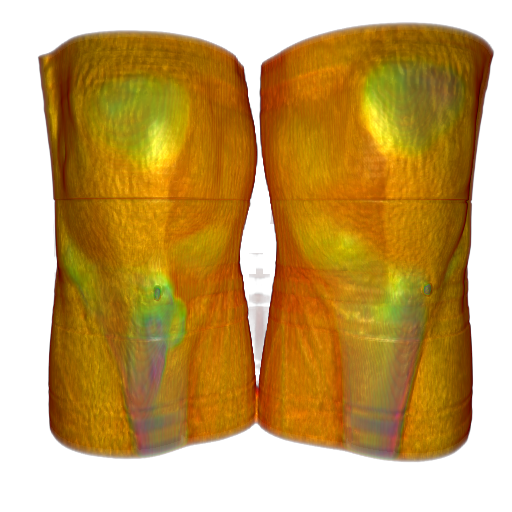
\includegraphics[width=\textwidth]{CT-Knee_spectrum_16_ramp.png}
\caption{~}
\end{subfigure}~
\begin{subfigure}{0.33\textwidth}
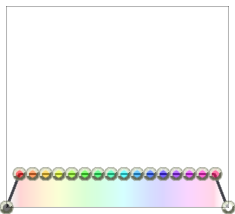
\includegraphics[width=\textwidth]{tf_CT-Knee_spectrum_16_ramp_.png}
\caption{~}
\label{fig:tf_CT-Knee_spectrum_16_ramp_}
\end{subfigure}~
\begin{subfigure}{0.33\textwidth}
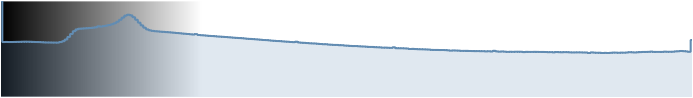
\includegraphics[width=1\textwidth,height=0.5\textwidth]{CT-Knee_histogram.png}
\caption{~}
\label{fig:CT-Knee_histogram}
\end{subfigure}
\caption{Before optimization: CT-Knee with a continuous transfer 
function (a) Preliminary view of data set (b) A continuous transfer 
function with a ramp (c) Histogram of the data set}
\label{fig:tf_CT-Knee_spectrum_16_ramp}

\begin{subfigure}{0.33\textwidth}
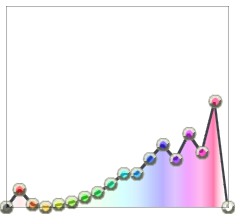
\includegraphics[width=\textwidth]{tf_CT-Knee_spectrum_16_ramp_balance_.png}
\caption{~}
\end{subfigure}
\begin{subfigure}{0.33\textwidth}
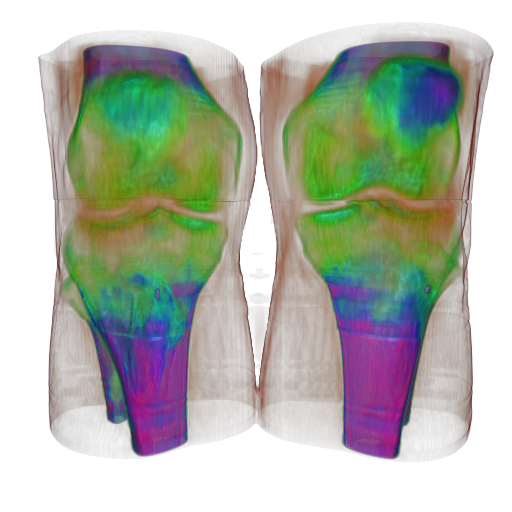
\includegraphics[width=\textwidth]{CT-Knee_spectrum_16_ramp_balance.png}    
\caption{~}
\end{subfigure}
\caption{The transfer function from Figure~\ref{fig:tf_CT-Knee_spectrum_16_ramp} after optimization: (a) Optimized transfer function) (b) Optimized output}
\label{fig:tf_CT-Knee_spectrum_16_ramp_balance}

\end{figure}

\begin{figure}
\centering

\begin{subfigure}{0.33\textwidth}
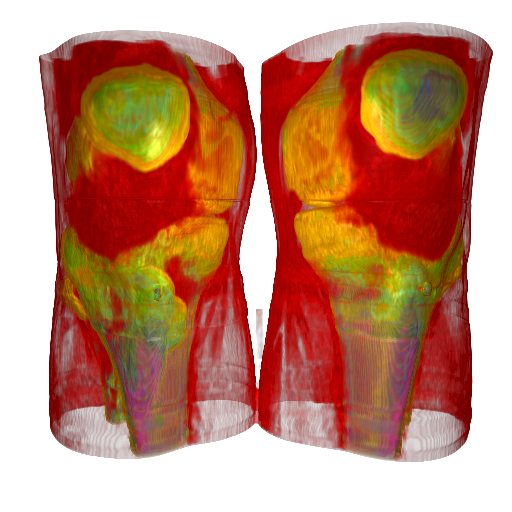
\includegraphics[width=\textwidth]{CT-Knee_spectrum_6_bump.png}
\caption{~}
\end{subfigure}
\begin{subfigure}{0.33\textwidth}
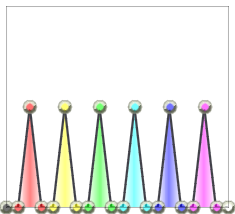
\includegraphics[width=\textwidth]{tf_CT-Knee_spectrum_6_bump_.png}
\caption{~}
\label{fig:tf_CT-Knee_spectrum_6_bump_}
\end{subfigure}
\caption{Before optimization: CT-Knee rendered with a transfer function consisting 
of tent-like shapes (a) Preliminary view of data set (b) A transfer function with 6 tent-like shapes}
\label{fig:tf_CT-Knee_spectrum_6}

\begin{subfigure}{0.33\textwidth}
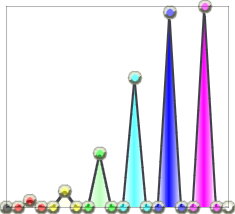
\includegraphics[width=\textwidth]{tf_CT-Knee_spectrum_6_bump_balance_.png}
\caption{~}
\end{subfigure}
\begin{subfigure}{0.33\textwidth}
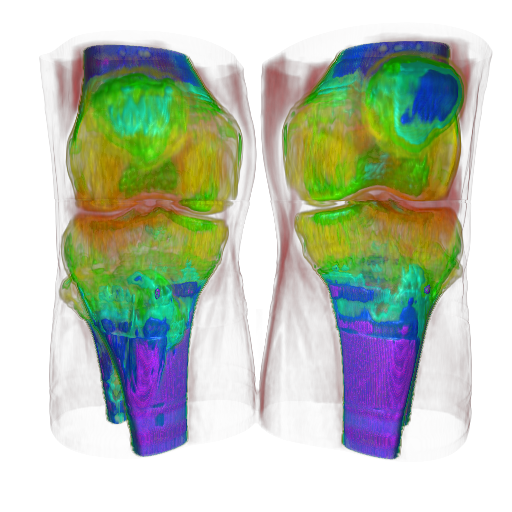
\includegraphics[width=\textwidth]{CT-Knee_spectrum_6_bump_balance.png}
\caption{~}
\end{subfigure}
\caption{The transfer function from Figure~\ref{fig:tf_CT-Knee_spectrum_6} after optimization: (a) Optimized transfer function (b) Optimized output}
\label{fig:tf_CT-Knee_spectrum_6_balance_1000}
\end{figure}

%\paragraph{Distance Factors}
\subsection{Transfer Function Refinement with User-Selected Intensity Values}
%optimising the transfer function to *improve* the exploration of volume data
%In this paragraph, we discuss the results of optimisation with distance factors for user-selected intensity values.
Figure~\ref{fig:CT-Knee_series} shows three images of a CT-Knee data set while different colors are selected for optimization. Since the colors of the transfer function are generated in HSV color space by varying the hue component, the difference of intensity values are mapped to the difference of hue in HSV color space. By clicking on the color palette (Figure~\ref{fig:CT-Knee_hue_selection}), the transfer function is instantly optimized for the corresponding intensity values.

\begin{figure}
    \centering	
	
	\begin{subfigure}{1\textwidth}
		\centering
		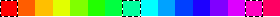
\includegraphics[width=\textwidth]{CT-Knee_hue_selection_2.png} 
	\end{subfigure}
	
	\begin{subfigure}{.3\textwidth}
	        \centering
	        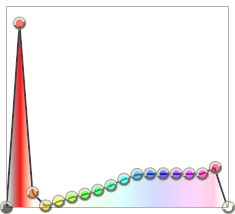
\includegraphics[width=\textwidth]{tf_CT-Knee_hue_00.png}
%	        \caption{}
	        \label{fig:tf_CT-Knee_hue_00.png}
	\end{subfigure}~
	\begin{subfigure}{.3\textwidth}
	        \centering
	        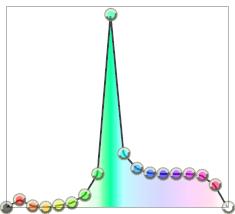
\includegraphics[width=\textwidth]{tf_CT-Knee_hue_07.png}
%	        \caption{}
	        \label{fig:tf_CT-Knee_hue_07.png}
	\end{subfigure}~
	\begin{subfigure}{.3\textwidth}
	        \centering
	        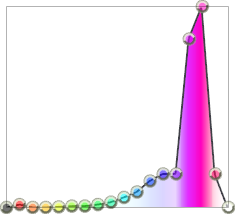
\includegraphics[width=\textwidth]{tf_CT-Knee_hue_14.png}
%	        \caption{}
	        \label{fig:tf_CT-Knee_hue_14.png}
	\end{subfigure}	
	
	\caption{The 3 chosen colors (corresponding to different intensity values) and the transfer functions after optimization for each intensity value. The same transfer function as shown in Figure~\ref{fig:tf_CT-Knee_spectrum_16_ramp} is used as input to the optimizer. Note how the transfer functions are enhanced for the specific intensity ranges as compared to the result of global optimization in Figure~\ref{fig:tf_CT-Knee_spectrum_16_ramp_balance}.}
	\label{fig:CT-Knee_hue_selection}    

	\begin{subfigure}{.33\textwidth}
        \centering
        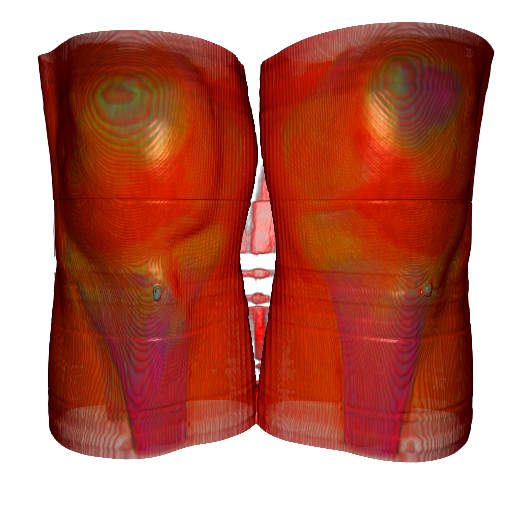
\includegraphics[width=\textwidth]{CT-Knee_hue_00.png}
        \caption{}
        \label{fig:CT-Knee_hue_00.png}
	\end{subfigure}~
	\begin{subfigure}{.33\textwidth}
        \centering
        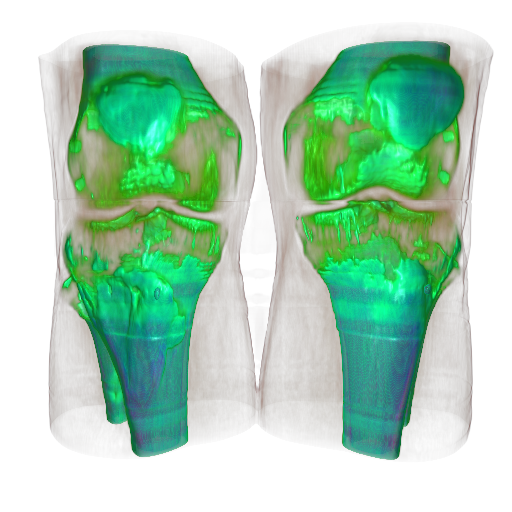
\includegraphics[width=\textwidth]{CT-Knee_hue_07.png}
        \caption{}
        \label{fig:CT-Knee_hue_07.png}
	\end{subfigure}~
	\begin{subfigure}{.33\textwidth}
	        \centering
	        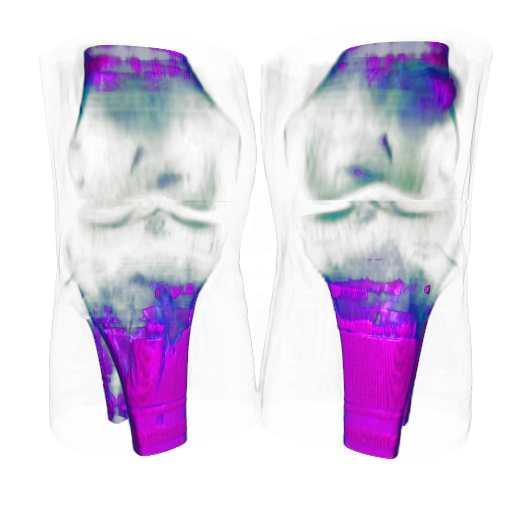
\includegraphics[width=\textwidth]{CT-Knee_hue_14.png}
	        \caption{}
	        \label{fig:CT-Knee_hue_14.png}
	\end{subfigure}
	\caption{The CT-Knee data with transfer functions optimized for the 3 colors in Figure~\ref{fig:CT-Knee_hue_selection}. (a) The materials with intensity values mapped to red are enhanced. Similarly, the materials in green and magenta are enhanced respectively in (b) and (c).}
	\label{fig:CT-Knee_series}	
\end{figure}

\subsection{Transfer Function Refinement with User-Selected Regions}
%\emph{Region-based optimisation}
Figure~\ref{fig:VisMale_spectrum_4_} shows the VisMale data set with a generated transfer function of 4 tent-like shapes. Figure~\ref{fig:VisMale_histogram} shows the intensity histogram of the data set.
%Figure~\ref{fig:VisMale_spectrum_4_balance_1000_} shows the image after optimization.
After the optimization (Figure~\ref{fig:VisMale_spectrum_4_balance_1000_}), the outside of the head is less opaque so the inner structures are revealed to the user. However, the intermediate material (i.e. the skull) also becomes less clear. If the goal is to make the skull more visible, the user could select a region consisting of parts of the skull to generate a weighting and perform further optimization of the transfer function. If the material of interest is occluded by surrounding materials, the user could use an axis-aligned clipping plane in order to accurately select voxels of the skull whilst minimizing the accidental tagging of the surrounding material (Figure~\ref{fig:VisMale_spectrum_4_clipplane_selection}).
%In this step, a clipping plane is used in order to allow the user to more accurately select voxels of the skull whilst minimizing the accidental tagging of the surrounding material.
As shown in Figure~\ref{fig:VisMale_spectrum_4_clipplane_region_1000}, the skull becomes more clear after the region-based optimization.

%A transfer function is manually specified (Figure~\ref{fig:multiple_CT-Knee}) to reveal parts of the bones. The global optimization is performed and more parts of the bones are revealed (Figure~\ref{fig:multiple_CT-Knee_balance}). However, the knee joint is still partial occluded. Then we selected a region of the bones and optimize the transfer function based on the weighting generated for this region. The knee joint is clearly exposed in the resulting images (Figure~\ref{fig:multiple_CT-Knee_region_distance}).
%
%Then we compare the results rendered with two different weighting generated for two selected regions. Figure~\ref{fig:multiple_VisMale7} is a transfer function with even distributed components. Figure~\ref{fig:multiple_VisMale7_balance} shows the result of global optimization. Figure~\ref{fig:multiple_VisMale7_selection} and Figure~\ref{fig:multiple_VisMale7_selection2} show the results of optimization based on two selected regions respectively. From Figure~\ref{fig:VisMale7_region_selection} and Figure~\ref{fig:VisMale7_region_selection} we can see how the two different weighting affects the rendering results.

\begin{figure}
        \centering
	\begin{subfigure}{.33\textwidth}
    \centering
    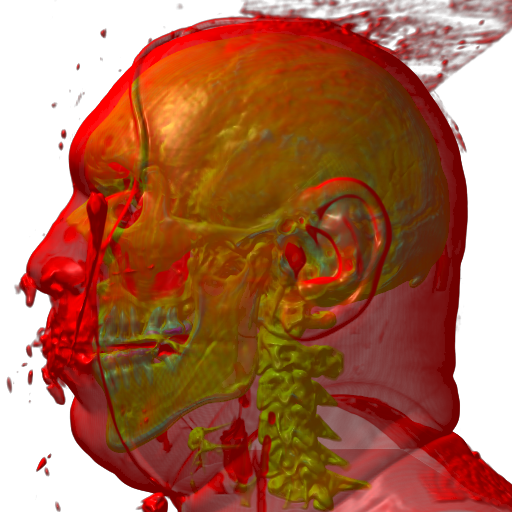
\includegraphics[width=\textwidth]{VisMale_spectrum_4.png}
    \caption{~}
    \label{fig:VisMale_spectrum_4_}
	\end{subfigure}~
	\begin{subfigure}{.33\textwidth}
    \centering
    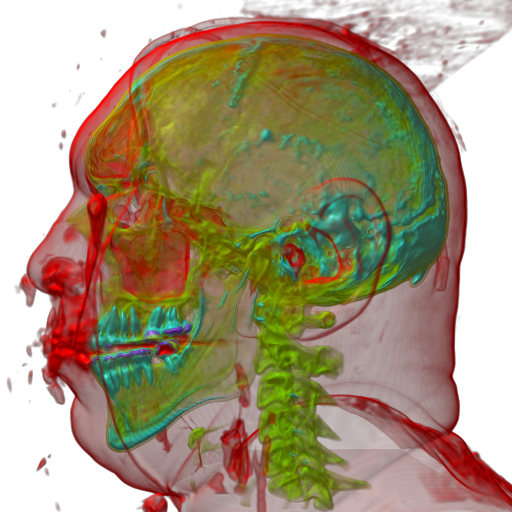
\includegraphics[width=\textwidth]{VisMale_spectrum_4_balance_1000.png}
    \caption{~}
    \label{fig:VisMale_spectrum_4_balance_1000_}
	\end{subfigure}~
	\begin{subfigure}{.33\textwidth}
	\centering
	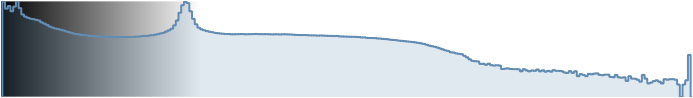
\includegraphics[width=1\textwidth,height=0.5\textwidth]{VisMale_histogram.png}
	\caption{~}
	\label{fig:VisMale_histogram}
	\end{subfigure}
	\begin{subfigure}{.33\textwidth}
	\centering
	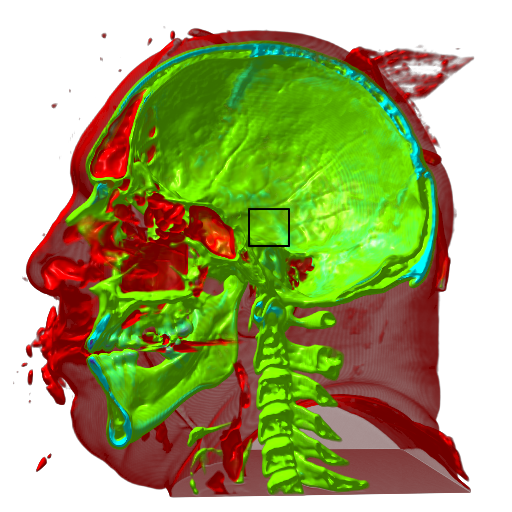
\includegraphics[width=\textwidth]{VisMale_spectrum_4_clipplane_selection.png}
	\caption{~}
	\label{fig:VisMale_spectrum_4_clipplane_selection}
	\end{subfigure}~
	\begin{subfigure}{.33\textwidth}
	\centering
	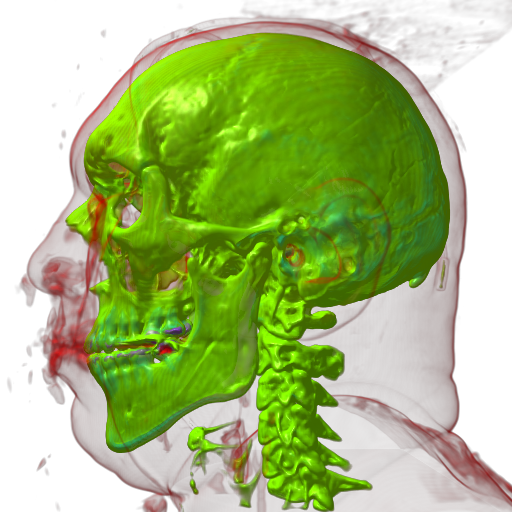
\includegraphics[width=\textwidth]{VisMale_spectrum_4_clipplane_region_1000.png}
	\caption{~}
	\label{fig:VisMale_spectrum_4_clipplane_region_1000}
	\end{subfigure}	
	\caption{(a) Preliminary view of the VisMale data set. (b) Optimized output. (c) Histogram of the data set. (d) The user selects a region on the skull under a clipping plane. (e) Optimized output: skull is enhanced and the outer layer is de-emphasized.}
	\label{fig:multiple_VisMale_spectrum_4_balance_1000}
\end{figure}

%\subsection{Combining Transfer Functions}
%Combine two transfer functions to obtain focus plus context effects.
%
%\begin{figure}
%    \centering	
%	\begin{minipage}{.45\textwidth}
%	        \centering
%	        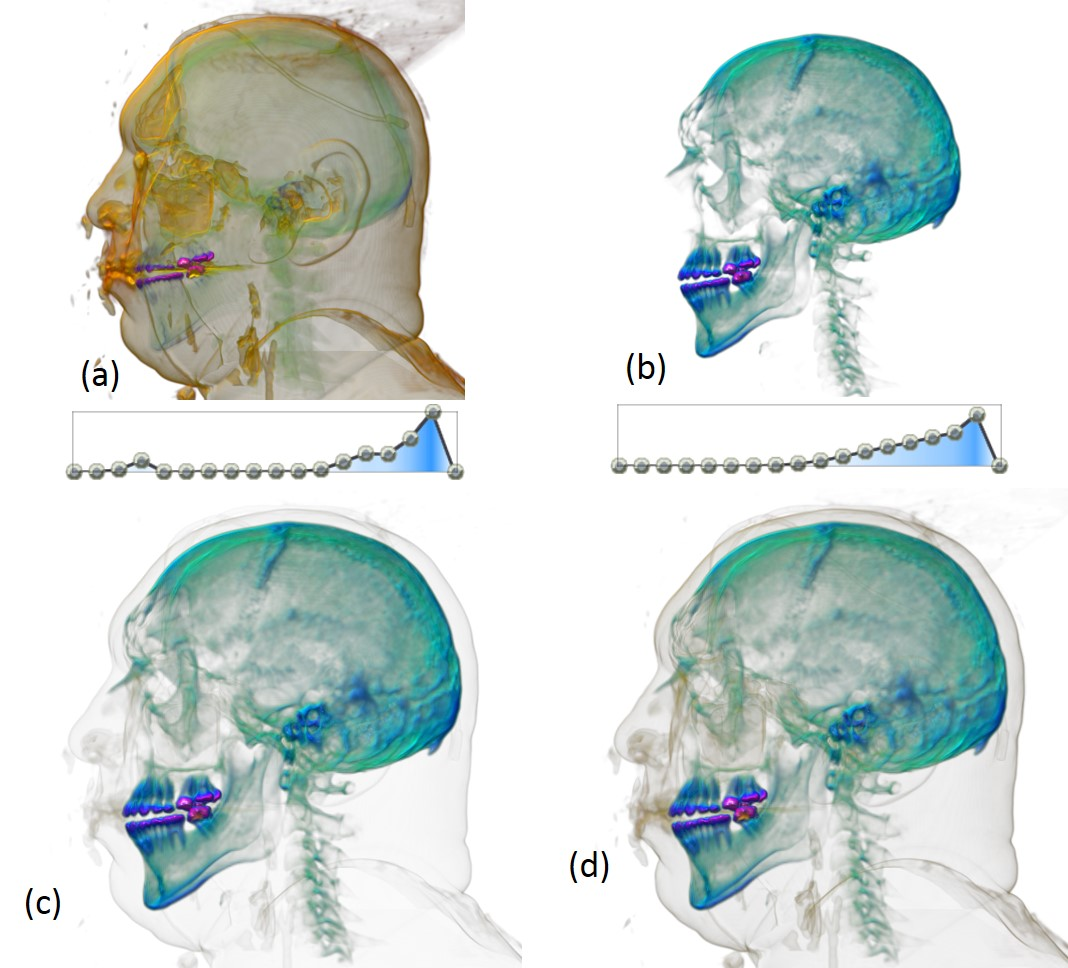
\includegraphics[width=\textwidth]{2_level.jpg}
%%	        \caption{Optimized for magenta}
%%	        \label{fig:2_level}
%	\end{minipage}
%	\caption{2 level}
%	\label{fig:2_level}	
%\end{figure}

\subsection{Adaptive Transfer Functions for Time-Varying Data Sets}
We demonstrate our approach on a turbulent vortex data set \cite{website:Ma_repository_2013}, which consists of 100 time-steps. Our optimizer adaptively propagates transfer functions for the time-varying data set. Specifically, the transfer function of the previous time-step is taken as input to generate the transfer function for the next time-step.
Therefore, the transfer functions are locally optimized for each time-step of the time-varying data set, but as the input transfer function comes from the immediate preceding time-step, the resulting transfer functions also exhibit reasonable temporal coherency assuming the data set is also coherent.
As the difference of intensity histograms among consecutive time-steps is hard to notice, only the images of the first time-step and a time-step in the middle of the data set are displayed here.
Figure~\ref{fig:vortex_series_time_00} shows three images of the vortex data set at time-step 0 while optimized for the three colors chosen in the color palette in Figure~\ref{fig:vortex_hue_selection}.
Figure~\ref{fig:vortex_series_time_50} displays the vortex data set at time-step 50 with the transfer functions optimized for the three chosen colors.
%Figure~\ref{vortex_time_00_histogram} and Figure~\ref{vortex_time_50_histogram} show the intensity histograms of the two time-steps discussed above.
%In the case that the user does not have much knowledge of a volume data set, our system renders the data set with different ranges being emphasized (see the transfer functions in Figure~\ref{fig:vortex_time_histogram}), in order to provide the user an automatic way to focus their exploration on different parts of the data set.
Figure~\ref{fig:vortex_time_histogram} shows the intensity histograms of the two time-steps discussed above and the corresponding optimized transfer functions for the colors selected in Figure~\ref{fig:vortex_hue_selection}.

\begin{figure}
\centering
	
\begin{subfigure}{1\textwidth}
\centering
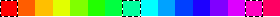
\includegraphics[width=\textwidth]{CT-Knee_hue_selection_2.png}
\end{subfigure}
\caption{The 3 chosen colors (corresponding to different intensity values) for optimization. Note how different parts of the data set are enhanced respectively in Figure~\ref{fig:vortex_series_time_00} and Figure~\ref{fig:vortex_series_time_50}.}
\label{fig:vortex_hue_selection}

\begin{subfigure}{.33\textwidth}
    \centering
    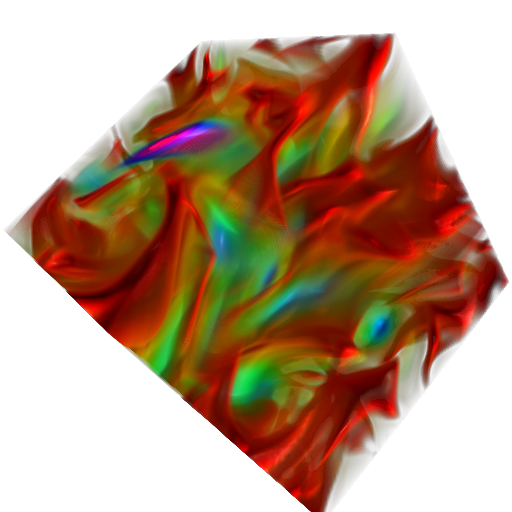
\includegraphics[width=\textwidth]{vortex_time_00_hue_00.png}
    \caption{~}
    \label{fig:vortex_time_00_hue_00}
\end{subfigure}~
\begin{subfigure}{.33\textwidth}
    \centering
    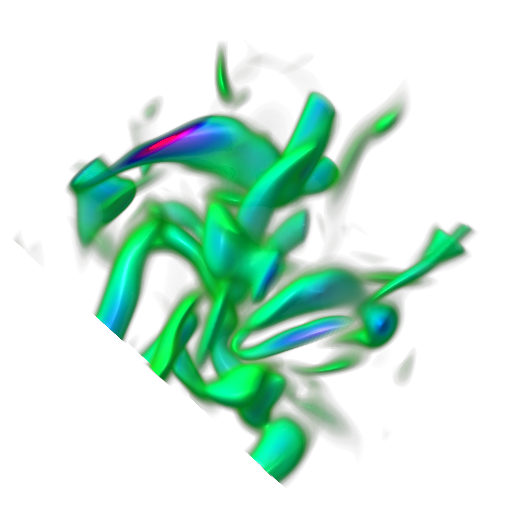
\includegraphics[width=\textwidth]{vortex_time_00_hue_07.png}
    \caption{~}
    \label{fig:vortex_time_00_hue_07}
\end{subfigure}~
\begin{subfigure}{.33\textwidth}
     \centering
     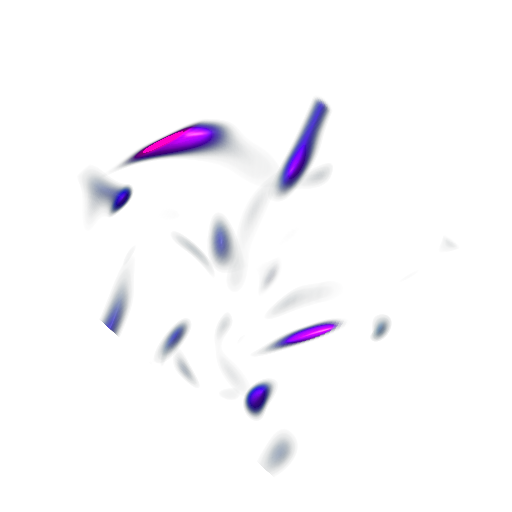
\includegraphics[width=\textwidth]{vortex_time_00_hue_14.png}
     \caption{~}
     \label{fig:vortex_time_00_hue_14}
\end{subfigure}
\caption{The vortex data at time-step 0. (a) The materials with intensity values mapped to red are enhanced. Similarly, the materials in green and magenta are enhanced respectively in (b) and (c).}
\label{fig:vortex_series_time_00}

\begin{subfigure}{.33\textwidth}
    \centering
    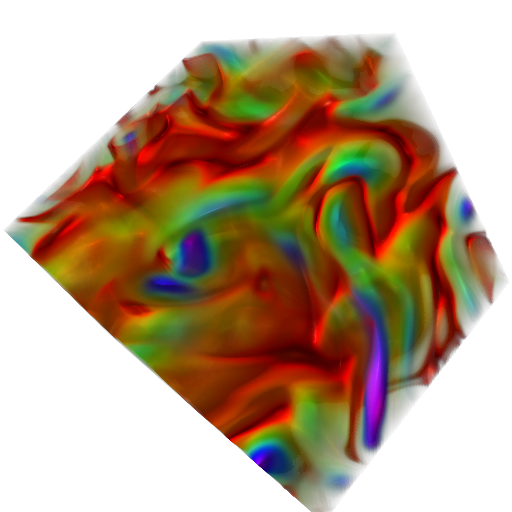
\includegraphics[width=\textwidth]{vortex_time_50_hue_00.png}
        \caption{~}
    \label{fig:vortex_time_50_hue_00}
\end{subfigure}~
\begin{subfigure}{.33\textwidth}
    \centering
    \includegraphics[width=\textwidth]{vortex_time_50_hue_07.png}
        \caption{~}
    \label{fig:vortex_time_50_hue_07}
\end{subfigure}~
\begin{subfigure}{.33\textwidth}
     \centering
     \includegraphics[width=\textwidth]{vortex_time_50_hue_14.png}
	        \caption{~}
     \label{fig:vortex_time_50_hue_14}
\end{subfigure}
\caption{The vortex data at time-step 50. These images show similar results as those for time-step 0, because there are only limited changes among the histograms of different time-steps.}
\label{fig:vortex_series_time_50}
\end{figure}

\begin{figure}
\centering
\begin{subfigure}{.24\textwidth}
\includegraphics[width=1\textwidth,height=0.75\textwidth]{vortex_time_00_histogram.png}
\caption{~}
\label{vortex_time_00_histogram}
\end{subfigure}~
\begin{subfigure}{.24\textwidth}
\includegraphics[width=\textwidth]{tf_vortex_time_00_hue_00.png}
\caption{~}
\end{subfigure}~
\begin{subfigure}{.24\textwidth}
\includegraphics[width=\textwidth]{tf_vortex_time_00_hue_07.png}
\caption{~}
\end{subfigure}~
\begin{subfigure}{.24\textwidth}
\includegraphics[width=\textwidth]{tf_vortex_time_00_hue_14.png}
\caption{~}
\end{subfigure}

\begin{subfigure}{.24\textwidth}
\includegraphics[width=1\textwidth,height=0.75\textwidth]{vortex_time_50_histogram.png}
\caption{~}
\label{vortex_time_50_histogram}
\end{subfigure}~
\begin{subfigure}{.24\textwidth}
\includegraphics[width=\textwidth]{tf_vortex_time_50_hue_00.png}
\caption{~}
\end{subfigure}~
\begin{subfigure}{.24\textwidth}
\includegraphics[width=\textwidth]{tf_vortex_time_50_hue_07.png}
\caption{~}
\end{subfigure}~
\begin{subfigure}{.24\textwidth}
\includegraphics[width=\textwidth]{tf_vortex_time_50_hue_14.png}
\caption{~}
\end{subfigure}
\caption{(a) Histogram of time-step 0.
(b) Transfer function (TF) for Figure~\ref{fig:vortex_time_00_hue_00}.
(c) TF for Figure~\ref{fig:vortex_time_00_hue_07}.
(d) TF for Figure~\ref{fig:vortex_time_00_hue_14}.
(e) Histogram of time-step 50.
(f) TF for Figure~\ref{fig:vortex_time_50_hue_00}.
(g) TF for Figure~\ref{fig:vortex_time_50_hue_07}.
(h) TF for Figure~\ref{fig:vortex_time_50_hue_14}.}
\label{fig:vortex_time_histogram}
\end{figure}

\section{Conclusions}
%The global optimization aims at alleviating occlusion problems in volume rendering. For example, large obstacles, which are common in CT scans of anatomical structures, tend to occlude the rest of structures in the data. If the obstacles has enough opacity, the final image would be dominated by the obstacles. Instead of refining the transfer function based on visibility contribution of voxels \cite{correa_visibility_2011} \cite{ruiz_automatic_2011}, we address this problem by introducing probability distribution from the occurrence of intensity values. Our approach is view-independent and does not required to perform another pass of volume rendering to compute the accumulated opacity for each voxel. Therefore our approach is lightweight and should has better performance compared to approaches which rely on view-dependent visibility distribution.

In this paper, the global optimization aims to alleviate excessive occlusion problems in volume rendering. However, instead of computing the view-dependent visibility of each voxel as is necessitated in other similar approaches \cite{correa_visibility_2011} \cite{ruiz_automatic_2011}, we achieve this by balancing the opacity of voxels based on the distribution of intensity values. Our view-independent approach is relatively lightweight and should have better performance in contrast to other techniques.
%We have implemented an optimization method for improving the exploration of volume data sets.
In addition, we propose two interactive methods that extend on the optimization technique in order to enhance specific intensity ranges within the data as identified by the user.
%The process is fast and intuitive and allows the user to provide customised views of the data to aid in exploration of the volume data set.
This mechanism provides the ability for users to intuitively specify priority intensity ranges, thus facilitating the exploration of both static and time-varying volume data sets.

The main limitation of the approach is that variations to the transfer function are limited to opacity values, which limits, to some degree, the resulting variations in output. The initial choice of intensity ranges, number of control points and color mapping across the histograms can affect the quality of the final output and some prior knowledge of the data sets may be of benefit for optimal results. On the other hand the simple and straightforward techniques presented in this paper should be fully compatible with independent mechanisms for choosing optimal combinations of other visual parameters or indeed if the user wishes to combine these with more manual choices of parameters such as the color map.
%We plan to investigate these areas in our future work.
In addition, the transfer functions in our proposed system are always editable through the user interface. Users may benefit from the flexibility of further tweaking the intensity or opacity of the control points after the application of the automatic optimization discussed in this paper.

%-------------------------------------------------------------------------

\chapter{Visibility-Weighted Saliency for Volume Visualization \label{visibility-weighted_saliency}}
%Volume visualization has been widely used to depict complicated 3D structures in volume data sets.
%However, obtaining clear visualization of the features of interest in a volume is still a major challenge.
In volume visualization, the clarity of features depends on the transfer function, the viewpoint and spatial distribution of features in the volume data set.
In this chapter, we propose visibility-weighted saliency as a measure of visual saliency of features in volume rendered images, in order to assist users in choosing suitable viewpoints and designing effective transfer functions to visualize the features of interest. Visibility-weighted saliency is based on a computational measure of perceptual importance of voxels and the visibility of features in volume rendered images.
The effectiveness of this scheme is demonstrated by test results on two volume data sets.

%-------------------------------------------------------------------------
\section{Introduction}
%Volume visualization is an active branch of scientific visualization. It is a method of extracting meaningful information from volumetric data sets, which usually contain complex structures of various material. First introduced by Levoy \cite{levoy_display_1988} for visualization of volume data, volume visualization has been widely used in various sciences to create insightful visualizations from both simulated and measured data.

A crucial step in volume visualization is transfer function specification.
Transfer functions assign visual properties, including color and opacity, to the volume data being visualized. Hence, transfer functions determine which structures will be visible and how they will be rendered.
An appropriate transfer function can quickly reveal large amounts of information of the data set to the viewer.
However, obtaining an effective transfer function is a non-trivial task, which involves a significant amount of tweaking of color and opacity.
A cause of this problem is the lack of an objective measure to quantify the quality of transfer functions \cite{correa_visibility_2011}.

Although user studies are useful in evaluating some fundamental characteristics of visualization techniques, it is not possible to conduct a user study for each individual visualization every time it is created.
Several computational measures of visual saliency that model human attention have been developed \cite{itti_model_1998} \cite{harel_graph-based_2006}.
Kim and Varshney \cite{kim_saliency-guided_2006} introduced the saliency field, which measures visual saliency of voxels using the center-surround operator based on the difference of Gaussian-weighted averages at a fine and a coarse scale.
However, salient voxels may be occluded by other voxels close to the viewer in certain viewpoints and thus these salient voxels become invisible in the volume rendered image. In order to measure the visual saliency of features in volume rendered images, it is necessary to consider both the saliency and the visibility of the voxels which form the feature.

In this chapter, we propose visibility-weighted saliency as an improved measure of the visual saliency of features in volume rendered images. Visibility-weighted saliency is a combination of feature visibility \cite{wang_efficient_2011} and saliency fields \cite{kim_saliency-guided_2006}.
Feature visibility measures the contribution of each feature to the volume rendered image and saliency fields measure how strongly each voxel stands out in its local neighborhood.
The visibility-weighted saliency is presented in two different ways, i.e. visibility-weighted saliency fields and feature saliency histograms. Visibility-weighted saliency fields display the spatial distribution of visual saliency of features and feature saliency histograms provide quantitative information about the perceptual importance of the features.
With visibility-weighted saliency, the saliency of features rendered in different viewpoints with different transfer functions can be measured in a quantitative and fully automated way.
Thus, this technique can be used to guide users in choosing appropriate viewpoints and designing effective transfer functions for the features of interest in volume visualization.
This technique is also useful for understanding how much different parts of the volume contribute to the final image and how different tissues occlude each other and interfere with each other's visibility.

%-------------------------------------------------------------------------
\section{Related Work}
Several computational models of visual saliency for modeling human attention have been developed.
Itti et al. \cite{itti_model_1998} developed a computational model of visual attention based on the center-surround operators in an image. This center-surround mechanism has the intuitive appeal of being able to identify regions that are different from their surrounding context.
Based on the perceptual principles, Chen et al. \cite{chan_perception-based_2009} introduced several image quality measures to enhance the perceived quality of semitransparent features.
J{\"a}nicke and Chen \cite{janicke_salience-based_2010} described a quality metric for analyzing the saliency of visualization images and demonstrated its usefulness with examples from information visualization, volume visualization and flow visualization.

Lee et al. \cite{lee_mesh_2005} proposed saliency for meshes based on a multi-scale center-surround mechanism that operates on local curvature. Kim and Varshney \cite{kim_saliency-guided_2006} presented the use of a center-surround operator using the Laplacian of Gaussian-weighted averages of appearance attributes to enhance selected regions of a volume and validated their work using an eye-tracking user study. Shen et al. \cite{shen_spatiotemporal_2015} extended this technique to spatiotemporal volume saliency to detect both spatial and temporal changes.

Visibility measures the impact of individual voxels on the image generated by a volumetric object and visibility distribution can be utilized as a measure on the quality of transfer functions as users explore the transfer function space. Visibility has been studied to measure the quality of a given viewpoint \cite{bordoloi_view_2005} \cite{viola_importance-driven_2004} and to enhance the rendering process with cutaway views.
Correa and Ma \cite{correa_visibility_2011} introduced visibility histogram, which describes the accumulated visibility of each intensity value in the transfer function.

Ruiz et al. \cite{ruiz_automatic_2011} proposed an automatic method to generate a transfer function by minimizing the Kullback-Leibler divergence between the observed visibility distribution and a target distribution provided by the user. Wang et al. \cite{wang_efficient_2011} extended the idea of the visibility histogram to feature visibility and introduced an interaction scheme where the opacity of each feature was generated automatically based on user-defined visibility values. Visibility distribution is also used in automating color mapping \cite{cai_automatic_2013} and 2D transfer functions \cite{qin_voxel_2015}.

%A number of general quality metrics have been proposed, including abstraction \cite{chen_measuring_2005} \cite{van_wijk_value_2005} and aesthetics \cite{filonik_measuring_2009} and visual saliency \cite{janicke_salience-based_2010}.
%Giesen et al. \cite{giesen_conjoint_2007} presented an user study design and analysis strategy geared to measure preceived quality in volume rendering.
%Wu et al. \cite{wu_quantitative_2010} described four types of quantitative assessments for volume rendered images, which are distinguishability measure, edge consistency measure, contour clarity measure and depth coherence measure.


%Various strategies have been proposed to simplify transfer function specification \cite{pfister_transfer_2001}.
%Data-centric strategies examine the properties of volume data sets.
%Overlapping intensity intervals corresponding to different materials make boundary detection difficult. Classical approaches try to detect boundary information between tissues by introducing derived attributes such as first and second derivatives to isolate materials \cite{kindlmann_semi-automatic_1998} \cite{kniss_multidimensional_2002} \cite{kindlmann_transfer_2002}.
%In this case, the transfer functions are extended to multidimensional feature spaces. As a result, the interaction of transfer functions becomes more complex and unintuitive as the dimensionality becomes higher.
%%Even two-dimensional transfer functions require a considerable amount of user interaction to find a meaningful shape \cite{arens_survey_2010}.
%Even in the case of two-dimensional transfer functions, a considerable amount of user interaction is
%required in order to come up with meaningful results \cite{arens_survey_2010}.


%Compared to visibility histograms, visibility volumes have a distinctive advantage, i.e. they maintain the spatial information of voxels in the volume.


%A number of approaches have been proposed to automate the design of transfer functions.
%Wu and Qu \cite{wu_interactive_2007} developed a method that uses editing operations and stochastic search of the transfer function parameters to maximize the similarity between volume-rendered images given by the user.
%Maciejewski et al. \cite{maciejewski_structuring_2009} described a method to structure attribute space in order to guide users to regions of interest within the transfer function histogram.
%Chan et al. \cite{chan_perception-based_2009} developed a system to optimize transparency automatically in volume rendering based on Metelli's episcotister model to improve the perceptual quality of transparent structures.
%Correa and Ma \cite{correa_visibility-driven_2009} proposed the visibility histogram to guide the transfer function design.

%-------------------------------------------------------------------------
\section{Method}
For 2D images, intensity and color are the most important attributes. In volume visualization, the intensity and color in the final images result from the blending of alpha and color determined by user-specified transfer functions in a specific viewpoint.
The saliency field is a view-independent scalar field that contains the visual saliency of each voxel in the volume data. The visual saliency of voxels represents the perceptual importance in 3D space, however it does not reflect how visible the voxels are in the final 2D images.

In order to take into account both the visual saliency of voxels in 3D space and the contribution of the voxels to the final 2D images of the rendered data set, we propose a visibility-based saliency metric, which attempts to measure the impact of individual voxels as well as user-specified features on volume rendered images.
This technique aims to assist users in gaining insight into the internal structure of the data set and understanding the contribution of different features to the final image.

%The visibility-based saliency field is based on a visibility field and a saliency field. The visibility field contains the opacity contribution of each voxel to the final 2D image and the saliency field represents the visual saliency of each voxel in the 3D volume data.

%Our method uses the center-surround mechanism to compute visual saliency of voxels. The center-surround mechanism has the intuitive appeal of being able to identify regions that are different from their surrounding context and it has been successfully applied to problems on 2D images \cite{itti_model_1998}, 3D meshes \cite{lee_mesh_2005} and 3D volumetric data \cite{kim_saliency-guided_2006}.

In this section, we describe in detail the concepts of visibility fields, saliency fields, visibility-weighted saliency fields and visibility-weighted saliency. In order to better illustrate the effects of these techniques in our discussion, we present the results of applying these techniques to a synthetic data set from two different viewpoints.

\subsection{Feature Definition \label{feature_definition}}
Before discussion of the proposed methods, we first define a feature $ F $ as a subset of voxels in the volume $ V $, i.e. $ F\subseteq V $.
In the case of intensity-based 1D transfer functions, a feature can also be defined using an intensity interval, which is
\[ F=\{ a \leq I(v) <b | v \in V \} 
\addtag \]
where $ I(v) $ is the intensity of voxel v and $ [a,b) $ is the intensity interval that contains all the voxels of feature $F$.

%F and V are voxels, but a, i and b are intensity values. Thus, I would have expected something more like the following:
%F = { v \in V | a <= I(v) < b }
%where I(v) is the intensity of voxel v and [a, b) is the intensity interval that contains....

\subsection{Visibility Fields \label{visibility_fields}}
Direct volume rendering (e.g. ray-casting) is a technique that renders a 2D projection of a 3D volume data set. The rendering of a volume, which essentially is a block of 3D data, involves alpha blending and color composition of voxels. The resulting 2D image is acquired by blending the color and opacity of voxels along the view direction. The transfer function determines the color and opacity of individual voxels based on their data attributes such as intensity. However, the contribution of a voxel to the rendered image is determined by both the opacity of this voxel and the opacity of those voxels in front of the current voxel in the view direction.
This mechanism is described in the front-to-back compositing equations.
\[
C_{i}=(1-A_{i-1})c_{i}+C_{i-1}
\addtag \]
\[
A_{i}=(1-A_{i-1})a_{i}+A_{i-1}
\addtag \]
where $ a_{i} $ and $ c_{i} $ are opacity and color of voxel $ i $, and $A_{i}$ and $C_{i}$ are the accumulated opacity and color at  voxel $ i $.

Therefore, the visibility of voxel $ i $ \cite{emsenhuber_visibility_2008} can be calculated as
\[ v_{i}=A_{i}-A_{i-1}=(1-A_{i-1})a_{i} 
\addtag \]
and the visibility field is simply the visibility of all the voxels in the volume $ V $
\[ V=\set{v_{i}|i \in V} 
\addtag \]

The visibility field is dependent on both the viewpoint and the transfer function, therefore it can be used to analyze the visualization of the volume data. The visibility field is particularly useful for understanding what parts of the data set are being rendered and how different tissues occlude each other (Figure~\ref{fig:disks_combined}).

\begin{figure}
	\centering
	\includegraphics[width=0.95\linewidth]{images/disks_combined}
	\caption[A synthetic volume data set consisting of three solid disk-like features]{A synthetic volume data set consisting of three solid disk-like features is shown. The images in the first row show the final image and the corresponding visibility field from a viewpoint on the left. The images in the second row shows the final image and visibility field from a viewpoint on the right. The visibility fields display what parts of the volume contribute most to the images and how tissues in the front occlude those in the back.}
	\label{fig:disks_combined}
\end{figure}

In terms of implementation, the computation of visibility fields can be performed in real-time on a GPU.
Correa and Ma \cite{correa_visibility_2011} employed a scattering approach for GPU-assisted computation of the visibility histogram, which scatters the pixel points to the right bin in the histogram. Wang et al. \cite{wang_efficient_2011} used the multiple rendering targets (MRT) extension of OpenGL 2.0 and above to achieve the computation of visibility for up to 32 features.
Instead of grouping visibility values into intensity bins to acquire visibility distribution over intensity ranges (histograms), we are interested in the actual spatial visibility distribution, i.e. visibility field. We perform slice-based rendering on a GPU by rendering a series of quads which are parallel to the viewing plane, one for each slice. The fragments which do not belong to the volume are discarded. Then the visibility values are computed by subtracting the accumulated opacity of the previous slice from that of the current slice. After collecting the visibility values of all voxels, the visibility field can be constructed.

\subsection{Saliency Fields \label{saliency_fields}}
Because viewers pay greater visual attention to regions that they find salient \cite{palmer_vision_1999}, many models of visual attention and saliency have been evaluated by their ability to predict eye movements. The saliency for a volume can be computed either by using eye-tracking data or through computational models of human perception. Once the saliency for a volume is acquired, it can be used to better inform the visualization process.
%Based on the center-surround hypothesis that a salient region stands out from its surroundings \cite{koch_predicting_1999}, Kim and Varshney \cite{kim_saliency-guided_2006} introduced the saliency field, which is computed using a center-surround operator of the Laplacian of Gaussian-weighted averages.

We use a center-surround operator that is similar to the work by Shen et al. \cite{shen_spatiotemporal_2015} to compute the saliency field.
%define the We also uses the center-surround mechanism to compute saliency field of volume data.
Let the neighborhood $ N(i,\sigma) $ for a voxel $ i $ be the set of voxels within a distance $ \sigma $. Thus, $ N(i,\sigma)=\set{j|\|j-i\|<\sigma} $, where $ j $ is a voxel. Let $ G(O,i,\sigma) $ denote the Gaussian weighted average, then we have
\[ G(O,i,\sigma)=\sum_{j \in N(i,\sigma)} O(j) g(i,j,\sigma)
\addtag \]
where
\[ g(i,j,\sigma)=\frac{exp[-\|j-i\|^{2}/(2\sigma)^{2}]}{\sum_{k\in N(i,\sigma)} exp[-\|k-i\|]^{2}/(2\sigma)^{2}}
\addtag \]
and $ O $ is a field of appearance attributes of every voxel in the volume and $ O(j) $ is the appearance attribute of voxel $ j $.

Then the saliency field is defined as the absolute difference of Gaussian-weighted averages
\[ L(O,i,\sigma)=|w_{1}G(O,i,\sigma)-w_{2}G(O,i,2\sigma)|
\addtag \]
where $ w_{1} $ and $ w_{2} $ indicate the weights of the Gaussian-weighted averages at a fine scale and a coarse scale respectively.
%Positive weights emphasize the center and de-emphasize the surroundings and vice versa.

Visual properties such as opacity and color values (e.g. brightness, saturation, hue) can be used as appearance attributes in the computation of a saliency field.
Figure~\ref{fig:disks_saliency} displays the saliency fields computed from brightness and saturation of voxels respectively.
Although opacity is an important visual property, the visibility field described in the previous section is derived from alpha blending, which has already taken the opacity of voxels into account. Therefore, we compute the saliency fields using brightness and saturation instead of opacity. Brightness and saturation are also the appearance attributes Kim and Varshney \cite{kim_saliency-guided_2006} used in their saliency-based enhancement operator.
The saliency field is acquired by applying the center-surround operator to appearance attributes of voxels.
The effect of the center-surround operator is to emphasize the center and de-emphasize the surroundings of voxels. This is shown in the exploded view of the saliency field (computed from brightness) and the volume data in Figure~\ref{fig:disks_saliency_half}.

In our implementation, we use perceptually uniform color spaces, e.g. CIELab and CIELCh.
In CIELCh, instead of Cartesian coordinates a*, b*, the cylindrical coordinates C* (chroma, relative saturation) and h (hue angle in the CIELab color wheel) are specified, and the brightness L* remains the same.
The advantage of using perceptually uniform color spaces is that the relative perceptual differences between two colors can be approximated by the Euclidean distance between the two colors in a three-dimensional space consisting of the three color components \cite{fairchild_color_2013}.

\begin{figure}
	\centering
	\begin{minipage}{.4\textwidth}
		\includegraphics[width=1\linewidth]{images/disks_saliency}
		\subcaption{}
	\end{minipage}~
	\begin{minipage}{.4\textwidth}
		\includegraphics[width=1\linewidth]{images/disks_saliency_saturation}
		\subcaption{}
	\end{minipage}
	\caption[The saliency fields computed from brightness and saturation respectively]{The saliency fields computed from brightness (a) and saturation (b) of voxels respectively.}
	\label{fig:disks_saliency}
\end{figure}

\begin{figure}
	\centering
	\begin{minipage}{.4\textwidth}
		\includegraphics[width=1\linewidth]{images/disks_saliency_half}
		\subcaption{}
	\end{minipage}~
	\begin{minipage}{.4\textwidth}
		\includegraphics[width=1\linewidth]{images/disks_half}
		\subcaption{}
	\end{minipage}
	\caption[The saliency fields emphasize the center and de-emphasize the surroundings of voxels.]{The saliency fields emphasize the center and de-emphasize the surroundings of voxels. As in the clipped views of the saliency field (a) and the volume data set (b), the three solid disks are represented as hollow shapes in the saliency field.}
	\label{fig:disks_saliency_half}
\end{figure}

\subsection{Visibility-Weighted Saliency Fields of Features \label{visibility_weighted_saliency}}
The visibility field indicates the contribution of voxels, which is how much each voxel contributes to the final image, and the saliency field indicates the conspicuity of voxels, which is how much each voxel stands out from its surroundings.
The conspicuity in a 3D volume is similar to that in a 2D image and can be measured by the difference of visible properties between each location (voxel) and its surroundings \cite{duan_visual_2011}.
It would be desirable to have an indicator that represents both the contribution and conspicuity of the voxels.
Therefore, we propose a visibility-weighted saliency field, by weighting the saliency of voxels by their visibility, given the volume is rendered with a transfer function from a specific viewpoint.
The visibility-weighted saliency for voxel $ i $ is
\[ s_{i}(O,i,\sigma)= v_{i} L(O,i,\sigma)
\addtag \]
Hence we define $ S $ as the visibility-weighted saliency field of the volume $ V $.
\[ S=\set{s_{i}(O,i,\sigma)|i \in V} 
\addtag \]
Therefore, we define visibility-weighted saliency field of a feature $ F $ in the volume $ V $ ($ F\subseteq V $) as.
\[ S_{F}=\set{s_{i}(O,i,\sigma)|i \in F} 
\addtag \]

Then we define visibility-weighted saliency of feature $ F $ as
\[ W_{F}(O,i,\sigma)=\frac{\sum_{i \in F}{s_{i}(O,i,\sigma)}}{\sum_{i \in V}{s_{i}(O,i,\sigma)}} 
\addtag \]
Since $ F $ is a subset of $ V $, $ W_{F}(O,i,\sigma) $ must be in the interval $ [0,1] $.
$ S_{F} $ can be used as a score to indicate the saliency of feature $ F $ in terms of the appearance attribute $ O $.

Features can be defined by user-specified transfer functions or segmentation of the volume data.
Figure~\ref{fig:disks_visibility_saliency_fields} illustrates the visibility-weighted saliency fields of the three disk-like features.

\subsection{Visibility-Weighted Saliency (VWS) Histograms \label{weighted_feature_saliency}}
As mentioned in Section~\ref{saliency_fields}, the saliency field can be computed from different appearance attributes.
Multiple saliency fields computed from different appearance attributes can be combined together in order to represent different aspects of the visual saliency of voxels.
In our implementation, we use brightness and saturation respectively to compute visibility-weighted saliency fields and define the weighted sum of the two sets of feature saliency as visibility-weighted saliency.

%Similar to the visibility-weighted saliency in the previous section, the visibility-weighted saliency from brightness for voxel $ i $ is
%$ W_{F}(O_{b},i,\sigma) $ $ W_{F}(O_{s},i,\sigma) $
%\[ s_{i}(O_{s},i,\sigma)= v_{i} L(O_{b},i,\sigma)\]
%and the visibility-weighted saliency from saturation for voxel $ i $ is
%\[ s_{i}(O_{s},i,\sigma)= v_{i} L(O_{s},i,\sigma)\]
%Then we define the mean feature saliency as mean of the visibility-weighted saliency values computed using brightness and saturation respectively

\[ W_{F}=u_{1}W_{F}(O_{b},i,\sigma)+u_{2}W_{F}(O_{s},i,\sigma)
\addtag \]
where $ u_{1}$ and $ u_{2}$ are weights of different appearance attributes. $ u_{1}$ and $ u_{2}$ are both in the interval $[0,1] $ and $ u_{1}+u_{2}=1 $. $ W_{F}(O_{b},i,\sigma) $ is the visibility-weighted saliency of feature $ F $ computed using brightness of voxels and similarly $ W_{F}(O_{s},i,\sigma) $ is the visibility-weighted saliency of feature $ F $ from saturation of voxels.

Figure~\ref{fig:disks_saliency_chart_left} and Figure~\ref{fig:disks_saliency_chart_right} display bar charts of our visibility-weighted saliency of the three features and the feature visibility by Wang et al. \cite{wang_efficient_2011} for comparison.
We compute the saliency fields using brightness and saturation respectively and thus acquire two sets of feature saliency of the three features in the synthetic data set.
In Figure~\ref{fig:disks_saliency_chart_left} and Figure~\ref{fig:disks_saliency_chart_right}, the feature saliency based on the brightness component shows similar patterns as the feature visibility. However, the feature saliency based on the saturation component gives the highest score to the middle disk (magenta color), which indicates the middle disk is significantly more salient than the other two (light green and dark green) in terms of saturation. The visibility-weighted saliency combines the feature saliency from brightness and saturation with user-specified weights. 
%which combines the saliency fields derived from brightness and saturation of voxels.
The visibility-weighted saliency can be used as a measure to indicate the saliency of features in volume rendered images.
%The weights of different appearance attributes may be adjusted according to the user's need in specific tasks.
Equal weights of appearance attributes are assumed for now in our implementation, which is an equivalent assumption to that made in 2D saliency \cite{itti_model_1998}. However, more detailed perceptual studies may determine more ideal weights.

\begin{figure}
	\centering
	\begin{minipage}{.3\textwidth}
		\includegraphics[width=1\linewidth]{images/disks_visibility_saliency_feature1_left}
		\subcaption{}
	\end{minipage}~
	\begin{minipage}{.3\textwidth}
		\includegraphics[width=1\linewidth]{images/disks_visibility_saliency_feature2_left}
		\subcaption{}
	\end{minipage}~
	\begin{minipage}{.3\textwidth}
		\includegraphics[width=1\linewidth]{images/disks_visibility_saliency_feature3_left}
		\subcaption{}
	\end{minipage}
	\begin{minipage}{.3\textwidth}
		\includegraphics[width=1\linewidth]{images/disks_visibility_saliency_feature1_right}
		\subcaption{}
	\end{minipage}~
	\begin{minipage}{.3\textwidth}
		\includegraphics[width=1\linewidth]{images/disks_visibility_saliency_feature2_right}
		\subcaption{}
	\end{minipage}~
	\begin{minipage}{.3\textwidth}
		\includegraphics[width=1\linewidth]{images/disks_visibility_saliency_feature3_right}
		\subcaption{}
	\end{minipage}
	\caption[Visibility-weighted saliency fields of the three disks]{Visibility-weighted saliency fields of the three disks. The first column ((a) and (d)) shows the saliency fields of the top disk in the two viewpoints in Figure~\ref{fig:disks_combined}. The second column ((b) and (e)) and the third column ((c) and (f)) show the saliency fields for the middle disk and the bottom disk in the two viewpoints respectively.}
	\label{fig:disks_visibility_saliency_fields}
\end{figure}

\begin{figure}
	\centering
	\begin{minipage}{.45\textwidth}
		\includegraphics[width=1\linewidth]{figures/disk_visibility_chart_left}
		\subcaption{}
	\end{minipage}~
	\begin{minipage}{.45\textwidth}
		\includegraphics[width=1\linewidth]{figures/disk_visibility_saliency_brightness_chart_left}
		\subcaption{}
	\end{minipage}
	\begin{minipage}{.45\textwidth}
		\includegraphics[width=1\linewidth]{figures/disk_visibility_saliency_saturation_chart_left}
		\subcaption{}
	\end{minipage}~
	\begin{minipage}{.45\textwidth}
		\includegraphics[width=1\linewidth]{figures/disk_visibility_saliency_weighted_chart_left}
		\subcaption{}
	\end{minipage}
	\caption[The feature visibility histogram and the visiblity-weighted saliency histograms from the left viewpoint]{(a) The feature visibility \cite{wang_efficient_2011} histogram shows the sum of visibility values of all the voxels belonging to each feature.
		(b) \& (c) The two histograms of visibility-weighted saliency based on brightness and saturation respectively show the sum of visibility-weighted saliency of all the voxels belonging to each feature ($ W_{F}(O,i,\sigma) $ in Section~\ref{visibility_weighted_saliency}).
		(d) The histogram of visibility-weighted saliency shows the visibility-weighted saliency with equal weights of brightness and saturation ($ W_{F} $ in Section~\ref{weighted_feature_saliency}).
		Feature visibility (a) and visibility-weighted saliency from brightness (b) both suggest that the top disk is the most visible and the bottom disk is the least visible.
		However, the middle disk with magenta color is significantly more salient than the other two disks (light green and dark green) in terms of saturation (c).
	}
	\label{fig:disks_saliency_chart_left}
\end{figure}

\begin{figure}
	\centering
	\begin{minipage}{.45\textwidth}
		\includegraphics[width=1\linewidth]{figures/disk_visibility_chart_right}
		\subcaption{}
	\end{minipage}~
	\begin{minipage}{.45\textwidth}
		\includegraphics[width=1\linewidth]{figures/disk_visibility_saliency_brightness_chart_right}
		\subcaption{}
	\end{minipage}
	\begin{minipage}{.45\textwidth}
		\includegraphics[width=1\linewidth]{figures/disk_visibility_saliency_saturation_chart_right}
		\subcaption{}
	\end{minipage}~
	\begin{minipage}{.45\textwidth}
		\includegraphics[width=1\linewidth]{figures/disk_visibility_saliency_weighted_chart_right}
		\subcaption{}
	\end{minipage}
	\caption[The feature visibility histogram and the visiblity-weighted saliency histograms from the right viewpoint]{Similar to Figure~\ref{fig:disks_saliency_chart_left}, in the viewpoint on the right in Figure~\ref{fig:disks_combined}, the bottom disk is the most visible according to feature visibility (a) and most salient according to feature saliency from brightness (b). However, feature saliency from saturation (c) suggests that the middle disk (magenta color) is significantly more salient than the other two (light green and dark green) in terms of saturation. The histogram (d) is the visibility-weighted saliency with equal weights of brightness and saturation.}
	\label{fig:disks_saliency_chart_right}
\end{figure}

%\begin{figure}
%\centering
%\begin{minipage}{.22\textwidth}
%\includegraphics[width=1\linewidth]{images/disk_visibility_saliency_weighted_chart_left.png}
%\end{minipage}~
%\begin{minipage}{.22\textwidth}
%\includegraphics[width=1\linewidth]{images/disk_visibility_saliency_weighted_chart_right.png}
%\end{minipage}
%\caption{Weighted feature saliency of the three features in the left and the right viewpoint in Figure~\ref{fig:disks_combined}. The left bar chart is the mean of the middle and the right bar charts in Figure~\ref{fig:disks_saliency_chart_left} and the right bar chart is the mean of those two in Figure~\ref{fig:disks_saliency_chart_right}.}
%\label{fig:disks_mean_saliency_chart}
%\end{figure}

%-------------------------------------------------------------------------
\section{Use Case: Measuring Feature Saliency Resulting from Different Transfer Functions}
In this section, we present results of using our approach to measure visual saliency of features of a volume data set with two different transfer functions.

A tooth data set \cite{website:Roettger_volume_2013} is rendered with two different transfer functions to demonstrate the effectiveness of our approach. The first transfer function (Figure~\ref{fig:tooth}) assigns equal opacity to the three features.
The second transfer function (Figure~\ref{fig:tooth_2}) is designed to emphasize the enamel (the yellow material), thus it assigns high opacity the enamel and low opacity to the other two features (cementum \& pulp chamber and dentine).

By observation, it is clear that the transfer function in Figure~\ref{fig:tooth_2} is better in terms of visualizing the enamel than Figure~\ref{fig:tooth}. The purpose of our approach is to provide an automated objective measure to make this comparison. This is demonstrated through the output of the visibility-weighted saliency fields of the two transfer functions (Figure~\ref{fig:tooth_saliency_field} and Figure~\ref{fig:tooth_saliency_field_2}).

In the visibility-weighted saliency fields of the first transfer function (Figure~\ref{fig:tooth_saliency_field}), all three features are reasonably salient.
%The visibility-weighted saliency fields display the contribution of three features to the volume rendered image respectively. In Figure~\ref{fig:tooth}, the material outside occludes the enamel inside, this can be seen from the visibility-weighted saliency fields in Figure~\ref{fig:tooth_saliency_field}.
%On the other hand, in Figure~\ref{fig:tooth_2},
% the two outer features have low opacity and the enamel inside has high opacity.
On the other hand, the visibility-weighted saliency fields of the second transfer function (Figure~\ref{fig:tooth_saliency_field_2}) suggest the enamel has significantly higher visual saliency in the volume rendered image.
%On the other hand, in Figure~\ref{fig:tooth_2}
The feature visibility and visibility-weighted saliency in Figure~\ref{fig:tooth_saliency_chart} and Figure~\ref{fig:tooth_saliency_chart_2} summarize the visibility and visual saliency of the three features specified by the transfer functions.

\begin{figure}
	\centering
	\begin{minipage}{.6\textwidth}
		\includegraphics[width=1\linewidth]{images/tooth_naive.png}
		\subcaption{}
	\end{minipage}~
	\begin{minipage}{.3\textwidth}
		\includegraphics[width=1\linewidth]{images/tooth_tf.png}
		\subcaption{}
	\end{minipage}
	\caption[A tooth data set with a transfer function revealing three features]{A tooth data set (a) with a transfer function (b) revealing three features: cementum \& pulp chamber (blue), dentine (red) and enamel (yellow). Equal opacity is assigned to the three features in the transfer function.}
	\label{fig:tooth}
\end{figure}

\begin{figure}
	\centering
	\begin{minipage}{.3\textwidth}
		\includegraphics[width=1\linewidth]{images/tooth_visibility_saliency_feature1.png}
		\subcaption{}
	\end{minipage}~
	\begin{minipage}{.3\textwidth}
		\includegraphics[width=1\linewidth]{images/tooth_visibility_saliency_feature2.png}
		\subcaption{}
	\end{minipage}~
	\begin{minipage}{.3\textwidth}
		\includegraphics[width=1\linewidth]{images/tooth_visibility_saliency_feature3.png}
		\subcaption{}
	\end{minipage}
	\caption[Visibility-weighted saliency fields of the three features]{Visibility-weighted saliency fields of the three features, computed with the transfer function in Figure~\ref{fig:tooth}. From left to right, the features are cementum \& pulp chamber (a), dentine (b) and enamel (c).}
	\label{fig:tooth_saliency_field}
\end{figure}

\begin{figure}
	\centering
	\begin{minipage}{.45\textwidth}
		\includegraphics[width=1\linewidth]{figures/tooth_naive_visibility_chart}
		\subcaption{}
	\end{minipage}~
	%\begin{minipage}{.2\textwidth}
	%\includegraphics[width=1\linewidth]{images/tooth_visibility_saliency_brightness_chart.png}
	%\end{minipage}
	%\begin{minipage}{.2\textwidth}
	%\includegraphics[width=1\linewidth]{images/tooth_visibility_saliency_saturation_chart.png}
	%\end{minipage}~
	\begin{minipage}{.45\textwidth}
		\includegraphics[width=1\linewidth]{figures/tooth_naive_visibility_saliency_weighted_chart}
		\subcaption{}
	\end{minipage}
	\caption[Feature visibility and visibility-weighted saliency of the three features]{Feature visibility \cite{wang_efficient_2011} (a) and visibility-weighted saliency (b) of the three features, computed with the transfer function in Figure~\ref{fig:tooth}.}
	\label{fig:tooth_saliency_chart}
\end{figure}

\begin{figure}
	\centering
	\begin{minipage}{.6\textwidth}
		\includegraphics[width=1\linewidth]{images/tooth_balance_gpu.png}
		\subcaption{}
	\end{minipage}~
	\begin{minipage}{.3\textwidth}
		\includegraphics[width=1\linewidth]{images/tooth_balance_tf.png}
		\subcaption{}
	\end{minipage}
	\caption{A tooth data set with a transfer function particularly highlighting the enamel (the yellow feature)}
	\label{fig:tooth_2}
\end{figure}

\begin{figure}
	\centering
	\begin{minipage}{.3\textwidth}
		\includegraphics[width=1\linewidth]{images/tooth_2_visibility_saliency_feature1.png}
		\subcaption{}
	\end{minipage}~
	\begin{minipage}{.3\textwidth}
		\includegraphics[width=1\linewidth]{images/tooth_2_visibility_saliency_feature2.png}
		\subcaption{}
	\end{minipage}~
	\begin{minipage}{.3\textwidth}
		\includegraphics[width=1\linewidth]{images/tooth_2_visibility_saliency_feature3.png}
		\subcaption{}
	\end{minipage}
	\caption[Visibility-weighted saliency field of the three features]{Visibility-weighted saliency field of the three features, computed with the transfer function in Figure~\ref{fig:tooth_2}. From left to right, the features are cementum \& pulp chamber (a), dentine (b) and enamel (c).}
	\label{fig:tooth_saliency_field_2}
\end{figure}

\begin{figure}
	\centering
	\begin{minipage}{.45\textwidth}
		\includegraphics[width=1\linewidth]{figures/tooth_balance_visibility_chart}
		\subcaption{}
	\end{minipage}~
	%\begin{minipage}{.2\textwidth}
	%\includegraphics[width=1\linewidth]{images/tooth_2_visibility_saliency_brightness_chart.png}
	%\end{minipage}
	%\begin{minipage}{.2\textwidth}
	%\includegraphics[width=1\linewidth]{images/tooth_2_visibility_saliency_saturation_chart.png}
	%\end{minipage}~
	\begin{minipage}{.45\textwidth}
		\includegraphics[width=1\linewidth]{figures/tooth_balance_visibility_saliency_weighted_chart}
		\subcaption{}
	\end{minipage}
	\caption[Feature visibility and visibility-weighted saliency of the three features]{Feature visibility (a) and visibility-weighted saliency (b) of the three features, computed with the transfer function in Figure~\ref{fig:tooth_2}.}
	\label{fig:tooth_saliency_chart_2}
\end{figure}

%-------------------------------------------------------------------------
\section{Experiment \label{experiment_section}}
%An experiment was performed to investigate how each style, described in Section 5.3.2,
%affected a user’s ability to determine the shape of the target isosurface. The primary aim
%of the visualisations is to use all volumetric data to give a clear impression of a certain
%part of each dataset while showing the rest of the object data for reference. For this reason
%it was necessary to test how well each style represented each dataset, which meant a shape
%perception experiment was the most suitable test and it was chosen over task-based or
%eye-tracking experiments. We hypothesised that by adding edges and abstractions to the
%dataset, the target isosurface level would be clearer to the user and the background volume
%would be de-emphasised, therefore increasing a user’s understanding of the dataset.
%To test a user’s perception of shape, an experiment was run that involved placement
%of gauges on static images. This protocol was described in previous experiments such

An experiment was performed to investigate how the visual saliency of objects in volume visualization was perceived by human users. A typical objective in volume visualization is to provide a clear impression of a certain part (i.e. a feature) of a volume data set while showing the rest of the data set for reference \cite{redmond_influencing_2010}.
For this reason, it is necessary to test how well the shapes of features are perceived by human users.
The aim of this experiment is to gather subjective opinion scores regarding how clear and distinct the features are in the images shown to the participants, and then compare the user opinion scores against the proposed computational visual saliency metric.

%To judge the effectiveness of the proposed approach, a human study was conducted to construct a subjective data set for assessing visual saliency of features in volume visualization as perceived by human users.
%The aim of this experiments is to gather human rating of visual saliency data in order to evaluate the proposed computational visual saliency metric for volume visualization.

\subsection{Source Images and Participants}
%This section describes the human study and experiments performed using it.
The volume rendering images used for the study were rendered by Voreen \cite{meyer-spradow_voreen:_2009} with a variety of transfer functions highlighting different features from various viewpoints. The volume data sets used in the experiment are publicly available on the Internet.
8 volume data sets were used to produce images for the experiment and the images of 2 data sets (CThead and lobster) were only used in the training session at the beginning of the experiment.
The results of 6 volume data sets were analyzed. As shown in Figure~\ref{fig:experiment_data_sets}, these data sets are engine block, foot, MRbrain, nucleon, tooth and VisMale
%and horse embryo 
\cite{website:Roettger_volume_2013} \cite{website:Voreen_datasets_2013}.
%There were 30 people participated in the experiment. Among the participants, there were 20 males and 10 females, all aged between 22 and 39 years old.
30 participants (20 male and 10 female) took part in the experiment. All were aged between 22 and 39 years old and consisted of postgraduates, undergraduates and researchers. Over half of the participants had a computer science background. Only one participant reported that he had slight red-green color blindness, but this participant confirmed that he had no problem in distinguishing the colors of features in the experiment.

\begin{figure}
\centering
\begin{minipage}{.15\textwidth}
\includegraphics[width=1\linewidth]{images/engine_naive}
\subcaption{engine block}
\end{minipage}~
\begin{minipage}{.15\textwidth}
	\includegraphics[width=1\linewidth]{images/foot_naive}
	\subcaption{foot}
\end{minipage}~
\begin{minipage}{.15\textwidth}
	\includegraphics[width=1\linewidth]{images/MRbrain_naive}
	\subcaption{MRbrain}
\end{minipage}~
\begin{minipage}{.15\textwidth}
	\includegraphics[width=1\linewidth]{images/nucleon_naive}
	\subcaption{nucleon}
\end{minipage}~
\begin{minipage}{.15\textwidth}
	\includegraphics[width=1\linewidth]{images/tooth_naive}
	\subcaption{tooth}
\end{minipage}~
\begin{minipage}{.15\textwidth}
	\includegraphics[width=1\linewidth]{images/vismale_naive}
	\subcaption{VisMale}
\end{minipage}
\caption{Volume data sets used in the experiment}
\label{fig:experiment_data_sets}
\end{figure}

\subsection{Methods and Measurements}
In the experiment, participants were asked to sit in front of a computer display viewing images generated from volume visualization. The experiment sought to investigate how participants perceive the visual saliency of different objects in the images. The participants' task was to score the images on a scale of 1 to 5 by keyboard input.
In each trial, a screen indicating the feature of interest was shown to the participant for 3 seconds, followed by a screen displaying a volume rendered image for 17 seconds.
The duration of the full experiment was approximately 20 minutes.

Some images were shown more than once in the experiment in order to detect whether the participants's scores were consistent during the experiment. We analyzed the sum of differences of the repeated images's scores and noticed that the scores by the participant with slight red-green color blindness were significantly less consistent than other participants.
Hence, the scores by this participant were excluded and the other 29 participants's scores were used in the data analysis.

\subsection{2D Feature Saliency \label{2d_feature_saliency}}
A widely used saliency model is the saliency map by Itti et al. \cite{itti_model_1998}.
The architecture and components of this model mimic the properties of primate early vision.
Three visual properties, i.e. intensity contrast, color opponency and orientation are considered in the model in order to determine whether an image pixel stands out from its surroundings.
The saliency map is a 2D image indicating the visual saliency of pixels in the input image. Although 2D saliency maps can not be directly used to estimate the visual saliency of 3D features, an inverse distance weighting \cite{shepard_two-dimensional_1968} can be applied to divide a 2D saliency map into several feature saliency maps, one for each feature (see Appendix~\ref{2d_saliency_map} for details). Subsequently, the visual saliency of each feature can be estimated with the total intensity of each 2D feature saliency map. 

\subsection{Data Analysis}
%Since the opinion scores obtained from participants in the experiment may not be normally distributed or consistently applied across participants and data sets, this structure of data may violate the assumptions of some standard statistical tests \cite{cunningham_experimental_2011}.
%Spearman's rank correlation does not assume normality of the variables.
Because we are interested in the monotonic relationships between the variables, Spearman's rank correlation \cite{cunningham_experimental_2011}, which does not assume normality of the variables, would be suitable for evaluating the strength of monotonic associations of the observed scores (mean opinion scores) and scores calculated from computational metrics. 

We applied the Spearman's rank correlation to analyze the monotonic association between the mean opinion scores (MOS) and three computational metrics, i.e. our visibility-weighted saliency (VWS) metric, feature visibility (FV) \cite{wang_efficient_2011} and 2D feature saliency (2DFS) discussed in Section~\ref{2d_feature_saliency}.

As shown in Figure~\ref{fig:mos_vs_vws}, there are strong positive correlations between MOS and VWS ($ 0.67508 $), and MOS and FV ($ 0.678626 $) respectively. On the other hand, there is a moderate positive correlation between MOS and 2DFS ($ 0.550472 $). Both VWS and FS are more monotonically correlated to MOS than 2DFS, and FV is slightly better than VWS by about $ 0.0036 $.

The p-values indicate statistical significance of the associations. In our results, the p-values for all the three cases are very small (below $2 \times 10^{-5} $). Therefore, we can reject the null hypothesis (there is no association between each pair of variables) and conclude that there are associations between MOS and VWS, FS and 2DFS respectively.

In addition, we group MOS by features to provide a more detailed view of the correlation between MOS and VWS across individual data sets.
Figure~\ref{fig:mos_vs_metric} displays line plots of MOS versus VWS for each feature of the data sets separately, with the data points sorted by VWS on the x axis.
Because some images were shown more than once in the experiment, the resulting data points have the same VWS and very similar MOS in the line plots.
Although the line plots are not strictly monotonic (i.e. MOS and VWS are not strictly monotonically correlated), we notice that they have loose monotonic associations.

Figure~\ref{fig:vismale_feature2_charts} and Figure~\ref{fig:vismale_feature1_charts} display two features of the VisMale data set represented by the data points in Figure~\ref{fig:mos_vs_metric} (g) and (h) respectively.
In Figure~\ref{fig:vismale_feature2_charts} and Figure~\ref{fig:vismale_feature1_charts}, (a), (c), (e) and (g) are the volume rendered images and (b), (d), (f) and (g) are the corresponding visibility-weighted saliency histograms respectively.
The curve in Figure~\ref{fig:vismale_feature2_charts} is strictly monotonic, which indicates that VWS and MOS are well correlated for Feature 2 (the green feature) of the VisMale data set.
Figure~\ref{fig:vismale_feature1_charts} shows a case where VWS and MOS are not completely correlated. Figure~\ref{fig:vismale_feature1_charts} (e) and (g) are represented by the third and the fourth (from left to right) data points respectively in Figure~\ref{fig:mos_vs_metric} (h).
For Feature 1 (the red feature) of the VisMale data set, Figure~\ref{fig:vismale_feature1_charts} (g) received a higher score than (e) from VWS, but MOS gave the opposite ranking of the two volume rendered images.

The analysis of the experiment results indicates that our VWS is better than 2DFS and equivalent to FV in terms of predicting human perception of visual saliency of features in volume rendering images.

\begin{figure}
	\centering
	\begin{minipage}{.33\textwidth}
		\includegraphics[width=1\linewidth]{figures/mos_vs_vws}
		\subcaption{ Spearman's $\rho=0.67508 $, P-value$=2.16005 \times 10^{-8} $ }
	\end{minipage}~
	\begin{minipage}{.33\textwidth}
		\includegraphics[width=1\linewidth]{figures/mos_vs_visibility}
		\subcaption{ Spearman's $\rho=0.678626 $, P-value$=1.70738 \times 10^{-8} $ }
	\end{minipage}~
	\begin{minipage}{.33\textwidth}
		\includegraphics[width=1\linewidth]{figures/mos_vs_2dfs}
		\subcaption{ Spearman's $\rho=0.550472 $, P-value$=1.61418 \times 10^{-5} $ }
	\end{minipage}
	\caption[Spearman's rank correlation of 54 opinion scores against the corresponding VWS, FV and 2DFS respectively]{Spearman's rank correlation of 54 opinion scores against the corresponding visibility-weighted saliency (VWS), feature visibility (FV) and 2D feature saliency (2DFS) respectively. There are strong positive correlations between MOS and VWS (a) and between MOS and FV (b). There is a moderate positive correlation between MOS and 2DFS (c).}
	\label{fig:mos_vs_vws}
\end{figure}

\begin{figure}
	\centering
	\begin{minipage}{.25\textwidth}
		\includegraphics[width=1\linewidth]{figures/mos_vs_metric_engine_feature_2}
		\subcaption{}
	\end{minipage}~
	\begin{minipage}{.25\textwidth}
		\includegraphics[width=1\linewidth]{figures/mos_vs_metric_foot_feature_2}
		\subcaption{}
	\end{minipage}~
%	\begin{minipage}{.24\textwidth}
%		\includegraphics[width=1\linewidth]{images/mos_vs_metric_horse_embryo_feature_1}
%		\subcaption{}
%	\end{minipage}~
	\begin{minipage}{.25\textwidth}
		\includegraphics[width=1\linewidth]{figures/mos_vs_metric_MRbrain_feature_2}
		\subcaption{}
	\end{minipage}~
	\begin{minipage}{.25\textwidth}
		\includegraphics[width=1\linewidth]{figures/mos_vs_metric_nucleon_feature_3}
		\subcaption{}
	\end{minipage}
	\begin{minipage}{.25\textwidth}
		\includegraphics[width=1\linewidth]{figures/mos_vs_metric_nucleon_feature_2}
		\subcaption{}
	\end{minipage}~
	\begin{minipage}{.25\textwidth}
		\includegraphics[width=1\linewidth]{figures/mos_vs_metric_tooth_feature_3}
		\subcaption{}
	\end{minipage}~
	\begin{minipage}{.25\textwidth}
		\includegraphics[width=1\linewidth]{figures/mos_vs_metric_VisMale_feature_2}
		\subcaption{}
	\end{minipage}~
	\begin{minipage}{.25\textwidth}
		\includegraphics[width=1\linewidth]{figures/mos_vs_metric_VisMale_feature_1}
		\subcaption{}
	\end{minipage}
	\caption{Line plots of MOS versus VWS for each feature of the data sets separately}
	\label{fig:mos_vs_metric}
\end{figure}

\begin{figure}
	\centering
	\begin{minipage}{.24\textwidth}
		\includegraphics[width=1\linewidth]{images/vismale_week_green}
		\subcaption{}
	\end{minipage}~
	\begin{minipage}{.25\textwidth}
		\includegraphics[width=1\linewidth]{figures/vismale_week_green_visibility_saliency_weighted_chart}
		\subcaption{}
	\end{minipage}~
	\begin{minipage}{.24\textwidth}
		\includegraphics[width=1\linewidth]{images/vismale_naive}
		\subcaption{}
	\end{minipage}~
	\begin{minipage}{.25\textwidth}
		\includegraphics[width=1\linewidth]{figures/vismale_naive_visibility_saliency_weighted_chart}
		\subcaption{}
	\end{minipage}
	\begin{minipage}{.24\textwidth}
		\includegraphics[width=1\linewidth]{images/vismale_naive_optimized_green_1000}
		\subcaption{}
	\end{minipage}~
	\begin{minipage}{.25\textwidth}
		\includegraphics[width=1\linewidth]{figures/vismale_naive_optimized_green_1000_visibility_saliency_weighted_chart}
		\subcaption{}
	\end{minipage}~
	\begin{minipage}{.24\textwidth}
		\includegraphics[width=1\linewidth]{images/vismale_strong_green}
		\subcaption{}
	\end{minipage}~
	\begin{minipage}{.25\textwidth}
		\includegraphics[width=1\linewidth]{figures/vismale_strong_green_visibility_saliency_weighted_chart}
		\subcaption{}
	\end{minipage}
	\caption{Visibility-weighted saliency values of the green feature are represented by the data points in Figure~\ref{fig:mos_vs_metric} (g)}
	\label{fig:vismale_feature2_charts}
\end{figure}

\begin{figure}
	\centering
	\begin{minipage}{.24\textwidth}
		\includegraphics[width=1\linewidth]{images/vismale_weak_red}
		\subcaption{}
	\end{minipage}~
	\begin{minipage}{.25\textwidth}
		\includegraphics[width=1\linewidth]{figures/vismale_weak_red_visibility_saliency_weighted_chart}
		\subcaption{}
	\end{minipage}~
	\begin{minipage}{.24\textwidth}
		\includegraphics[width=1\linewidth]{images/vismale_naive}
		\subcaption{}
	\end{minipage}~
	\begin{minipage}{.25\textwidth}
		\includegraphics[width=1\linewidth]{figures/vismale_naive_visibility_saliency_weighted_chart}
		\subcaption{}
	\end{minipage}
	\begin{minipage}{.24\textwidth}
		\includegraphics[width=1\linewidth]{images/vismale_strong_red}
		\subcaption{}
	\end{minipage}~
	\begin{minipage}{.25\textwidth}
		\includegraphics[width=1\linewidth]{figures/vismale_strong_red_visibility_saliency_weighted_chart}
		\subcaption{}
	\end{minipage}~
	\begin{minipage}{.24\textwidth}
		\includegraphics[width=1\linewidth]{images/vismale_naive_optimized_red_1000}
		\subcaption{}
	\end{minipage}~
	\begin{minipage}{.25\textwidth}
		\includegraphics[width=1\linewidth]{figures/vismale_naive_optimized_red_1000_visibility_saliency_weighted_chart}
		\subcaption{}
	\end{minipage}
	\caption{Visibility-weighted saliency values of the red feature are represented by the data points in Figure~\ref{fig:mos_vs_metric} (h)}
	\label{fig:vismale_feature1_charts}
\end{figure}

\subsection{Varying Saturation and Brightness in Transfer Functions}
A major difference between our visibility-weighted saliency and the feature visibility is that our approach reflects two aspects of the resulting visualization, i.e. voxel visibility and visual saliency, while the feature visibility only reflects voxel visibility.
Figure~\ref{fig:tooth_naive_optimized_linesearch} displays an image of the tooth data set and its feature visibility and visibility-weighted saliency.
In Figure~\ref{fig:tooth_naive_optimized_linesearch_low_saturation}, the saturation of the red feature is reduced. Our visibility-weighted saliency is aware of the saturation change, thus the red feature has lower VWS and the yellow feature has higher VWS in Figure~\ref{fig:tooth_naive_optimized_linesearch_low_saturation} (c).
On the other hand, the feature visibility is not aware of the saturation change, thus the feature visibility in Figure~\ref{fig:tooth_naive_optimized_linesearch_low_saturation} (b) is the same as that in Figure~\ref{fig:tooth_naive_optimized_linesearch} (b).

\begin{figure}
	\centering
	\begin{minipage}{.24\textwidth}
		\includegraphics[width=1\linewidth]{images/tooth_naive_optimized_linesearch}
		\subcaption{}
	\end{minipage}~
	\begin{minipage}{.24\textwidth}
		\includegraphics[width=1\linewidth]{figures/tooth_naive_optimized_linesearch_visibility_chart}
		\subcaption{}
	\end{minipage}~
	\begin{minipage}{.24\textwidth}
		\includegraphics[width=1\linewidth]{figures/tooth_naive_optimized_linesearch_visibility_saliency_weighted_chart}
		\subcaption{}
	\end{minipage}
	\caption{(a) The tooth data set; (b) Feature visibility; (c) Visibility-weighted saliency}
	\label{fig:tooth_naive_optimized_linesearch}
\end{figure}

\begin{figure}
	\centering
	\begin{minipage}{.24\textwidth}
		\includegraphics[width=1\linewidth]{images/tooth_naive_optimized_linesearch_red_low_saturation}
		\subcaption{}
	\end{minipage}~
	\begin{minipage}{.24\textwidth}
		\includegraphics[width=1\linewidth]{figures/tooth_naive_optimized_linesearch_red_low_saturation_visibility_chart}
		\subcaption{}
	\end{minipage}~
	\begin{minipage}{.24\textwidth}
		\includegraphics[width=1\linewidth]{figures/tooth_naive_optimized_linesearch_red_low_saturation_visibility_saliency_weighted_chart}
		\subcaption{}
	\end{minipage}
	\caption[The saturation of the red feature is reduced.]{(a) The saturation of the red feature is reduced; (b) The feature visibility is the same as Figure~\ref{fig:tooth_naive_optimized_linesearch} (b); (c) The visibility-weighted saliency of (a): the red feature has lower VWS and the yellow has higher VWS.}
	\label{fig:tooth_naive_optimized_linesearch_low_saturation}
\end{figure}
%
%\begin{figure}
%	\centering
%	\begin{minipage}{.24\textwidth}
%		\includegraphics[width=1\linewidth]{images/tooth_naive_optimized_linesearch_red_low_saturation}
%		\subcaption{}
%	\end{minipage}~
%	\begin{minipage}{.24\textwidth}
%		\includegraphics[width=1\linewidth]{images/tooth_naive_optimized_linesearch_red_low_saturation_visibility_saliency_weighted_chart}
%		\subcaption{}
%	\end{minipage}~
%	\begin{minipage}{.24\textwidth}
%		\includegraphics[width=1\linewidth]{images/tooth_naive_optimized_linesearch_red_low_brightness}
%		\subcaption{}
%	\end{minipage}~
%	\begin{minipage}{.24\textwidth}
%		\includegraphics[width=1\linewidth]{images/tooth_naive_optimized_linesearch_red_low_brightness_visibility_saliency_weighted_chart}
%		\subcaption{}
%	\end{minipage}
%	\caption{(a) Low saturation for the red feature; (b) The visibility-weighted saliency of (a); (c) Low brightness for the red feature; (d) The visibility-weighted saliency of (c)}
%	\label{fig:tooth_naive_optimized_linesearch_red}
%\end{figure}
%
%\begin{figure}
%	\centering
%	\begin{minipage}{.24\textwidth}
%		\includegraphics[width=1\linewidth]{images/tooth_naive_optimized_linesearch_yellow_low_saturation}
%		\subcaption{}
%	\end{minipage}~
%	\begin{minipage}{.24\textwidth}
%		\includegraphics[width=1\linewidth]{images/tooth_naive_optimized_linesearch_yellow_low_saturation_visibility_saliency_weighted_chart}
%		\subcaption{}
%	\end{minipage}~
%	\begin{minipage}{.24\textwidth}
%		\includegraphics[width=1\linewidth]{images/tooth_naive_optimized_linesearch_yellow_low_brightness}
%		\subcaption{}
%	\end{minipage}~
%	\begin{minipage}{.24\textwidth}
%		\includegraphics[width=1\linewidth]{images/tooth_naive_optimized_linesearch_yellow_low_brightness_visibility_saliency_weighted_chart}
%		\subcaption{}
%	\end{minipage}
%	\caption{(a) Low saturation for the yellow feature; (b) The visibility-weighted saliency of (a); (c) Low brightness for the yellow feature; (d) The visibility-weighted saliency of (c)}
%	\label{fig:tooth_naive_optimized_linesearch_yellow}
%\end{figure}

%-------------------------------------------------------------------------
\section{Conclusions}
In this chapter, we propose visibility-weighted saliency as an improved measure of the visual saliency of features in volume rendered images, in order to assist users in choosing suitable viewpoints and designing effective transfer functions to visualize the features of interest.
According to the results of our experiment, the proposed visibility-weighted saliency metric is as effective as feature visibility and better than 2D feature saliency at predicting the visual saliency of features in volume data. Our visibility-weighted saliency also captures changes in saliency due to brightness/contrast, which is not taken into account by feature visibility.
%but that it is captures changes in 
%saliency due to brightness/contrast
%The visibility-weighted saliency are presented in two different ways, i.e. visibility-weighted saliency fields and feature saliency histograms. Visibility-weighted saliency fields display the spatial distribution of visual saliency of features and feature saliency histograms provide quantitative information about the perceptual importance of the features.
With visibility-weighted saliency, the perceptual importance of features rendered in different viewpoints with different transfer functions can be measured in a quantitative and fully automated way.
%In future work we plan to validate our work by conducting an eye-tracking-based user study. In addition, we would like to study other appearance attributes apart from brightness and saturation, and study the weighting between these attributes.
%-------------------------------------------------------------------------

\chapter{Transfer Function Optimization Using Visibility-Weighted Saliency \label{transfer_function_optimization}}
In this chapter, we present a transfer function optimization approach using the visibility-weighted saliency metric discussed in Chapter~\ref{visibility-weighted_saliency}.
This is an automated approach that adjusts transfer functions to match the visibility-weighted saliency towards user-specified targets.
In addition, a parallel line search strategy is presented for exploiting the computing power of multi-core processors to improve the performance of the transfer function optimization approach.

\section{Introduction}
Volume visualization is an effective means of discovering meaningful features in volume data sets.
Both exterior and interior of structures can be revealed simultaneously in a semi-transparent manner by specifying opacity values for the features in transfer functions \cite{wang_efficient_2011}.
Features could include intensity intervals in 1D transfer functions, rectangular or other shapes in 2D or higher-dimensional transfer functions.

In the specification of transfer functions for volume visualization, users often have a rough idea of how clear and opaque each feature should be and then adjust the opacity value of the features accordingly.
However, the relationship between the opacity of features and the saliency of the features in the final image is not linear.
The saliency of a feature in the final image depends on the opacity value assigned to the feature as well as the neighborhood of the feature and view-dependent occlusion of the feature.

%Therefore, it is desirable to have an automated method to assist the user in the design of transfer functions. In this chapter, we propose an optimization approach to automatically refine a user-defined transfer function towards target saliency levels specified by the user.

Therefore, it is desirable to have an automated method to assist the user in the design of transfer functions that match target saliency levels specified by the user. In this chapter, we propose an optimization approach that supports this requirement by automatically refining a user-defined transfer function towards any given saliency distribution.
Moreover, we present a parallel line search strategy to improve the performance of the transfer function optimization.

\section{Related Work}
% line search \cite{armijo_minimization_1966}
% conjugate gradient descent \cite{shewchuk_introduction_1994}
Transfer function specification is a non-trivial and unintuitive task in volume visualization. Compared to typical transfer function approaches, which are often subjective, it is desirable to have objective feedback regarding the clarity of features in volume visualization.

Based on the perceptual principles, Chen et al. \cite{chan_perception-based_2009} introduced several image quality measures to enhance the perceived quality of semitransparent features.
J{\"a}nicke and Chen \cite{janicke_salience-based_2010} described a quality metric for analyzing the saliency of visualization images and demonstrated its usefulness with examples from information visualization, volume visualization and flow visualization.

Correa and Ma \cite{correa_visibility-driven_2009} introduced visibility histograms to guide transfer function design for both manual and automatic adjustment.
Visibility histograms (Figure~\ref{fig:correa_visibility-driven_2009}), which summarize the distribution of visibility of voxels from a given viewpoint, are a powerful feedback mechanism for volume visualization \cite{emsenhuber_visibility_2008}.
Wang et al. \cite{wang_efficient_2011} extended visibility histograms to feature visibility, in order to measures the influence of each feature to the resulting images. They described a scheme that allows users to specify a desired visibility for features of interest and subsequently the opacity transfer function is optimized using an active set algorithm \cite{polyak_conjugate_1969}.

%\noindent\makebox[\linewidth]{\rule{\paperwidth}{0.4pt}}

Researchers have developed a variety of parallel strategies to accelerate sequential optimization algorithms \cite{spedicato_algorithms_2012}.
%\cite{koko_parallel_1998}
Phua et al. \cite{phua_parallel_1998} proposed a parallel extension to quasi-Newton methods \cite{yang_optimization_2001}. Their approach generates several search directions at each iteration and then applies different line search and scaling strategies in parallel along each search direction.
Peachey et al. \cite{peachey_parallel_2009} presented another approach to parallelize the quasi-Newton methods.
In their applications, the objective function evaluation typically require minutes or hours. Therefore, they introduced an approach that evaluates the objective function in parallel over a cluster of computers and continues to the next iteration before all evaluations finish in order to accelerate convergence.

%-------------------------------------------------------------------------
\section{Method}
In Chapter~\ref{visibility-weighted_saliency}, visibility-weighted saliency was proposed as a measure of visual saliency of features in volume visualization. This metric indicates the perceptual importance of voxels and the visibility of features in volume rendered images and can be utilized to assist users in choosing suitable viewpoints and designing effective transfer functions to visualize the features of interest.
In this chapter, we describe a transfer function optimization approach based on the visibility-weighted saliency metric in order to automatically adjust the volume visualization to satisfy user-specified targets set on the visibility-weighted saliency for the features.

The approach described in Chapter~\ref{transfer_function_refinement} is an automated method of optimizing transfer functions, based on the intensity distribution of voxels in the volume data set. However, this approach does not take into account the spatial distribution of voxels and the viewpoint of the visualization. Visibility-weighted saliency, on the other hand, takes into account both of these two aspects. The visibility-weighted saliency consists of two component fields, i.e. saliency field and visiblity fields. Saliency fields are essentially difference of Gaussians, which include the information of local neighborhoods of voxels.
Visibility fields are computed from opacity contribution of voxels to volume rendered images, which indicate viewpoint dependent occlusions of the voxels.

Constraints are introduced in the search of the parameter space. Only the opacity of features are changed in the transfer function domain. The definition of features (e.g. intensity ranges on 1D transfer functions) and the colors of features remain the same.
%done the classification of features.
These constraints are based on the assumption that the user has explored the volume data and done the classification of features.
% set up the transfer function according to his/her needs.
Our approach aims to help the user adjust the saliency distribution and reduce occlusion while preserving the user's knowledge or judgments of the data set.
While the approach discussed in Chapter~\ref{transfer_function_refinement} was designed for exploring and visual search of volume data, the approach in this chapter could aid in analysis, understanding or closer inspection of the data.

%Should maybe say here and/or in the conclusions that (while Ch3 was for exploring, visual search of data) the contributions of this chapter could aid in analysis, understanding or closer inspection of the data

\subsection{Objective Function}
Users define target importance values for each feature defined in the transfer function domain.
Our transfer function optimizer adjusts the transfer function to match the visibility-weighted saliency with the user-defined target saliency values.
Multiple saliency fields computed from different appearance attributes can be combined together in order to represent different aspects of the visual saliency of voxels.
In our implementation, brightness and saturation are used respectively to compute visibility-weighted saliency fields and define the weighted sum of the two sets of feature saliency as visibility-weighted feature saliency.
The objective function $ F $ is defined as the root mean square of the differences of the visibility-weighted saliency and target importance of each feature.
\[ F=\sqrt{ \frac{\sum_{i=1}^{n} (W_{i}-t_{i})^{2}}{n} } 
\addtag \]
where $ W_{F}=u_{1}W_{F}(O_{b},i,\sigma)+u_{2}W_{F}(O_{s},i,\sigma) $ is the visibility-weighted saliency of feature $ i $, and $ t_{i} $ is the user-defined importance of feature $ i $. These user-defined saliency values are normalized and they add up to 1, in other words, $ t_{i} \in [0.1] $ and $ \sum_{i=1}^{n} t_{i} = 1 $.

As previously described in Section~\ref{weighted_feature_saliency}, multiple saliency fields computed from different appearance attributes can be combined together in order to represent different aspects of the visual saliency of voxels.
In our implementation, $ W_{F}=u_{1}W_{F}(O_{b},i,\sigma)+u_{2}W_{F}(O_{s},i,\sigma) $ is a weighted sum of visibility-weighted saliency values computed using brightness and saturation of voxels respectively, and $ u_{1} $ and $ u_{2} $ are weights of the two appearance attributes.

However, the visibility-weighted saliency $ W_{i} $ is not a variable that can be directly modified. Instead, $ W_{i} $ is a complicated function of the color and opacity of voxels in feature $ i $ and is also influenced by the viewpoint of rendering. A visibility-weighted saliency field is a combination of a visibility field and a saliency field. The saliency field is a view-independent field based on the color of every voxel in the volume data set, while the visibility field is a view-dependent field computed from the opacity contribution of every voxel to the final image when rendered from a certain viewpoint.

The computation of visibility fields is non-trivial. In order to compute a visibility field, a slice-based rendering is performed on a series of quads which are parallel to the viewing plane, one for each slice.
Subsequently, the visibility values are computed by subtracting the accumulated opacity of the previous slice from that of the current slice. After collecting the visibility values of all voxels, the visibility field can be constructed. The details of visibility fields were previously described in Section~\ref{visibility_fields}.

The evaluation of the objective function is computationally expensive. However, in an iterative optimization, the visibility field and visibility-weighted saliency have to be recomputed at each step after the feature opacity values are updated.

\subsection{Parameter Space}
We use a nucleon data set \cite{website:Voreen_datasets_2013} to demonstrate how the visibility-weighted saliency of features change when the feature opacity values change. As displayed in Figure~\ref{fig:nucleon_naive}, three features are defined in the transfer function for the nucleon data set.

The dimension of the parameter space is the same as the number of features defined by the user. In this case, three features are defined for the nucleon data set. The opacity of each feature is mapped to an axis in the parameter space. Therefore, the opacity values of the 3 features are mapped to $ x, y, z $ axes of a 3D scalar field respectively.
%Figure~\ref{fig:nucleon_densityplot} displays three 3D scalar fields, one for each feature, to provide an intuitive overview of the relationship between the feature opacity values and the visibility-weighted saliency values.
Figure~\ref{fig:nucleon_densityplot} displays a visualization of three 3D scalar fields representing this parameter space.
One field is presented for each feature to provide an intuitive overview of the relationship between the feature opacity values and the visibility-weighted saliency values. In order to avoid confusion, please note that this has no spatial relationship to the actual 3D volume data (which is itself a 3D scalar field).
%I suggest saying something like; Figure 5.2 displays a visualization of three 3D scalar fields representing this parameter space. One field is presented for each feature to provide an intuitive overview of ....  . In order to avoid confusion, please note that  this has no spatial relationship to the actual 3D volume data (which is itself a 3D scalar field).

Feature 1 (the purple structure in Figure~\ref{fig:nucleon_naive}) is the exterior of the nucleon data set, the visibility-weighted saliency of this feature is shown in the 3D scalar fields in the same color at the left in Figure~\ref{fig:nucleon_densityplot}.
The visibility-weighted saliency of Feature 1 increases as its opacity increases,
%as shown in the 3D scalar fields that the brightness and opacity increase along $ x $ axis.
as demonstrated by the fact that both the brightness and opacity of the corresponding 3D field increases along the $x$-axis.
Similar patterns also appear in the other 2 scalar fields, the visibility-weighted saliencies of Feature 2 (the red structure in Figure~\ref{fig:nucleon_naive}) and Feature 3 (the green structure in Figure~\ref{fig:nucleon_naive}) also increase as their opacity values increase.

%I Suggest: ", as demonstrated by the fact that both the brightness and opacity of the corresponding 3D field increases along the x-axis."

%Thus it is reasonable to assume that the visibility-weighted saliency of a feature is a monotonic function of its opacity.

Moreover, Feature 1 is the exterior of the nucleon, its visibility-weighted saliency is almost not influenced by the opacity of other features. On the other hand, the visibility-weighted saliency of Feature 2 is influenced by both the opacity of Feature 1 and Feature 2. In addition, the visibility-weighted saliency of Feature 3 is drastically influenced by the opacity of Feature 1, Feature 2 and Feature 3, as Feature 3 is an interior structure and can be easily occluded by the other 2 features.

In order to demonstrate the distribution of the objective function in the parameter space $ x \in [0,1] $, $ y \in [0,1] $ and $ z \in [0,1] $, we sample the parameter space with sampling interval $ 0.1 $, from 0 to 1 along each axis. There are 11 sampling points along each axis, which results in 1331 sampling points in the parameter space. In Figure~\ref{fig:nucleon_parameterspace}, the parameter space is rendered as a density plot with a color function resembling a temperate map which gradually changes from orange to blue.

\begin{figure}
\centering
\begin{minipage}{.3\textwidth}
	\includegraphics[width=1\linewidth]{images/nucleon_naive}
	\subcaption{}
\end{minipage}~
\begin{minipage}{.15\textwidth}
	\includegraphics[width=1\linewidth]{images/tf_nucleon_naive}
	\subcaption{}
\end{minipage}~
\begin{minipage}{.25\textwidth}
	\includegraphics[width=1\linewidth]{images/nucleon_naive_visibility_chart}
	\subcaption{}
\end{minipage}~
\begin{minipage}{.25\textwidth}
	\includegraphics[width=1\linewidth]{images/nucleon_naive_visibility_saliency_weighted_chart}
	\subcaption{}
\end{minipage}
\caption{(a) A nucleon data set \cite{website:Voreen_datasets_2013}; (b) A naive transfer function with equal opacitity values for each feature; (c) The visibility histogram \cite{wang_efficient_2011}; (d) The visibility-weighted saliency histogram}
\label{fig:nucleon_naive}
\end{figure}

\begin{figure}
	\centering
	\begin{minipage}{.3\textwidth}
		\includegraphics[width=1\linewidth]{images/nucleon_strong_red_densityplot1}
		\subcaption{}
	\end{minipage}~
	\begin{minipage}{.3\textwidth}
		\includegraphics[width=1\linewidth]{images/nucleon_strong_red_densityplot2}
		\subcaption{}
	\end{minipage}
	\begin{minipage}{.3\textwidth}
		\includegraphics[width=1\linewidth]{images/nucleon_strong_red_densityplot3}
		\subcaption{}
	\end{minipage}
	\caption{Visibility-weighted saliency of the 3 features are mapped to brightness and opacity of the 3D fields in (a), (b) and (c) respectively. The visibility-weighted saliency of Feature 2 (red) is affected by both the opacity of Feature 1 (purple) and Feature 2. The visibility-weighted saliency of Feature 3 (green) is affected by the opacity of Feature 1, Feature 2 and Feature 3.}
	\label{fig:nucleon_densityplot}
\end{figure}

\begin{figure}
	\centering
	\begin{minipage}{.6\textwidth}
		\includegraphics[width=1\linewidth]{images/nucleon_strong_red_parameterspace}
	\end{minipage}
	\caption{Each position (x, y, z) in the parameter space represents 3 features with opacity values (x, y, z). The value of the objective function (with \{0.1, 0.3, 0.6\} as target) is mapped to the color in the parameter space (with sampling interval $ 0.1 $). For clarity, only the high and low values are visible and the data range in the middle is set to transparent.}
	\label{fig:nucleon_parameterspace}
\end{figure}

\subsection{Optimization Algorithm}
The gradient descent algorithm is employed in our transfer function optimizer.
Gradient descent is a first-order optimization algorithm. It is based on the observation that if a function $ f(x) $ is defined and differentiable in a neighborhood of a point $ x_{1} $, then $ f(x) $ decreases fastest in the direction of the negative gradient of the function \cite{chong_introduction_2013}.

Given a continuously differentiable function $ f(x) $ with $ x \in \mathbb{R}^{n} $, let $ x_{k} $ be the current iteration point and $ g_{k}=g(x_{k})= \nabla f(x_{k}) $ be the gradient of $ f(x) $ at $ x_{k} $. The gradient descent method defines the next iteration point by
\[ x_{k+1}=x_{k}- \alpha_{k} g_{k} , k \geq 0 \]
for $ \alpha_{k} $ small enough, then $ f(x_{k+1}) \leq f(x_{k}) $. The gradient varies as the iteration proceeds, tending to zero as it approaches a local minimum. When the gradient decreases, the iteration step sizes also decrease. So hopefully the sequence $ {x_{k}} $ converges to the desired local minimum after performing the iteration.

In gradient descent methods, we can either take very small step sizes and reevaluate the gradient at every step, or take large steps each time. If the step size is too small, it may end up in a laborious situation that the objective function converges very slowly. If the step size is too large, it results in a more zigzag path and may have the risk of missing the local minimum and thus cannot converge.

\subsection{Estimating Descent Directions \label{estimating_descent_directions}}
In each step of the optimization, the descent direction $ g_{k} $ has to be updated. 
As previously discussed, the visibility-weighted saliency of a feature increases as its feature opacity increases. 
%The visibility-weighted saliency of a feature is a monotonic function of the opacity of the feature. 
However, the relationship between the visibility-weighted saliency and the opacity of a feature also depends on the viewpoint of rendering and the spatial distribution of voxels of every feature in the volume data set. An exact derivative of the visibility-weighted saliency with respect to the opacity of the feature cannot be determined in advance.

In the following subsections, two methods for estimating descent directions are described.

\subsubsection{Gradients with Backward Difference}
The partial derivative of the objective function $ F $ with respect to $ x_{i} $ is
\[ \frac{\partial F}{\partial x_{i}} = \frac{\partial F}{\partial W_{i}} \frac{\partial W_{i}}{\partial x_{i}} \]
where $ x_{i} $ is the opacity and $ W_{i} $ is the visibility-weighted saliency of feature $ i $.
The partial derivative $ \frac{\partial F}{\partial W_{i}} $ can be solved from the objective function $ F $.
However, $ \frac{\partial W_{i}}{\partial x_{i}} $ cannot be determined without knowledge of the actual volume data set.

For a function $ f(x) $, its first-order derivative can be estimated by a backward difference divided by a small step.
\[ \frac{\nabla_{d}[f](x)}{d}=\frac{f(x)-f(x-d)}{d} \]
where $ d $ is a nonzero number.
When $ d $ is small, the backward difference divided by $ d $ approximates the derivative. Assuming that $ f $ is differentiable, the error in this approximation can be derived from Taylor's theorem.
\[ \frac{\nabla_{d}[f](x)}{d}-f'(x)=\mathcal{O}(d) \to 0 , \; as \; d \to 0 \]

The backward difference is used here to approximate $ \frac{\partial W_{i}}{\partial x_{i}} $, hence we have
\[ \frac{\partial W_{i}}{\partial x_{i}} \approx \frac{\nabla_{d}[W_{i}](x_{i})}{d} \]

The evaluation of the objective function $ F $ is very computationally expensive. In our implementation, a small step size $ d $ is adopted, therefore the backward difference can be calculated from values of the objective function, visibility-weighted saliency and steps of the previous iteration. In this case, no extra evaluation of the visibility-weighted saliency and the objective function is required.
%Similarly, the backward difference can calculated from previous values of the visibility-weighted saliency and step positions.

Furthermore, if the function $ W_{i} $ of $ x_{i} $ is approximately a linear function, the partial derivative $ \frac{\partial W_{i}}{\partial x_{i}} $ becomes constant and could be replaced by an empirical constant $ b_{i} $. In this case, the gradient of the objective function with respect to the visibility-weighted saliency is used instead, which should be more computationally efficient.
\[ \frac{\partial F}{\partial x_{i}} \approx \frac{\partial F}{\partial W_{i}} b_{i} \]

\subsubsection{Descent Directions with Second-Order Derivatives}
Newton's method, which is an iterative method for finding the roots of a differentiable function, can be used to find a minimum or maximum of a function. Because the derivative is zero at a minimum or maximum, minima and maxima can be found by applying Newton's method to the derivative.
\[ x_{k+1}=x_{k}- \frac{f'(x_{k})}{f''(x_{k})} \]
This iteration equation gives a similar form of gradient descent, thus $ \frac{\partial^2 F}{\partial x_{i}^2} $ can be adopted in our optimization algorithm as the descent direction.

The first-order derivative can be estimated by backward difference of the objective function $ F $, and the second-order derivative $ F'' $ can be estimated by backward difference of the first-order derivative $ F' $.
\[ \frac{\partial^2 F}{\partial x_{i}^2} 
\approx \dfrac{ \frac{\nabla_{d}[F](x_{i})}{d} }{ \frac{\nabla_{d}[F'](x_{i})}{d} }
= \frac{ \nabla_{d}[F](x_{i}) }{ \nabla_{d}[F'](x_{i}) } \]

\subsubsection{Comparison of Descent Directions}
We have tested the descent directions discussed above with several volume data sets with various step sizes.
All the above described methods worked with small step sizes. As the step size increases, using $ \frac{\partial F}{\partial W_{i}} \frac{\nabla_{d}[W_{i}](x_{i})}{d} $ as descent directions would be unstable. While using $ \frac{\partial F}{\partial W_{i}} b_{i} $ and $ \frac{ \nabla_{d}[F](x_{i}) }{ \nabla_{d}[F'](x_{i}) } $ as descent directions would be still stable even when the step sizes are large. In our implementation, $ b_{i}=1 $ is used and this yields desirable results.

Gradient descent was performed on several volume data sets with various transfer functions, using the two normalized descent directions computed from $ [ \frac{\partial F}{\partial W_{1}} b_{1} ... \frac{\partial F}{\partial W_{n}} b_{n} ] $ (Method 1)
 and 
$ [ \frac{ \nabla_{d}[F](x_{1}) }{ \nabla_{d}[F'](x_{1}) }  ... \frac{ \nabla_{d}[F](x_{n}) }{ \nabla_{d}[F'](x_{n}) } ] $ (Method 2).
In these preliminary results (Figure~\ref{fig:nucleon_naive_tooth_naive_rms}), the convergence speeds of the two methods were similar, with Method 2 slightly faster in some cases.

\begin{figure}
	\centering
	\begin{minipage}{.49\textwidth}
		\includegraphics[width=1\linewidth]{images/nucleon_naive_rms_fixed_newton}
		\subcaption{}
	\end{minipage}~
	\begin{minipage}{.49\textwidth}
		\includegraphics[width=1\linewidth]{images/tooth_naive_rms_fixed_newton}
		\subcaption{}	
	\end{minipage}
	\begin{minipage}{.49\textwidth}
		\includegraphics[width=1\linewidth]{images/nucleon_naive_table_fixed}
		\subcaption{}	
	\end{minipage}~
	\begin{minipage}{.49\textwidth}
		\includegraphics[width=1\linewidth]{images/nucleon_naive_table_newton}
		\subcaption{}	
	\end{minipage}
	\caption{The two methods for estimating descent directions are applied to transfer function optimization on the nucleon data set (a) and a tooth data set (b).
		Method 1 converges ($F<0.01$) at step 10 (as in the iteration log (c)) and method 2 converges at step 9 (as in the iteration log (d)) on the nucleon data set with a naive transfer function (assigning equal opacity to each feature).
		The two methods both converge at step 47 on the tooth data set with a native transfer function.}
	\label{fig:nucleon_naive_tooth_naive_rms}
\end{figure}

\subsection{Adaptive Step Size with Line Search}
Performing gradient descent with a small step size may result in converging too slowly and require a lot of evaluations of the objective function, which is rather expensive to compute in our situation. Various approaches have been proposed regarding the choices of step sizes, which lead to various gradient algorithms \cite{yuan_step-sizes_2008}.

\subsubsection{Line Search}
The line search strategy is an iterative approach that adapts the step size in gradient descent in order to achieve a reduction in the objective function while still making sufficiently fast progress.
\[ h( \gamma)=f(x_{k}+\gamma g_{k}) \]
where $ g_{k} $ is the descent direction and $ x_{k} $ is the current point at the $ k$-$th $ iteration.

There are two type of approaches of line search, exact line search and inexact line search \cite{vrahatis_class_2000}.
Exact line search chooses the next iteration point by achieving the least objective function value. However, despite the optimal properties, exact line search often behaves poorly and tends to zigzag in two orthogonal directions, which usually implies deteriorations in convergence \cite{zhou_gradient_2006}.
In contrast, inexact line search only loosely finds a sufficient decrease of the objective function along the descent direction.

The inexact line search we used in our implementation is as follows.

\begin{enumerate}
	\item Set initial iteration count $ i=0 $ and set $ n $ to the maximum iteration count.
	\item Check whether $ f(x_{k}+\gamma_{i+1} g_{k}) < f(x_{k}+\gamma_{i} g_{k}) $ where $ \gamma_{i}=2^{i} $
	\item If so and $ i<n-1 $, $ i=i+1 $ and repeat Line 2, otherwise terminate the line search.
\end{enumerate}

The step size $ \gamma_{n} $ is chosen after the above line search procedure.
This strategy does not find the exact minimum along the line direction, instead it yields reasonable results and descends much faster than using fixed step sizes.

With line search approaches, the optimization algorithm can converge much faster than using fixed step sizes. Figure~\ref{fig:nucleon_parameterspace_path} displays the paths of two gradient descent methods, one progresses regularly with fixed step sizes, the other progresses aggressively with line search. It takes fewer steps for the latter to reach a local minimum.

\begin{figure}
	\centering
	\begin{minipage}{.9\textwidth}
		\includegraphics[width=1\linewidth]{images/nucleon_strong_red_parameterspace_path}
	\end{minipage}
	\caption{The steps of gradient descent methods with fixed step size and adaptive step size are shown in the parameter space in Figure~\ref{fig:nucleon_parameterspace} (the step size is 0.1)}
	\label{fig:nucleon_parameterspace_path}
\end{figure}

\subsubsection{Parallel Line Search}
The classical gradient descent is a sequential algorithm. In its iterative procedure, the next iteration takes the result from the previous iteration as input.
However, the line search at each iteration can be computed in parallel to accelerate the optimization. This idea is particularly useful in our transfer function optimization, because the most expensive computation in our transfer function optimization is the evaluation of visibility-weighted saliency, which is required in the evaluation of the objective function at each iteration.

In this subsection, we propose a parallel line search strategy, which evaluates the objective function at different candidate points in parallel along the line search direction. With this parallel approach, the computing power of modern multi-core processors can be better exploited to accelerate the transfer function optimization. Specifically, parallel line search launches multiple threads to perform the line search. Each thread computes the visibility-weighted saliency and the objective function at a candidate point. Subsequently, the results at all the candidate points are aggregated and the candidate point with the minimum objective function value is chosen as the next step.

The parallel line search is shown as follows.

\begin{enumerate}
	\item Generate a list of step sizes $ S= \{ \gamma_{0},\gamma_{1},...,\gamma_{n-1} \} $ where $ \gamma_{i}=2^{i} $
	\item Evaluate $ f(x_{k}+\gamma_{i} g_{k}) $ in parallel for each $ \gamma_{i} $ in $ S $
	\item Find the index $ i $ of the minimum $ f(x_{k}+\gamma_{i} g_{k}) $, then $ \gamma_{i} $ is the chosen step size.
\end{enumerate}

The mechanism of the parallel line search is sightly different from the sequential line search. In the sequential line search, if the current candidate point does not meet the condition, the line search is terminated and the next candidate point would not be evaluated. By contrast, the parallel line search would always evaluate all the candidate points and pick the one with least value of the objective function. However, these two methods would have the same behavior if the objective function is a convex function.

The parallel line search strategy would introduce extra overhead of starting and terminating threads. Moreover, the number of threads should not exceed the number of cores of the processor, otherwise multiple threads have to share the same core and this would cause performance impact. The parallel line search is beneficial only when the evaluation of the objective function is more expensive than the parallel overhead.
In our case, the evaluation of the objective function is very computationally expensive. It requires computing the visibility fields, which in turn requires that a pass of slice-based volume rendering is performed.

Figure~\ref{fig:nucleon_naive_tooth_naive_rms_linesearch} displays results of applying the two line search methods in optimizing transfer functions. The two curves of objective functions are mostly overlapping, which indicates the two methods acts almost the same in choosing step sizes.

\begin{figure}
	\centering
	\begin{minipage}{.49\textwidth}
		\includegraphics[width=1\linewidth]{images/nucleon_naive_rms_fixed_linesearch_parallel}
		\subcaption{}
	\end{minipage}~
	\begin{minipage}{.49\textwidth}
		\includegraphics[width=1\linewidth]{images/tooth_naive_rms_fixed_linesearch_parallel}
		\subcaption{}
	\end{minipage}
	\caption{The line search and parallel line search are applied to transfer function optimization on the nuclon data set (a) and the tooth data set (b). The two methods both converge ($F<0.01$) at step 4 for the nucleon data set and both converge at step 5 for the tooth data set. The two line search methods made very similar choices in step sizes.}
	\label{fig:nucleon_naive_tooth_naive_rms_linesearch}
\end{figure}

%-------------------------------------------------------------------------
\section{Results and Discussions}
In this section, we present some results to demonstrate the effectiveness of our approach on the nucleon data set ($ 41 \times 41 \times 41 $), a tooth data set ($ 140 \times 120 \times 161 $), a CT-knee (379 $ \times $ 229 $ \times $ 305) data set \cite{website:Roettger_volume_2013} and one time-step of a simulated turbulent vortex flow (128 $\times$ 128 $\times$ 128, 100 time-steps) \cite{ma_high_2000}.
%and four volumes of a horse embryo data set, which are the horse embryo at 35, 37, 39 and 42 days.
Results were obtained in our experimental programs written in Wolfram Mathematica on a computer equipped with an Intel Core i7-950 processor, 16GB of RAM and a NVIDIA GeForce GTX 750 Ti graphics card.
%Tests were performed on a computer equipped with an Intel Core i5-2410M CPU, 8GB of RAM and a NVIDIA GeForce GT 540M graphics card.

In the results, we display the transfer functions and volume rendered images before and after transfer function optimization, as well as the evolution of visibility-weighted saliency and opacity values of features during the iterations.
The feature visibility histograms \cite{wang_efficient_2011} are displayed along with the visibility-weighted saliency histograms for comparison.
0.05 is used as the step size and the objective function $ F $ falling below 0.01 is regarded as convergence.
The two optimization methods shown in the results are gradient descent with fixed step size and gradient descent with parallel line search, both using the method 1 mentioned in Section~\ref{estimating_descent_directions} for estimating descent directions.

Figure~\ref{fig:nucleon_naive_optimized} shows the optimization results of Figure~\ref{fig:nucleon_naive}. In Figure~\ref{fig:nucleon_naive_optimized} (a), the three features from outside to inside appear in different transparency levels, from weak to strong. This reveals a clear perspective of the three structures.
Figure~\ref{fig:nucleon_naive_optimized} (b) to (d) are the optimized transfer function, the visibility histogram and the visibility-weighted saliency histogram respectively. Figure~\ref{fig:nucleon_naive_optimized} (e) and (f) are the evolution of visibility-weighted saliency of each feature over iterations. Figure~\ref{fig:nucleon_naive_optimized} (g) and (h) show scatter plots of visibility-weighted saliency and opacity in the iteration steps, with lines connecting adjacent steps.
The evolutions of the objective function are also shown in Figure~\ref{fig:nucleon_naive_tooth_naive_rms} (a) and Figure~\ref{fig:nucleon_naive_tooth_naive_rms_linesearch} (a).

Figure~\ref{fig:tooth_naive_optimized} (a), (c) and (d) display volume rendered images of the tooth data set before transfer function optimization. Figure~\ref{fig:tooth_naive_optimized} (b), (e) and (f) shows the same data sets after transfer function optimization.
Figure~\ref{fig:tooth_naive_optimized} (g) and (h) are the evolution of visibility-weighted saliency of each feature over 10 iterations (along the $x$-axis), in gradient descent with fixed step sizes and parallel line search respectively. Figure~\ref{fig:tooth_naive_optimized} (i) and (i) illustrate the relationship between the visibility-weighted saliency and opacity of features, in the iterations of the two gradient descent methods respectively.
The evolutions of the objective function are also shown in Figure~\ref{fig:nucleon_naive_tooth_naive_rms} (b) and Figure~\ref{fig:nucleon_naive_tooth_naive_rms_linesearch} (b).

As shown in Table~\ref{table:performance_table}, the two line search methods require much fewer steps than the fixed step-size method to converge. Although the two line search methods use the same numbers of steps, our parallel line search method only took about half the time of the traditional line search method.

%Objective function
%Figure~\ref{fig:nucleon_strong_red_rms}

%Visibility-weighted saliency of each feature
%Figure~\ref{fig:nucleon_strong_red_saliency}
%
%Opacity of each feature
%Figure~\ref{fig:nucleon_strong_red_opacity}

%Before optimization
%Figure~\ref{fig:nucleon_strong_red}
%
%After optimization
%Figure~\ref{fig:nucleon_strong_red_optimized}

%\begin{figure}
%	\centering
%	\begin{minipage}{.35\textwidth}
%		\includegraphics[width=1\linewidth]{images/nucleon_strong_red}
%	\end{minipage}~
%	\begin{minipage}{.2\textwidth}
%		\includegraphics[width=1\linewidth]{images/tf_nucleon_strong_red}	
%	\end{minipage}~
%	\begin{minipage}{.4\textwidth}
%		\includegraphics[width=1\linewidth]{images/nucleon_strong_red_visibility_saliency_weighted_chart}
%	\end{minipage}
%	\caption{Before optimization, the transfer function strongly emphasizes the red feature, which occludes the green feature inside. (Left: the volume rendered image of the nucleon data set; Middle: the transfer function; Right: the visibility-weighted saliency histogram)}
%	\label{fig:nucleon_strong_red}
%\end{figure}
%
\begin{figure}
	\centering
	\begin{minipage}{.3\textwidth}
		\includegraphics[width=1\linewidth]{images/nucleon_naive_optimized_linesearch}
		\subcaption{}
	\end{minipage}~
	\begin{minipage}{.15\textwidth}
		\includegraphics[width=1\linewidth]{images/tf_nucleon_naive_optimized_linesearch}
		\subcaption{}
	\end{minipage}~
	\begin{minipage}{.25\textwidth}
		\includegraphics[width=1\linewidth]{images/nucleon_naive_optimized_linesearch_visibility_chart}
		\subcaption{}
	\end{minipage}~
	\begin{minipage}{.25\textwidth}
		\includegraphics[width=1\linewidth]{images/nucleon_naive_optimized_linesearch_visibility_saliency_weighted_chart}
		\subcaption{}
	\end{minipage}
	
	\begin{minipage}{.49\textwidth}
		\includegraphics[width=1\linewidth]{images/nucleon_naive_saliency_fixed}
		\subcaption{}
	\end{minipage}~
	\begin{minipage}{.49\textwidth}
		\includegraphics[width=1\linewidth]{images/nucleon_naive_saliency_parallelsearch}
		\subcaption{}
	\end{minipage}
	
	\begin{minipage}{.49\textwidth}
		\includegraphics[width=1\linewidth]{images/nucleon_naive_saliencyopacity_fixed}
		\subcaption{}
	\end{minipage}~
	\begin{minipage}{.49\textwidth}
		\includegraphics[width=1\linewidth]{images/nucleon_naive_saliencyopacity_parallelsearch}
		\subcaption{}
	\end{minipage}
	\caption{After optimization to target \{0.1, 0.3, 0.6\}, all the 3 features are visible and the green feature inside is particularly emphasized. (a) The optimized volume rendered image of the nucleon data set; (b) The optimized transfer function; (c) The visibility histogram \cite{wang_efficient_2011}; (d) The visibility-weighted saliency histogram)}
	\label{fig:nucleon_naive_optimized}
\end{figure}

\begin{figure}
	\centering
	\begin{minipage}{.4\textwidth}
		\includegraphics[width=1\linewidth]{images/tooth_naive}
		\subcaption{}
	\end{minipage}~
	\begin{minipage}{.4\textwidth}
		\includegraphics[width=1\linewidth]{images/tooth_naive_optimized_linesearch}
		\subcaption{}
	\end{minipage}
	
	\begin{minipage}{.24\textwidth}
		\includegraphics[width=1\linewidth]{images/tooth_naive_visibility_chart}
		\subcaption{}
	\end{minipage}~
	\begin{minipage}{.24\textwidth}
		\includegraphics[width=1\linewidth]{images/tooth_naive_visibility_saliency_weighted_chart}
		\subcaption{}
	\end{minipage}~
	\begin{minipage}{.24\textwidth}
		\includegraphics[width=1\linewidth]{images/tooth_naive_optimized_linesearch_visibility_chart}
		\subcaption{}
	\end{minipage}~
	\begin{minipage}{.24\textwidth}
		\includegraphics[width=1\linewidth]{images/tooth_naive_optimized_linesearch_visibility_saliency_weighted_chart}
		\subcaption{}
	\end{minipage}
	
	\begin{minipage}{.49\textwidth}
		\includegraphics[width=1\linewidth]{images/tooth_naive_saliency_fixed}
		\subcaption{}
	\end{minipage}~
	\begin{minipage}{.49\textwidth}
		\includegraphics[width=1\linewidth]{images/tooth_naive_saliency_parallelsearch}
		\subcaption{}
	\end{minipage}
	
	\begin{minipage}{.49\textwidth}
		\includegraphics[width=1\linewidth]{images/tooth_naive_saliencyopacity_fixed}
		\subcaption{}
	\end{minipage}~
	\begin{minipage}{.49\textwidth}
		\includegraphics[width=1\linewidth]{images/tooth_naive_saliencyopacity_parallelsearch}
		\subcaption{}
	\end{minipage}
	\caption{After optimization to target \{0.1, 0.3, 0.6\}, all the 3 features are visible and the yellow feature inside is particularly emphasized.}
	\label{fig:tooth_naive_optimized}
\end{figure}

\begin{figure}
	\centering
	\begin{minipage}{.4\textwidth}
		\includegraphics[width=1\linewidth]{images/CT-Knee_naive}
		\subcaption{}
	\end{minipage}~
	\begin{minipage}{.4\textwidth}
		\includegraphics[width=1\linewidth]{images/CT-Knee_naive_optimized_linesearch}
		\subcaption{}
	\end{minipage}
	
	\begin{minipage}{.24\textwidth}
		\includegraphics[width=1\linewidth]{images/CT-Knee_naive_visibility_chart}
		\subcaption{}
	\end{minipage}~
	\begin{minipage}{.24\textwidth}
		\includegraphics[width=1\linewidth]{images/CT-Knee_naive_visibility_saliency_weighted_chart}
		\subcaption{}
	\end{minipage}~
	\begin{minipage}{.24\textwidth}
		\includegraphics[width=1\linewidth]{images/CT-Knee_naive_optimized_linesearch_visibility_chart}
		\subcaption{}
	\end{minipage}~
	\begin{minipage}{.24\textwidth}
		\includegraphics[width=1\linewidth]{images/CT-Knee_naive_optimized_linesearch_visibility_saliency_weighted_chart}
		\subcaption{}
	\end{minipage}	
	
	\begin{minipage}{.49\textwidth}
		\includegraphics[width=1\linewidth]{images/CT-Knee_naive_saliency_fixed}
		\subcaption{}
	\end{minipage}~
	\begin{minipage}{.49\textwidth}
		\includegraphics[width=1\linewidth]{images/CT-Knee_naive_saliency_parallelsearch}
		\subcaption{}
	\end{minipage}
	
	\begin{minipage}{.49\textwidth}
		\includegraphics[width=1\linewidth]{images/CT-Knee_naive_saliencyopacity_fixed}
		\subcaption{}
	\end{minipage}~
	\begin{minipage}{.49\textwidth}
		\includegraphics[width=1\linewidth]{images/CT-Knee_naive_saliencyopacity_parallelsearch}
		\subcaption{}
	\end{minipage}
	\caption{After optimization to target \{0.1, 0.3, 0.6\}, all the 3 features are visible, and the green and the purple features inside become clearer.}
	\label{fig:CT-Knee_naive_optimized}
\end{figure}

\begin{figure}
	\centering
	\begin{minipage}{.4\textwidth}
		\includegraphics[width=1\linewidth]{images/vortex_naive}
		\subcaption{}
	\end{minipage}~
	\begin{minipage}{.4\textwidth}
		\includegraphics[width=1\linewidth]{images/vortex_naive_optimized_fixed}
		\subcaption{}
	\end{minipage}

	\begin{minipage}{.24\textwidth}
		\includegraphics[width=1\linewidth]{images/vortex_naive_visibility_chart}
		\subcaption{}
	\end{minipage}~
	\begin{minipage}{.24\textwidth}
		\includegraphics[width=1\linewidth]{images/vortex_naive_visibility_saliency_weighted_chart}
		\subcaption{}
	\end{minipage}~
	\begin{minipage}{.24\textwidth}
		\includegraphics[width=1\linewidth]{images/vortex_naive_optimized_fixed_visibility_chart}
		\subcaption{}
	\end{minipage}~
	\begin{minipage}{.24\textwidth}
		\includegraphics[width=1\linewidth]{images/vortex_naive_optimized_fixed_visibility_saliency_weighted_chart}
		\subcaption{}
	\end{minipage}	
	
	\begin{minipage}{.49\textwidth}
		\includegraphics[width=1\linewidth]{images/vortex_naive_saliency_fixed}
		\subcaption{}
	\end{minipage}
	\begin{minipage}{.49\textwidth}
		\includegraphics[width=1\linewidth]{images/vortex_naive_saliency_parallelsearch}
		\subcaption{}
	\end{minipage}
	
	\begin{minipage}{.49\textwidth}
		\includegraphics[width=1\linewidth]{images/vortex_naive_saliencyopacity_fixed}
		\subcaption{}
	\end{minipage}~
	\begin{minipage}{.49\textwidth}
		\includegraphics[width=1\linewidth]{images/vortex_naive_saliencyopacity_parallelsearch}
		\subcaption{}
	\end{minipage}
	\caption{After optimization to target \{1/3, 1/3, 1/3\}, all the 3 features are visible and the green feature inside is particularly emphasized.}
	\label{fig:vortex_naive_optimized}
\end{figure}

\begin{figure}
	\centering
	\begin{minipage}{.49\textwidth}
		\includegraphics[width=1\linewidth]{images/CT-Knee_naive_rms_fixed_linesearch_parallel}
		\subcaption{}
	\end{minipage}~
	\begin{minipage}{.49\textwidth}
		\includegraphics[width=1\linewidth]{images/vortex_naive_rms_fixed_linesearch_parallel}
		\subcaption{}
	\end{minipage}
	\caption{The line search and parallel line search are applied to transfer function optimization on the nuclon data set (a) and the tooth data set (b). The two methods both converge ($F<0.01$) at step 4 for the nucleon data set and both converge at step 5 for the tooth data set. The two line search methods made very similar choices in step sizes.}
	\label{fig:CT-Knee_naive_vortex_naive_rms_linesearch}
\end{figure}

\begin{table}[h]
\begin{tabular}{ c | l | l c r }
& & Fixed step size & Line search & Parallel line search \\
\hline
nucleon & Steps to converge & 37 & 4 & 4 \\
& Time (seconds) & 1.91 & 0.83 & 0.55 \\
\hline
tooth & Steps to converge & 47 & 4 & 4 \\
& Time (seconds) & 18.05 & 6.59 & 3.31 \\
\hline
CT-Knee & Steps to converge & 47 & 6 & 6 \\
& Time (seconds) & 120.38 & 59.01 & 33.41 \\
\hline
vortex & Steps to converge & 56 & 21 & 21 \\
& Time (seconds) & 24.95 & 25.42 & 14.92 \\
\end{tabular}
\caption[Table caption text]{Performance of the 3 optimization approaches on 4 volume data sets. ($ F<0.01 $ is regarded as convergence.)}
\label{table:performance_table}
\end{table}

\begin{figure}
	\centering
	\begin{minipage}{.33\textwidth}
		\includegraphics[width=1\linewidth]{images/vorts}
		\subcaption{}
	\end{minipage}~
	\begin{minipage}{.33\textwidth}
		\includegraphics[width=1\linewidth]{images/vorts_static}
		\subcaption{}
	\end{minipage}~
	\begin{minipage}{.33\textwidth}
		\includegraphics[width=1\linewidth]{images/vorts_optimized_parallelsearch}
		\subcaption{}
	\end{minipage}~
	\caption{}
	\label{fig:vorts_time}
\end{figure}

%\begin{table}[h]
%	\begin{tabular}{ l | l c r }
%		& Fixed step size & Line search & Parallel line search \\
%		\hline
%		Time (seconds) & 18.05 & 6.59 & 3.31 \\
%		\hline
%		Iterations to converge (at 0.01) & 47 & 4 & 4 \\
%	\end{tabular}
%	\caption[Table caption text]{Performance of the 3 optimization approaches on the tooth data set ($ 140 \times 120 \times 161 $)}
%	\label{table:tooth_table}
%\end{table}
%
%\begin{table}[h]
%	\begin{tabular}{ l | l c r }
%		& Fixed step size & Line search & Parallel line search \\
%		\hline
%		Time (seconds) & 120.38 & 59.01 & 33.41 \\
%		Iterations to converge (at 0.01) & 47 & 6 & 6 \\
%	\end{tabular}
%	\caption[Table caption text]{Performance of the 3 optimization approaches on the CT-Knee data set ($ 379 \times 229 \times 305 $)}
%	\label{table:CT-Knee_table}
%\end{table}
%
%\begin{table}[h]
%	\begin{tabular}{ l | l c r }
%		& Fixed step size & Line search & Parallel line search \\
%		\hline
%		Time (seconds) & 24.95 & 25.42 & 14.92 \\
%		Iterations to converge (at 0.01) & 56 & 21 & 21 \\
%	\end{tabular}
%	\caption[Table caption text]{Performance of the 3 optimization approaches on the vortex data set ($ 128 \times 128 \times 128 $)}
%	\label{table:vortex_table}
%\end{table}

%-------------------------------------------------------------------------
\section{Conclusions}
This chapter proposes a novel transfer function optimization approach using the visibility-weighted saliency metric.
With this approach, the design of transfer functions becomes more intuitive. This approach allows the user to directly set target visibility-weighted saliency for features of interest and then the transfer function is automatically refined to match the visibility-weighted saliency of the features with user-defined targets. In addition, a parallel line search strategy is presented for exploiting the computing power of multi-core processors to improve the performance of the transfer function optimization approach.
This approach has proven to be effective over several volume data sets.
%-------------------------------------------------------------------------

\chapter{Experiment}

\section{Experiment}
To judge the performance of the proposed approach, a human study was conducted to construct a subjective data set for assessing visual saliency of features in volume visualization as perceived by human users. The aim of this set of experiments is to gather human rating of visual saliency data and gather eye tracking data to evaluate and improve a proposed computational visual saliency metric for volume visualization.

\subsection{Source Images and Participants}
This section describes the human study and experiments performed using it.
The images used for the study were rendered by Voreen \cite{meyer-spradow_voreen:_2009} with a variety of transfer functions highlighting different features in various viewpoints.
** females and ** males participated in the experiment all aged between ** and ** years.

\subsection{Methods and Measurements}
Participants would sit in front of a computer display viewing images generated from volume visualization. The first part of the experiment would investigate how participants perceive the visual saliency of different objects in the images. The participants’ task would be to score the images on the scale of 1 to 5 by keyboard input. In the next part of the experiment, the participants would be asked to score the quality (in terms of sharpness and contrast) of the images (also by keyboard input) and their eye movements would be tracked by a head mounted eye tracker (EyeLink II by SR Research). In both parts of the experiment, each image would be shown to the participant for approximately 10 seconds. The experiment would last approximately 30 minutes. There would be a break scheduled midway through the experiment to allow the participant to rest.

%-------------------------------------------------------------------------

%-------------------------------------------------------------------------

\chapter{Conclusions \label{conclusions}}

...

%-------------------------------------------------------------------------

\chapter{Contour of Layers \label{contour_of_layers}}

\section{Introduction}
Despite any optimisations, users may still feel unsatisfied because ambiguous information such as artefacts and depth ambiguity could be introduced in volume rendering.
NPR techniques are one means of providing insight into volume data in a similar way that medical illustrations depict the important details of anatomical structures \cite{svakhine_illustration-inspired_2009}. 
Therefore, illustrative depictions are introduced in our approach to improve the expressiveness of the visualization. In order to improve the clarity of contours, we present two approaches to outline the contour of parts of the volume. These methods provide effects similar to two-level volume rendering techniques \cite{hauser_two-level_2001} \cite{corcoran_perceptual_2010}.

\section{Contour of Layers in 1D Transfer Function Domains}
The contour outlining approach described in this section is an image space addition to volume rendering. This approach involves user selection of transfer function features and composition of partial renderings in the image space. A transfer function feature is a group of three adjacent control points with the same colour corresponding to an intensity range.
We use the rendered images (\ref{fig:multiple_nucleon_with_contour}) of the nucleon data set to demonstrate the pipeline of this method.

The three transfer function features \ref{fig:tf_nucleon_2} are selected separately to perform a volume rendering of the nucleon data set. Then edge detection (which uses the Sobel operator) is performed on each of the three resulting images to obtain the contour of the selected features (or a layer) of the transfer function. Subsequently, the contours of the three layers are composited together, as shown in \ref{fig:nucleon_threshold_contour}. Finally, the contours are composited back to the original rendering in \ref{fig:nucleon_original} and yield the result in \ref{fig:nucleon_with_contour}.

This approach is straightforward but it can only generate contours which are distinguishable in 1D transfer function domain, i.e. where the transfer function features do not overlap.
Figure~\ref{fig:multiple_Engine_with_contour} and Figure~\ref{fig:multiple_VisMale_spectrum_4_balance_1000_threshold_contour} show two sets of resulting images.

In these results, transfer functions are optimized before applying the contour outlining approach. For the VisMale data set, region-based optimization is also performed (Figure~\ref{fig:VisMale_spectrum_8_balance_1000_region_1000}) with the region selected from a partial rendering of the skull (Figure~\ref{fig:VisMale_spectrum_8_balance_1000_peeled_selection}). The selection on the partial rendering excludes the surrounding material, so that the skull will be further enhanced in the resulting transfer function.

\begin{figure}
	\centering
	\begin{subfigure}[b]{0.25\textwidth}
		\centering
		\includegraphics[width=\textwidth]{nucleon_original.png}
		\caption{A rendered image of the nucleon data set}
		\label{fig:nucleon_original}
	\end{subfigure}%
	\begin{subfigure}[b]{0.25\textwidth}
		\centering
		\includegraphics[width=\textwidth]{tf_nucleon.png}
		\caption{Set each control as a layer}
		\label{fig:tf_nucleon_2}
	\end{subfigure}%
	\begin{subfigure}[b]{0.25\textwidth}
		\centering
		\includegraphics[width=\textwidth]{nucleon_threshold_contour.png}
		\caption{The contours of the three layers blended together}
		\label{fig:nucleon_threshold_contour}
	\end{subfigure}%
	\begin{subfigure}[b]{0.25\textwidth}
		\centering
		\includegraphics[width=\textwidth]{nucleon_with_contour.png}
		\caption{The rendered image blended with contour}
		\label{fig:nucleon_with_contour}
	\end{subfigure}        
	\caption{The nucleon data set}\label{fig:multiple_nucleon_with_contour}
\end{figure}

%\subsection{Results}

\begin{figure}
	\centering
	\begin{subfigure}[b]{0.24\textwidth}
		\centering
		\includegraphics[width=\textwidth]{Engine.png}
		\caption{A rendered image of the engine block data set}
		\label{fig:Engine}
	\end{subfigure}~
	\begin{subfigure}[b]{0.24\textwidth}
		\centering
		\includegraphics[width=\textwidth]{tf_Engine.png}
		\caption{The initial transfer function}
		\label{fig:tf_Engine}
	\end{subfigure}~
	\begin{subfigure}[b]{0.24\textwidth}
		\centering
		\includegraphics[width=\textwidth]{Engine_balance_300.png}
		\caption{After balancing opacity}
		\label{fig:Engine_balance_300}
	\end{subfigure}~
	\begin{subfigure}[b]{0.24\textwidth}
		\centering
		\includegraphics[width=\textwidth]{tf_Engine_balance_300.png}
		\caption{The optimised transfer function}
		\label{fig:tf_Engine_balance_300.png}
	\end{subfigure}
	~ %add desired spacing between images, e. g. ~, \quad, \qquad etc.
	%(or a blank line to force the subfigure onto a new line)
	\begin{subfigure}[b]{0.24\textwidth}
		\centering
		\includegraphics[width=\textwidth]{Engine_balance_300_threshold.png}
		\caption{After thresholding}
		\label{fig:Engine_balance_300_threshold}
	\end{subfigure}~    
	\begin{subfigure}[b]{0.24\textwidth}
		\centering
		\includegraphics[width=\textwidth]{tf_Engine_balance_300_threshold.png}
		\caption{Set the opacity of a control point to zero if it is below the threshold}
		\label{fig:tf_Engine_balance_300_threshold.png}
	\end{subfigure}~
	\begin{subfigure}[b]{0.24\textwidth}
		\centering
		\includegraphics[width=\textwidth]{Engine_balance_300_threshold_contour.png}
		\caption{The contour extracted from \ref{fig:tf_Engine_balance_300_threshold.png}}
		\label{fig:Engine_balance_300_threshold_contour}
	\end{subfigure}~
	\begin{subfigure}[b]{0.24\textwidth}
		\centering
		\includegraphics[width=\textwidth]{Engine_with_contour.png}
		\caption{Blend the contour (\ref{fig:Engine_balance_300_threshold_contour}) with the rendered image in \ref{fig:Engine_balance_300}}
		\label{fig:Engine_with_contour}
	\end{subfigure}
	\caption{The engine block data set}
	\label{fig:multiple_Engine_with_contour}
\end{figure}

\begin{figure}
	\centering
	\begin{subfigure}[b]{0.24\textwidth}
		\centering
		\includegraphics[width=\textwidth]{VisMale_spectrum_8.png}
		\caption{The VisMale data set}
		\label{fig:VisMale_spectrum_8}
	\end{subfigure}~
	\begin{subfigure}[b]{0.24\textwidth}
		\centering
		\includegraphics[width=\textwidth]{VisMale_spectrum_8_balance_1000.png}
		\caption{After global optimization}
		\label{fig:VisMale_spectrum_8_balance_1000}
	\end{subfigure}~
	\begin{subfigure}[b]{0.24\textwidth}
		\centering
		\includegraphics[width=\textwidth]{VisMale_spectrum_8_balance_1000_threshold.png}
		\caption{Render only one set of control points in the transfer function}
		\label{fig:VisMale_spectrum_8_balance_1000_threshold}
	\end{subfigure}~
	\begin{subfigure}[b]{0.24\textwidth}
		\centering
		\includegraphics[width=\textwidth]{VisMale_spectrum_8_balance_1000_threshold_contour.png}
		\caption{Edge detection is performed on \ref{fig:VisMale_spectrum_8_balance_1000_threshold}}
		\label{fig:VisMale_spectrum_8_balance_1000_threshold_contour}
	\end{subfigure}
	\begin{subfigure}[b]{0.24\textwidth}
		\centering
		\includegraphics[width=\textwidth]{VisMale_spectrum_8_balance_1000_peeled_selection.png}
		\caption{Selection (the black rectangle) on a partial rendering to avoid selecting the outside layer}
		\label{fig:VisMale_spectrum_8_balance_1000_peeled_selection}
	\end{subfigure}~
	\begin{subfigure}[b]{0.24\textwidth}
		\centering
		\includegraphics[width=\textwidth]{VisMale_spectrum_8_balance_1000_region_1000.png}
		\caption{Region-based optimization}
		\label{fig:VisMale_spectrum_8_balance_1000_region_1000}
	\end{subfigure}~
	\begin{subfigure}[b]{0.24\textwidth}
		\centering
		\includegraphics[width=\textwidth]{VisMale_spectrum_8_balance_1000_region_1000_threshold_contour_combined.png}
		\caption{The edge is combined}
		\label{fig:VisMale_spectrum_8_balance_1000_region_1000_threshold_contour_combined}
	\end{subfigure}~
	\begin{subfigure}[b]{0.24\textwidth}
		\centering
		\includegraphics[width=\textwidth]{VisMale_spectrum_8_balance_1000_region_1000_peeled_threshold_contour_combined.png}
		\caption{The edge is combined and the outside layer is removed}
		\label{fig:VisMale_spectrum_8_balance_1000_region_1000_peeled_threshold_contour_combined}
	\end{subfigure}
	\caption{The VisMale data set}\label{fig:multiple_VisMale_spectrum_4_balance_1000_threshold_contour}
\end{figure}

%\begin{figure}
%        \centering
%        \begin{subfigure}[b]{0.4\textwidth}
%                \centering
%                \includegraphics[width=\textwidth]{VisMale7_region_selection2_150_squared_distance.png}
%                \caption{A rendered image of the VisMale data set}
%                \label{fig:VisMale7_region_selection2_150_squared_distance}
%        \end{subfigure}%
%        ~ %add desired spacing between images, e. g. ~, \quad, \qquad etc.
%          %(or a blank line to force the subfigure onto a new line)
%        \begin{subfigure}[b]{0.4\textwidth}
%                \centering
%                \includegraphics[width=\textwidth]{VisMale_with_contour.png}
%                \caption{The image blended with contour}
%                \label{fig:VisMale_with_contour}
%        \end{subfigure}
%        \caption{The VisMale data set}\label{fig:multiple_VisMale_with_contour}
%\end{figure}%
%\begin{figure}
%        \centering
%        \begin{subfigure}[b]{0.49\textwidth}
%                \centering
%                \includegraphics[width=\textwidth]{vortex_original_cr.png}
%                \caption{A rendered image of the vortex data set}
%                \label{fig:vortex_original}
%        \end{subfigure}%
%        ~ %add desired spacing between images, e. g. ~, \quad, \qquad etc.
%          %(or a blank line to force the subfigure onto a new line)
%        \begin{subfigure}[b]{0.49\textwidth}
%                \centering
%                \includegraphics[width=\textwidth]{vortex_with_contour_cr.png}
%                \caption{The image with contour lines}
%                \label{fig:vortex_with_contour}
%        \end{subfigure}
%        \caption{The vortex data set}\label{fig:multiple_vortex_with_contour}
%\end{figure}

\section{Contour of Layers in Multidimensional Transfer Function Domains}
%Boundary regions between areas of relatively homogeneous material are believed to be critical in depicting structures. We examine existing boundary exploration techniques and propose a novel diagram to depict the boundary regions in volume data. This diagram provides useful information to guide the design of effective transfer functions in order to visualize structures in volume data.

%\subsubsection{Introduction}
In volume visualization, boundary regions between areas of relatively homogeneous material (i.e. different areas that are homogeneous within their own) are believed to be critical in depicting structures. Multidimensional transfer functions have proven to be an effective means of extracting materials and their boundaries for both scalar and multivariate data \cite{park_multi-dimensional_2004} \cite{maciejewski_structuring_2009}.

Classification and segmentation of volume data are challenging problems in volume visualization. Researchers have proposed a variety of approaches to tackle the problems.
%Several methods have been proposed to identify boundary regions in volume data.
Kindlmann and Durkin \cite{kindlmann_semi-automatic_1998} introduced the boundary model which consists of intensity, gradient magnitude and second directional derivative along the gradient direction.
Based on this idea, Kniss et al. \cite{kniss_multidimensional_2002} presented a set of manipulation widgets to specify multidimensional transfer functions (Figure~\ref{fig:kniss_multidimensional_2002_a} and Figure~\ref{fig:kniss_multidimensional_2002_b}).
Serlie et at. \cite{serlie_computed_2003} presented a three-material transition model that allows proper classification of transitions between three materials: gas, tissue and tagged material in CT volume data. Later, Sereda et al. \cite{sereda_visualization_2006} proposed the LH Histogram to identify the materials that form the boundaries (Figure~\ref{fig:sereda_visualization_2006}), where the L and H values are the lowest and highest intensity of the two-material transition model.

\begin{figure}
	\centering
	\begin{minipage}{.33\textwidth}
		\centering
		\includegraphics[width=1\textwidth]{kniss_multidimensional_2002_a.png}
		\caption{\cite{kniss_multidimensional_2002}}
		\label{fig:kniss_multidimensional_2002_a}
	\end{minipage}%
	\begin{minipage}{.33\textwidth}
		\centering
		\includegraphics[width=1\textwidth]{kniss_multidimensional_2002_b.png}
		\caption{\cite{kniss_multidimensional_2002}}
		\label{fig:kniss_multidimensional_2002_b}
	\end{minipage}
	\begin{minipage}{.33\textwidth}
		\centering
		\includegraphics[width=1\textwidth]{sereda_visualization_2006.png}
		\caption{\cite{sereda_visualization_2006}}
		\label{fig:sereda_visualization_2006}
	\end{minipage}
\end{figure}

\subsection{Classification of Volume Data \label{classification_of_boundaries}}
We have proposed a clustering approach and implemented two other gradient-based methods for classification of voxels and plan to utilize these methods to guide the design of transfer functions and non-photorealistic rendering (NPR) techniques.

We proposed a clustering approach based on intensity, gradient magnitude and second order derivative magnitude of voxels for classification of volume data. Figure~\ref{fig:intensity_gradient_second_derivative} shows the clustering result of voxels in the 3D transfer function domain of intensity, gradient magnitude and second derivatives. The voxels are classified into clusters with the k-means clustering algorithm. Each cluster is assigned a different colour and the squares represent the centroids of the clusters.

We have implemented a 2D transfer function of intensity and gradient magnitude, as shown in Figure~\ref{fig:gradient_intensity}. The voxels are scattered on this 2D diagram based on their intensities and gradient magnitudes and are coloured according to their gradient directions.
Figure~\ref{fig:gradient_intensity_spatial} is the same 2D transfer function, but the voxels are coloured according to their spatial positions (similar to the idea in \cite{roettger_spatialized_2005}). The nucleon data set is used to draw the diagrams.

In addition, we have also implemented the LH Histogram \cite{sereda_visualization_2006}. The $ F_{L} $ (lower intensity) and $ F_{H} $ (higher intensity) in the LH Histogram are the lowest and highest intensity of the two-material transition model.
The LH Histogram can be constructed as follows.
For each voxel of the volume, we first determine if it lies on a boundary by looking at the if the gradient magnitude is less than or equal to a pre-defined threshold. If the voxel does not lie on a boundary, its $ F_{L} $ and $ F_{H} $ are both set as its intensity. If the voxel lies on a boundary (its gradient magnitude is greater than the threshold), a path is tracked by integrating the gradient field in both directions. The integration stops when we reach a large constant area, a local minimum or a inflection point. Figure~\ref{fig:lh_histogram} shows a LH Histogram with a colour scheme based on voxel intensity.
%Figure~\ref{fig:lh_histogram} and Figure~\ref{fig:lh_histogram_spatial} are two LH Histograms with different colour scheme. The former assigns colours based on voxel intensity and the latter assigns colours based on voxel spatial positions.

\begin{figure}
	\centering
	\begin{minipage}{.24\textwidth}
		\centering
		\includegraphics[width=1\textwidth]{gradient_intensity.png}
		\caption{A plot of gradient and intensity (x-axis (horizontal) for intensity and y-axis (vertical) for gradient magnitude)}
		\label{fig:gradient_intensity}
	\end{minipage}~
	~ %add desired spacing between images, e. g. ~, \quad, \qquad etc.
	%(or a blank line to force the subfigure onto a new line)
	\begin{minipage}{.24\textwidth}
		\centering
		\includegraphics[width=1\textwidth]{gradient_intensity_spatial.png}
		\caption{A plot of gradient and intensity with colour coded spatial position}
		\label{fig:gradient_intensity_spatial}
	\end{minipage}~
	\begin{minipage}{.24\textwidth}
		\centering
		\includegraphics[width=1\textwidth]{intensity_gradient_second_derivative.png}
		\caption{The nucleon data is classified into 8 clusters with k-means. The squares represent the cluster centres. (x-axis for intensity, y-axis for gradient magnitude and z-axis for second order derivative magnitude)}
		\label{fig:intensity_gradient_second_derivative}
	\end{minipage}~
	\begin{minipage}{.24\textwidth}
		\centering
		\includegraphics[width=\textwidth]{lh_histogram.png}
		\caption{LH histogram with colour coded intensity (x-axis for L values and y-axis for H values)}
		\label{fig:lh_histogram}
	\end{minipage}
	%\begin{minipage}{.24\textwidth}
	%        \centering
	%        \includegraphics[width=\textwidth]{lh_histogram_spatial.png}
	%        \caption{LH histogram with colour coded spatial position}
	%        \label{fig:lh_histogram_spatial}
	%\end{minipage}
\end{figure}

%\begin{figure}
%\centering
%\begin{subfigure}[b]{0.33\textwidth}
%        \centering
%        \includegraphics[width=\textwidth]{lh_histogram.png}
%        \caption{LH histogram with colour coded intensity}
%        \label{fig:lh_histogram}
%\end{subfigure}%
%~ %add desired spacing between images, e. g. ~, \quad, \qquad etc.
%  %(or a blank line to force the subfigure onto a new line)
%\begin{subfigure}[b]{0.33\textwidth}
%        \centering
%        \includegraphics[width=\textwidth]{lh_histogram_spatial.png}
%        \caption{LH histogram with colour coded spatial position}
%        \label{fig:lh_histogram_spatial}
%\end{subfigure}
%\caption{LH histogram}\label{fig:lh_histogram_images}
%\end{figure}

\subsection{Results}
The contour outlining approach described in this section is an image space addition to volume rendering. In this approach, the layers used for edge detection is rendered from a partial volume, which is one or more clusters from the clustering approach described above. Note how contours of different elements of the substructure are enhanced in comparison to the basic renderings in Figure~\ref{fig:Engine_spectrum_8} and Figure~\ref{fig:VisMale_spectrum_4}.

Figure~\ref{fig:Engine_spectrum_8} shows an image rendered from the Engine block data set with a generated transfer function (8 sets of evenly distributed control points). First, we performed a global optimization on the transfer function (Figure~\ref{fig:Engine_spectrum_8_balance_1000}), then the voxels are classified into 8 clusters by the k-means clustering based on voxel intensities, gradient magnitudes and second derivatives. Figure~\ref{fig:Engine_spectrum_8_balance_1000_cluster_1_of_8} and Figure~\ref{fig:Engine_spectrum_8_balance_1000_cluster_7_of_8} display two of the 8 clusters. The two clusters are rendered; then edge detection is performed respectively and the resulting contours are shown in Figure~\ref{fig:Engine_spectrum_8_balance_1000_cluster_1_of_8_contour} and Figure~\ref{fig:Engine_spectrum_8_balance_1000_cluster_7_of_8_contour}. Finally, the contours are blended with the previous rendered image, as displayed in Figure~\ref{fig:Engine_spectrum_8_balance_1000_cluster_1_of_8_contour_combined} and Figure~\ref{fig:Engine_spectrum_8_balance_1000_cluster_7_of_8_contour_combined}.



\begin{figure}
	\centering
	\begin{minipage}{.24\textwidth}
		\centering
		\includegraphics[width=\textwidth]{Engine_spectrum_8.png}
		\caption{Before transfer function optimization}
		\label{fig:Engine_spectrum_8}
	\end{minipage}~
	%\begin{minipage}{.24\textwidth}
	%        \centering
	%        \includegraphics[width=\textwidth]{tf_Engine_spectrum_8.png}
	%        \caption{}
	%        \label{fig:tf_Engine_spectrum_8}
	%\end{minipage}~
	\begin{minipage}{.24\textwidth}
		\centering
		\includegraphics[width=\textwidth]{Engine_spectrum_8_balance_1000.png}
		\caption{After transfer function optimization}
		\label{fig:Engine_spectrum_8_balance_1000}
	\end{minipage}~
	%\begin{minipage}{.24\textwidth}
	%        \centering
	%        \includegraphics[width=\textwidth]{tf_Engine_spectrum_8_balance_1000.png}
	%        \caption{}
	%        \label{fig:tf_Engine_spectrum_8_balance_1000}
	%\end{minipage}
	\begin{minipage}{.24\textwidth}
		\centering
		\includegraphics[width=\textwidth]{Engine_spectrum_8_balance_1000_cluster_1_of_8.png}
		\caption{A cluster of the volume}
		\label{fig:Engine_spectrum_8_balance_1000_cluster_1_of_8}
	\end{minipage}~
	\begin{minipage}{.24\textwidth}
		\centering
		\includegraphics[width=\textwidth]{Engine_spectrum_8_balance_1000_cluster_1_of_8_contour.png}
		\caption{Edge detection is performed on the cluster}
		\label{fig:Engine_spectrum_8_balance_1000_cluster_1_of_8_contour}
	\end{minipage}
	\begin{minipage}{.24\textwidth}
		\centering
		\includegraphics[width=\textwidth]{Engine_spectrum_8_balance_1000_cluster_1_of_8_contour_combined.png}
		\caption{The contour is blended with \ref{fig:Engine_spectrum_8_balance_1000}. Contours of the outside shapes are enhanced.}
		\label{fig:Engine_spectrum_8_balance_1000_cluster_1_of_8_contour_combined}
	\end{minipage}~
	\begin{minipage}{.24\textwidth}
		\centering
		\includegraphics[width=\textwidth]{Engine_spectrum_8_balance_1000_cluster_7_of_8.png}
		\caption{Another cluster of the volume}
		\label{fig:Engine_spectrum_8_balance_1000_cluster_7_of_8}
	\end{minipage}~
	\begin{minipage}{.24\textwidth}
		\centering
		\includegraphics[width=\textwidth]{Engine_spectrum_8_balance_1000_cluster_7_of_8_contour.png}
		\caption{Edge detection is performed on the cluster}
		\label{fig:Engine_spectrum_8_balance_1000_cluster_7_of_8_contour}
	\end{minipage}~
	\begin{minipage}{.24\textwidth}
		\centering
		\includegraphics[width=\textwidth]{Engine_spectrum_8_balance_1000_cluster_7_of_8_contour_combined.png}
		\caption{The contour is blended with \ref{fig:Engine_spectrum_8_balance_1000}. Contours of the substructure are enhanced.}
		\label{fig:Engine_spectrum_8_balance_1000_cluster_7_of_8_contour_combined}
	\end{minipage}
\end{figure}

Another set of results are obtained from the VisMale data set. First, the data set is rendered with a generated transfer function (4 sets of evenly distributed control points), as shown in Figure~\ref{fig:VisMale_spectrum_4}. Then the transfer function is optimized (Figure~\ref{fig:VisMale_spectrum_4_balance_1000}). Two clusters are rendered respectively (Figure~\ref{fig:VisMale_spectrum_4_balance_1000_cluster_2_of_8} and Figure~\ref{fig:VisMale_spectrum_4_balance_1000_cluster_5_of_8}), and edge detection is performed to obtain the contours (Figure~\ref{fig:VisMale_spectrum_4_balance_1000_cluster_2_of_8_contour} and Figure~\ref{fig:VisMale_spectrum_4_balance_1000_cluster_5_of_8_contour}). Finally, the contours are blended back to the previous rendered image (Figure~\ref{fig:VisMale_spectrum_4_balance_1000_cluster_2_of_8_contour_combined} and Figure~\ref{fig:VisMale_spectrum_4_balance_1000_cluster_5_of_8_contour_combinedpectrum_4}).

\pagebreak

\begin{figure}
	\centering
	\begin{minipage}{.24\textwidth}
		\centering
		\includegraphics[width=1\textwidth]{VisMale_spectrum_4.png}
		\caption{Before transfer function optimization}
		\label{fig:VisMale_spectrum_4}
	\end{minipage}~
	\begin{minipage}{.24\textwidth}
		\centering
		\includegraphics[width=1\textwidth]{VisMale_spectrum_4_balance_1000.png}
		\caption{After transfer function optimization}
		\label{fig:VisMale_spectrum_4_balance_1000}
	\end{minipage}~
	\begin{minipage}{.24\textwidth}
		\centering
		\includegraphics[width=1\textwidth]{VisMale_spectrum_4_balance_1000_cluster_2_of_8.png}
		\caption{A cluster of the volume}
		\label{fig:VisMale_spectrum_4_balance_1000_cluster_2_of_8}
	\end{minipage}~
	\begin{minipage}{.24\textwidth}
		\centering
		\includegraphics[width=1\textwidth]{VisMale_spectrum_4_balance_1000_cluster_2_of_8_contour.png}
		\caption{Edge detection is performed on the cluster}
		\label{fig:VisMale_spectrum_4_balance_1000_cluster_2_of_8_contour}
	\end{minipage}
	\begin{minipage}{.24\textwidth}
		\centering
		\includegraphics[width=1\textwidth]{VisMale_spectrum_4_balance_1000_cluster_2_of_8_contour_combined.png}
		\caption{The contour is blended with \ref{fig:VisMale_spectrum_4_balance_1000}. Contours of the substructure are enhanced.}
		\label{fig:VisMale_spectrum_4_balance_1000_cluster_2_of_8_contour_combined}
	\end{minipage}~
	\begin{minipage}{.24\textwidth}
		\centering
		\includegraphics[width=1\textwidth]{VisMale_spectrum_4_balance_1000_cluster_5_of_8.png}
		\caption{Another cluster of the volume}
		\label{fig:VisMale_spectrum_4_balance_1000_cluster_5_of_8}
	\end{minipage}~
	\begin{minipage}{.24\textwidth}
		\centering
		\includegraphics[width=1\textwidth]{VisMale_spectrum_4_balance_1000_cluster_5_of_8_contour.png}
		\caption{Edge detection is performed on the cluster}
		\label{fig:VisMale_spectrum_4_balance_1000_cluster_5_of_8_contour}
	\end{minipage}~
	\begin{minipage}{.24\textwidth}
		\centering
		\includegraphics[width=1\textwidth]{VisMale_spectrum_4_balance_1000_cluster_5_of_8_contour_combined.png}
		\caption{The contour is blended with \ref{fig:VisMale_spectrum_4_balance_1000}. Contours of the outside shapes are enhanced.}
		\label{fig:VisMale_spectrum_4_balance_1000_cluster_5_of_8_contour_combinedpectrum_4}
	\end{minipage}
\end{figure}


%-------------------------------------------------------------------------


%\addcontentsline {toc}{chapter}{Appendices}       %% Force Appendices to appear in contents
%\begin{appendix}
% \chapter{Estimating Feature Saliency Using 2D Saliency Maps \label{2d_saliency_map}}

A saliency map is a model of visual attention using bottom-up features such as intensity, color and orientation of an image.
%A saliency map 111 is a model of visual selective 
%attention using purely bottom-up features of an image like color, 
%intensity and orientation. Another bottom-up feature of visual 
%input is depth, the distance between eye (or sensor) and objects 
%in the visual field.
However, traditional saliency maps were designed to provide an indication of visual saliency for 2D images with no clue of particular objects or 3D features in the scene.
In order to use 2D saliency maps \cite{itti_model_1998} to estimate visual saliency of 3D features in volume visualization, an inverse distance weighting \cite{shepard_two-dimensional_1968} can be applied to divide a 2D saliency map into several feature saliency maps, one for each feature. Subsequently, the visual saliency of each feature can be estimated with the total intensity of each feature saliency map.

The distance between a pixel of each feature and the pixel in the final image is necessary in computing the inverse distance weighting.
Hence, we perform volume rendering of each feature separately, i.e. other intensity ranges in the transfer function are set to zero except for the feature.
These feature images $ P_{i} (i \in \{1,...,n\})$ are rendered with the same settings (viewpoint, screen size etc.) as the final image.
In addition, a 2D saliency map $ S $ of the final image $ P $ is computed using the model by Itti et al. \cite{itti_model_1998}.

Let $ w_{i} $ be the weight of a pixel $ p $ in the $i$-$th$ feature
\[ w_{i} = \frac{ \frac{1}{d_{i}^{m}} }{ \sum_{j=1}^{n} \frac{1}{d_{j}^{m}} } \]
where $ d_{i} $ is the color distance between the pixel $ p $ in the final image and the corresponding pixel $ p_{i} $ in the $i$-$th$ feature image,
$ n $ is the number of features, and
$ m $ is a user-defined coefficient for controlling the bias of the weighting. Pixels with small distances would have larger weights when $ m $ increases. $ m=1 $ is used and the color distance $ d_{i} $ is computed in the LAB color space in our implementation

Then the corresponding pixel $ s_{i} $ in the $i$-$th$  feature saliency map $ S_{i} $ is
\[ s_{i}=w_{i}s \]
where $ s $ is the pixel in the 2D saliency map $ S $ of the final image.

Therefore, we can obtain $ n $ feature saliency maps by performing the above a pixel-wise operation using the 2D saliency map $ S $ and the final image $ P $ along with each feature images $ P_{i} $ respectively.

Figure~\ref{fig:engine_naive} shows an engine block ($ P $) and its two features ($ P_{1} , P_{2} $).
Figure~\ref{fig:engine_naive_saliencemap} shows the 2D saliency map $ S $ and the two feature saliency maps($ S_{1} , S_{2} $) obtained using the above operation.
The saliency maps in Figure~\ref{fig:engine_naive_saliencemap} are enhanced (multiplied by 8) for better contrast in illustrations. However, the original (i.e. not enhanced) saliency maps are used in the actual computation.

In practice, saliency resulting from a visual feature is not sharply delimited by the boundary of the feature, instead strong feature edges tend to attract attention increasing saliency in a small distribution around the edge.
After distributing the 2D saliency map $ S $ into feature saliency maps $ S_{i} (i \in \{1, ... ,n\})$ using the inverse distance weighting, a small amount of bright pixels around the boundary of the engine block remain in the residual saliency image $ S' $, as shown in Figure~\ref{fig:engine_naive_saliencemap_left}~(a).
Let the residual saliency image be $ S' $.
\[ S'=S- \sum_{j=1}^{n} S_{j} \]

We distribute this residual saliency image $ S' $ to the features according to their influence in the region. The influence of the features are approximated by Gaussians of the feature saliency images, as shown in (b) and (c) of Figure~\ref{fig:engine_naive_saliencemap_left}.
%We distribute these values and add them to the feature saliency maps using another weighting based on the Gaussians of the feature saliency maps $ S_{i}$.
Firstly, we apply a Gaussian filter with kernel size $ k $ to each feature saliency map $ S_{i} $ and get a Gaussian image $ G_{i} $.
In practice, the kernel size $ k $ should be large enough in order to allow the resulting Gaussian images to have non-zero pixels cover most of the bright pixels in the residual saliency image $ S' $.
Let $ g_{i} $ be a pixel in the Gaussian image $ G_{i} $.
Secondly, we distribute the residual saliency image $ S' $ into $ n $ images ($ S'_{1} , ... , S'_{n} $).
%\[ G_{i}=Gaussian(S_{i},k) \]
\[ s'_{i} = \frac{ g_{i} }{ \sum_{j=1}^{n} g_{j} }s' \]
where $ s' $ is a pixel in $ S' $.
Figure~\ref{fig:engine_naive_leftgaussian} displays the residual saliency images ($ S'_{1} $, $ S'_{2} $) of the two features on the engine block. 

Thirdly, we pixel-wisely add the image $ S'_{i} $ to the feature saliency map $ S_{i} $ and obtain the total feature saliency map $ T_{i} $ of the $i$-$th$ feature.
\[ T_{i} =S_{i}+S'_{i}\]

Figure~\ref{fig:engine_naive_saliencemap_features} (a) and (b) display the total feature saliency maps of the red feature and the green feature respectively.

Finally, as shown in Figure~\ref{fig:engine_naive_saliencemap_features} (c), we compute the 2D feature saliency using the sum of intensity values of the total feature saliency maps, i.e. $ T_{i}$ for $ i \in \{1, ... ,n\} $.
Hence, the 2D feature saliency of the $i$-$th$  feature is
\[ FS_{i}=\frac{Intensity(T_{i})}{ \sum_{j=1}^{n} Intensity(T_{j}) } \]

A histogram of the 2D feature saliency of the two features of the engine block is shown in Figure~\ref{fig:engine_naive_saliencemap_features} (c).

\begin{figure}
	\centering
	\begin{minipage}{.33\textwidth}
		\includegraphics[width=1\linewidth]{images/engine_naive}
		\subcaption{$ P $}
	\end{minipage}~
	\begin{minipage}{.33\textwidth}
		\includegraphics[width=1\linewidth]{images/engine_naive_1}
		\subcaption{$ P_{1} $}
	\end{minipage}~
	\begin{minipage}{.33\textwidth}
		\includegraphics[width=1\linewidth]{images/engine_naive_2}
		\subcaption{$ P_{2} $}
	\end{minipage}
	\caption{(a) An engine block; (b) and (c) isolated volume rendering images of the red feature and the green feature}
	\label{fig:engine_naive}
\end{figure}

\begin{figure}
	\centering
	\begin{minipage}{.33\textwidth}
		\includegraphics[width=1\linewidth]{images/engine_naive_saliencemap}
		\subcaption{$ S $}
	\end{minipage}~
	\begin{minipage}{.33\textwidth}
		\includegraphics[width=1\linewidth]{images/engine_naive_saliencemap_1_overlap}
		\subcaption{$ S_{1} $}
	\end{minipage}~
	\begin{minipage}{.33\textwidth}
		\includegraphics[width=1\linewidth]{images/engine_naive_saliencemap_2_overlap}
		\subcaption{$ S_{2} $}
	\end{minipage}
	\caption{(a) The 2D saliency map; (b) and (c) the feature saliency maps of the two features. The saliency maps are enhanced (multiplied by 8) for better contrast in illustrations.}
	\label{fig:engine_naive_saliencemap}
\end{figure}

\begin{figure}
	\centering
	\begin{minipage}{.33\textwidth}
		\includegraphics[width=1\linewidth]{images/engine_naive_saliencemap_left}
		\subcaption{$ S' $}
	\end{minipage}~
	\begin{minipage}{.33\textwidth}
		\includegraphics[width=1\linewidth]{images/engine_naive_gaussian_1}
		\subcaption{$ G_{1} $}
	\end{minipage}~
	\begin{minipage}{.33\textwidth}
		\includegraphics[width=1\linewidth]{images/engine_naive_gaussian_2}
		\subcaption{$ G_{2} $}
	\end{minipage}
	\caption{(a) The residual saliency image; (b) and (c) the Gaussians of the two feature saliency maps with a kernel size of one eighth of the image width}
	\label{fig:engine_naive_saliencemap_left}
\end{figure}

\begin{figure}
	\centering
	\begin{minipage}{.33\textwidth}
		\includegraphics[width=1\linewidth]{images/engine_naive_leftgaussian_1}
		\subcaption{$ S'_{1} $}
	\end{minipage}~
	\begin{minipage}{.33\textwidth}
		\includegraphics[width=1\linewidth]{images/engine_naive_leftgaussian_2}
		\subcaption{$ S'_{2} $}
	\end{minipage}
	\caption{The residual saliency images of the two features}
	\label{fig:engine_naive_leftgaussian}
\end{figure}

\begin{figure}
	\centering
	\begin{minipage}{.33\textwidth}
		\includegraphics[width=1\linewidth]{images/engine_naive_saliencemap_1}
		\subcaption{$ T_{1} $}
	\end{minipage}~
	\begin{minipage}{.33\textwidth}
		\includegraphics[width=1\linewidth]{images/engine_naive_saliencemap_2}
		\subcaption{$ T_{2} $}
	\end{minipage}~
	\begin{minipage}{.33\textwidth}
		\includegraphics[width=1\linewidth]{images/engine_naive_2DFS}
		\subcaption{2D feature saliency}
	\end{minipage}
	\caption{(a) and (b) The total feature saliency maps of the two features; (c) 2D feature saliency of the two features}
	\label{fig:engine_naive_saliencemap_features}
\end{figure}

%% \chapter{Experiment Questionnaire \label{Experiment_pdf}}

This is the questionnaire used in the experiment presented in Section~\ref{experiment_section}.

\includepdf[pages={-}]{Questionnaire_real.pdf}

%\end{appendix}


%\addcontentsline {toc}{chapter}{Bibliography}     %% Force Bibliography to appear in contents

%\begin{thebibliography}{ieeetr}                   %% Start your bibliography here; you can
%%\bibliography{refs}                               %% also use the \bibliography command
%\end{thebibliography}                             %% to generate your bibliography.

%%%%%%%%%%%%%%%%%%%%%%%%%%%%%%%%%%%%%%%%%%%%%%%%%%%%%%%%%%%%%
%% BIBLIOGRAPHY AND OTHER LISTS
%%%%%%%%%%%%%%%%%%%%%%%%%%%%%%%%%%%%%%%%%%%%%%%%%%%%%%%%%%%%%
\bibliographystyle{ieeetr}
\bibliography{bibliography}

\end{document}                                    %% END THE DOCUMENT
